\documentclass[12pt, a4paper]{scrbook}

\usepackage[utf8]{inputenc}
\usepackage[a4paper, total={7in, 10in}]{geometry}
\usepackage[T1]{fontenc}
\usepackage[french]{babel}  
%\usepackage{fullpage}

\usepackage[none]{hyphenat}
\usepackage{amsmath}
\usepackage[ruled, linesnumbered, french, onelanguage]{algorithm2e}
\usepackage{babel,csquotes}
\usepackage{listings}
\usepackage{graphicx}  % pour inclure des images
\usepackage[arrowdel]{physics} % pour ajouter le symbole des gradients
\usepackage{subfig}
\usepackage[section]{placeins}
\usepackage[toc,page]{appendix}
\usepackage[backend=biber,
	    style=numeric,
	    citestyle=numeric]{biblatex}

\renewcommand*{\sfdefault}{\familydefault}

\addbibresource{Bibliographie/references.bib}

\graphicspath{ {./images/} }


\title{ Suivi de seiches dans des videos sous-marine}
\subtitle{Projet de programmation 2 }         % Les paramètres du titre : titre, auteur, date
\author{ Vaisse Ariane \and Beldjilali Maxime \and Young Brun Luis-Miguel \and Combe-Ounkham Gabriel \\ \\
		\small{Encadre par} \\ \small{Houda Hammami}}        
\subject{Université de Montpellier\\
		Faculté des Sciences\\
		\emph{L3 informatique}.}
\date{2022-2023}          


\KOMAoptions{open=any}
\begin{document}

\maketitle

\pagestyle{plain}
\chapter*{Résumé}
Le suivi de seiches dans des vidéos sous-marines prises en conditions réelles est difficile. Ceci est dû aux mouvements de la caméra, au contraste, ou encore à la colorimétrie, qui peut varier d'une vidéo à l'autre.\\
Notre objectif est donc de tester plusieurs approches afin d'explorer et de proposer des solutions robustes pour le suivi de seiches en environnement non contrôlé.\\
\\
Nous avons commencé par étudier la littérature dans le domaine du suivi d'objet, afin d'avoir une idée des différentes techniques, ainsi que de leur efficacité.\\
\\
Nous utilisons un filtre à particule comme base de notre algorithme de suivi, il utilisera plusieurs types de descripteurs qui seront comparés entre eux afin de déterminer les plus efficaces. Leur efficacité est mesurée en utilisant la méthode de Pascal VOC, qui consiste à comparer la bounding box de référence avec celle estimée par notre méthode.\\
\\
Le suivi est amélioré grâce à une étape de prédiction qui permet de gérer les cas d'occlusions et de déformation des seiches au cours de la vidéo.\\
\\
Le modèle d'intelligence artificielle YOLOv7 est utilisé pour faire la détection initiale de seiches dans les premières frames de la vidéo de manière automatique.\\
Ce modèle sera également utilisé en tant qu'algorithme de suivi à part entière, et des résultats préliminaires ont été établis.\\


\clearpage


\tableofcontents \clearpage

\listoffigures \clearpage

\listofalgorithms \clearpage


\chapter{Introduction}





\section{Énoncé du problème}
Le suivi d'objet par vision par ordinateur a toujours été, et est encore, un problème suscitant beaucoup d'intérêt et qui fait l'objet de beaucoup de sujets de recherche.\\
En effet, le suivi d'objet apparait dans plein de domaines, comme par exemple:
\begin{itemize}
	\item L'aérospatial, avec l'arrimage de modules a l'ISS, ou encore le suivi de débris spatiaux pour ensuite les faire sortir d'orbites sensibles.
	\item Le militaire, avec le suivi de missiles pour interception précise.
	\item L'astrophysique, avec le suivi de corps célestes.
	\item L'étude de populations animales, comme l'étude de cycles migratoires ou du comportement de certaines espèces.\\
\end{itemize}

Le projet se place dans le contexte du suivi de seiches en milieu aquatique grâce a des vidéos.\\
Les vidéos sous-marine sont sujettes a beaucoup de difficultés, comme la variation de couleur, de lumière et de contraste d'une image a l'autre, la dégradation de la qualité de la vidéo par des sédiments, les mouvements instables du plongeur, ou encore l'arrière plan qui change.\\
Les solutions implémentées doivent essayer de prendre en compte toutes ces variations ainsi que la forme générale de la seiche au cours de ses mouvements (voir figure \ref{fig:cuttlefish_variation}).\\
Le projet a pour objectif de fournir un outil qui propose des solutions qui répondent a toutes ces contraintes, pour suivre des seiches de façon non intrusive (pas de capteurs sur la seiche suivie), afin de limiter l'interaction humaine avec les seiches.

\begin{figure}[!htbp]
\center
	\subfloat{{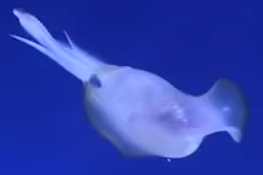
\includegraphics[height=3cm]{cuttlefish_variation1.png}}}
	\hspace{0.5cm}
	\subfloat{{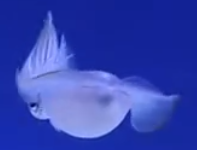
\includegraphics[height=3cm]{cuttlefish_variation2.png}}}
	\\
	\subfloat{{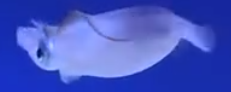
\includegraphics[height=3cm]{cuttlefish_variation3.png}}}
	\hspace{0.5cm}
	\subfloat{{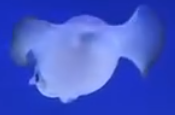
\includegraphics[height=3cm]{cuttlefish_variation4.png}}}
\caption{Différentes apparences d'une même seiches dans une vidéo.}
\label{fig:cuttlefish_variation}
\end{figure}
\FloatBarrier
\clearpage





\section{Motivation}
Le suivi d'objet, de manière générale, étant un problème que l'on rencontre dans beaucoup de domaines liés à l'informatique, les précédents exemples n'étant qu'un petit aperçu, il est donc un problème de choix à étudier lors de notre parcours d'études.\\
De plus, il permet d'introduire des concepts et des algorithmes fondamentaux, comme le concept de filtrage de signaux, ou d'espace de représentation, ou encore, les algorithmes de filtrage, de descripteurs, ou de mesures de similarité.\\
Ces concepts et algorithmes sont récurrents dans le monde de l'informatique et plus précisément quant il s'agit de faire du traitement du signal ou de la vision par ordinateur.\\
Se familiariser dès à présent avec ces différentes notions pourra grandement nous aider dans la suite de notre parcours.\\




\section{Méthodes}
Il existe beaucoup d'approches possibles pour résoudre le problème de suivi d'objet, approches parmi lesquelles ont peut noter:
\begin{itemize}
	\item \textit{Intelligence Artificielle}\newline
	Cette approche est de plus en plus populaire, notamment avec des modèles comme YOLO\cite{redmon_you_2016} ou SSD\cite{liu_ssd_2016}. Ces modèles peuvent directement donner la bounding box de l'objet suivi, sans avoir a faire de traitement sur la sortie du modèle.\\
	Cependant, cette approche est peu résistante a l'occlusion de l'objet suivi.\\
	
	\item \textit{Capteurs}\newline
	Cette approche utilise, par exemple, des IMUs ou marqueurs infrarouge, qui peuvent donner des informations sur l'accélération linéaire ou angulaire. Ces informations sont ensuite filtrées grâce à des algorithmes de filtrage, comme le filtre de Kalman (linéaire ou non), ou encore le filtre à particule.\\
	Cependant, cette approche nécessite de poser des capteurs sur l'objet à suivre.\\
	
	\item \textit{Photogrammétrie}\newline
	Cette approche utilise des descripteurs d'image pour extraire des features importantes et ensuite, matcher ces features avec d'autres images pour pouvoir estimer le déplacement de la camera.\\
	Cependant, cette approche est plus utilisée dans le cas ou l'on cherche à savoir où est-ce que le cameraman se situe, plutôt qu'un objet qui se trouve dans une image (comme le SLAM).\\
	
	\item \textit{Hybride}\newline
	Cette approche combine différentes parties des méthodes déjà présentées et est celle sur laquelle ce projet est basé.\\
	On utilise l'intelligence artificielle pour détecter un objet d'intérêt à suivre dans une séquence d'images, la partie filtrage de l'approche avec des capteurs pour améliorer nos estimations de l'état de l'objet suivi, et enfin, la photogrammétrie pour récupérer les features intéressantes dans une image et les comparer avec les features d'une image de référence.\\
	Cette approche est cependant assez sensible aux paramètres que nous lui donnons, ainsi qu'à certaines caractéristiques des images données en entrée, comme le contraste, la résolution ou encore la colorimétrie.\\
	Le détail de cette approche sera donné en partie \hyperlink{chapter.3}{3}.\\
\end{itemize}





\section{Cahier des charges}

\subsection{Besoins fonctionnels}
Les besoins peuvent être séparés en 5 catégories:
\begin{enumerate}
	\item Le besoin d'une intelligence artificielle pour effectuer la détection initiale.
	\item Le besoin de descripteurs pour récupérer un vecteur qui décrit une image donnée.
	\item Le besoin de mesures de similarité pour comparer un vecteur caractéristique d'une image avec un descripteur de référence.
	\item Le besoin d'un filtre à particule permettant d'estimer certaines propriétés de la seiche que l'on suit.
	\item Le besoin d'un programme principal permettant d'agencer chacune des parties ensemble.\\
\end{enumerate}

Les différents descripteurs et mesures de similarité devront pouvoir être utilisés par le filtre à particule afin de mettre à jour l'état de chacune des particules. Par extension, le filtre à particule devra être modulable, afin de fonctionner avec ces différents descripteurs et mesures de similarité, ainsi que de répondre aux demandes du programme principal.\\
Le programme principal se charge de l'initialisation des différents modules ainsi que de l'affichage de données clefs (visualisation de  résultats).\\

\subsection{Besoins non-fonctionnels}
Les formats vidéos acceptés sont libres.\\
La résolution des vidéos est également libre, mais une préférence sera porté pour la résolution 640x640 (résolution utilisée pour entrainer l'intelligence artificielle).\\
Le programme doit pouvoir tourner sur Windows, Linux et OSX.\\
Le programme doit pouvoir sauvegarder le résultat obtenu en une vidéo et également sauvegarder les bounding box dans un fichier texte.\\

\subsection{Contraintes}
Aucun budget n'a été alloué pour le projet, le travail s'effectuera sur nos machines personnelles, ou sur les machines mises à disposition par l'université.\\
Le projet doit être complété en 4 mois, avec une vingtaine de jours supplémentaires pour la rédaction du rapport.\\


\clearpage


\chapter{Technologies}

\clearpage

\chapter{Développements Logiciel : Conception, Modélisation, Implémentation} 

\section{Développements logiciel}
Dans le cadre du projet, plusieurs éléments ont été développé, à noter, une intelligence artificielle pour détecter des seiches dans une image, une base de donnée de seiches pour entraîner l'intelligence artificielle et un algorithme de filtre à particule utilisant des descripteurs et mesures de similarité pour calculer le poids de chaque particule.\\

\subsection{Intelligence Artificielle}
La base de donnée d'image de seiches est composée d'images provenant de vidéos de seiches prises par des plongeurs en mer, et par des particuliers dans des aquariums.\\
Chaque image a été annotée à la main par les membres du groupe en utilisant le logiciel en ligne Roboflow, la base de donnée est constituée d'un total de 5175 images.\\
L'intelligence artificielle utilise le code et les poids pré entrainé de YOLOv7\cite{wang_yolov7_nodate}, qui peuvent être trouvé sur le github officiel de YOLOv7\cite{yolov7_github}.
Cette intelligence artificielle a été entrainée pour 300 cycles de la base de donnée, soit un total de 25 heures sans interruptions.\\
Les performances obtenues sont illustrées dans la figure \ref{fig:ai_results} et des exemples sont donnés en figure \ref{fig:ai_examples}.\\

\begin{figure}[!htbp]
\center
	\subfloat[Precision]{{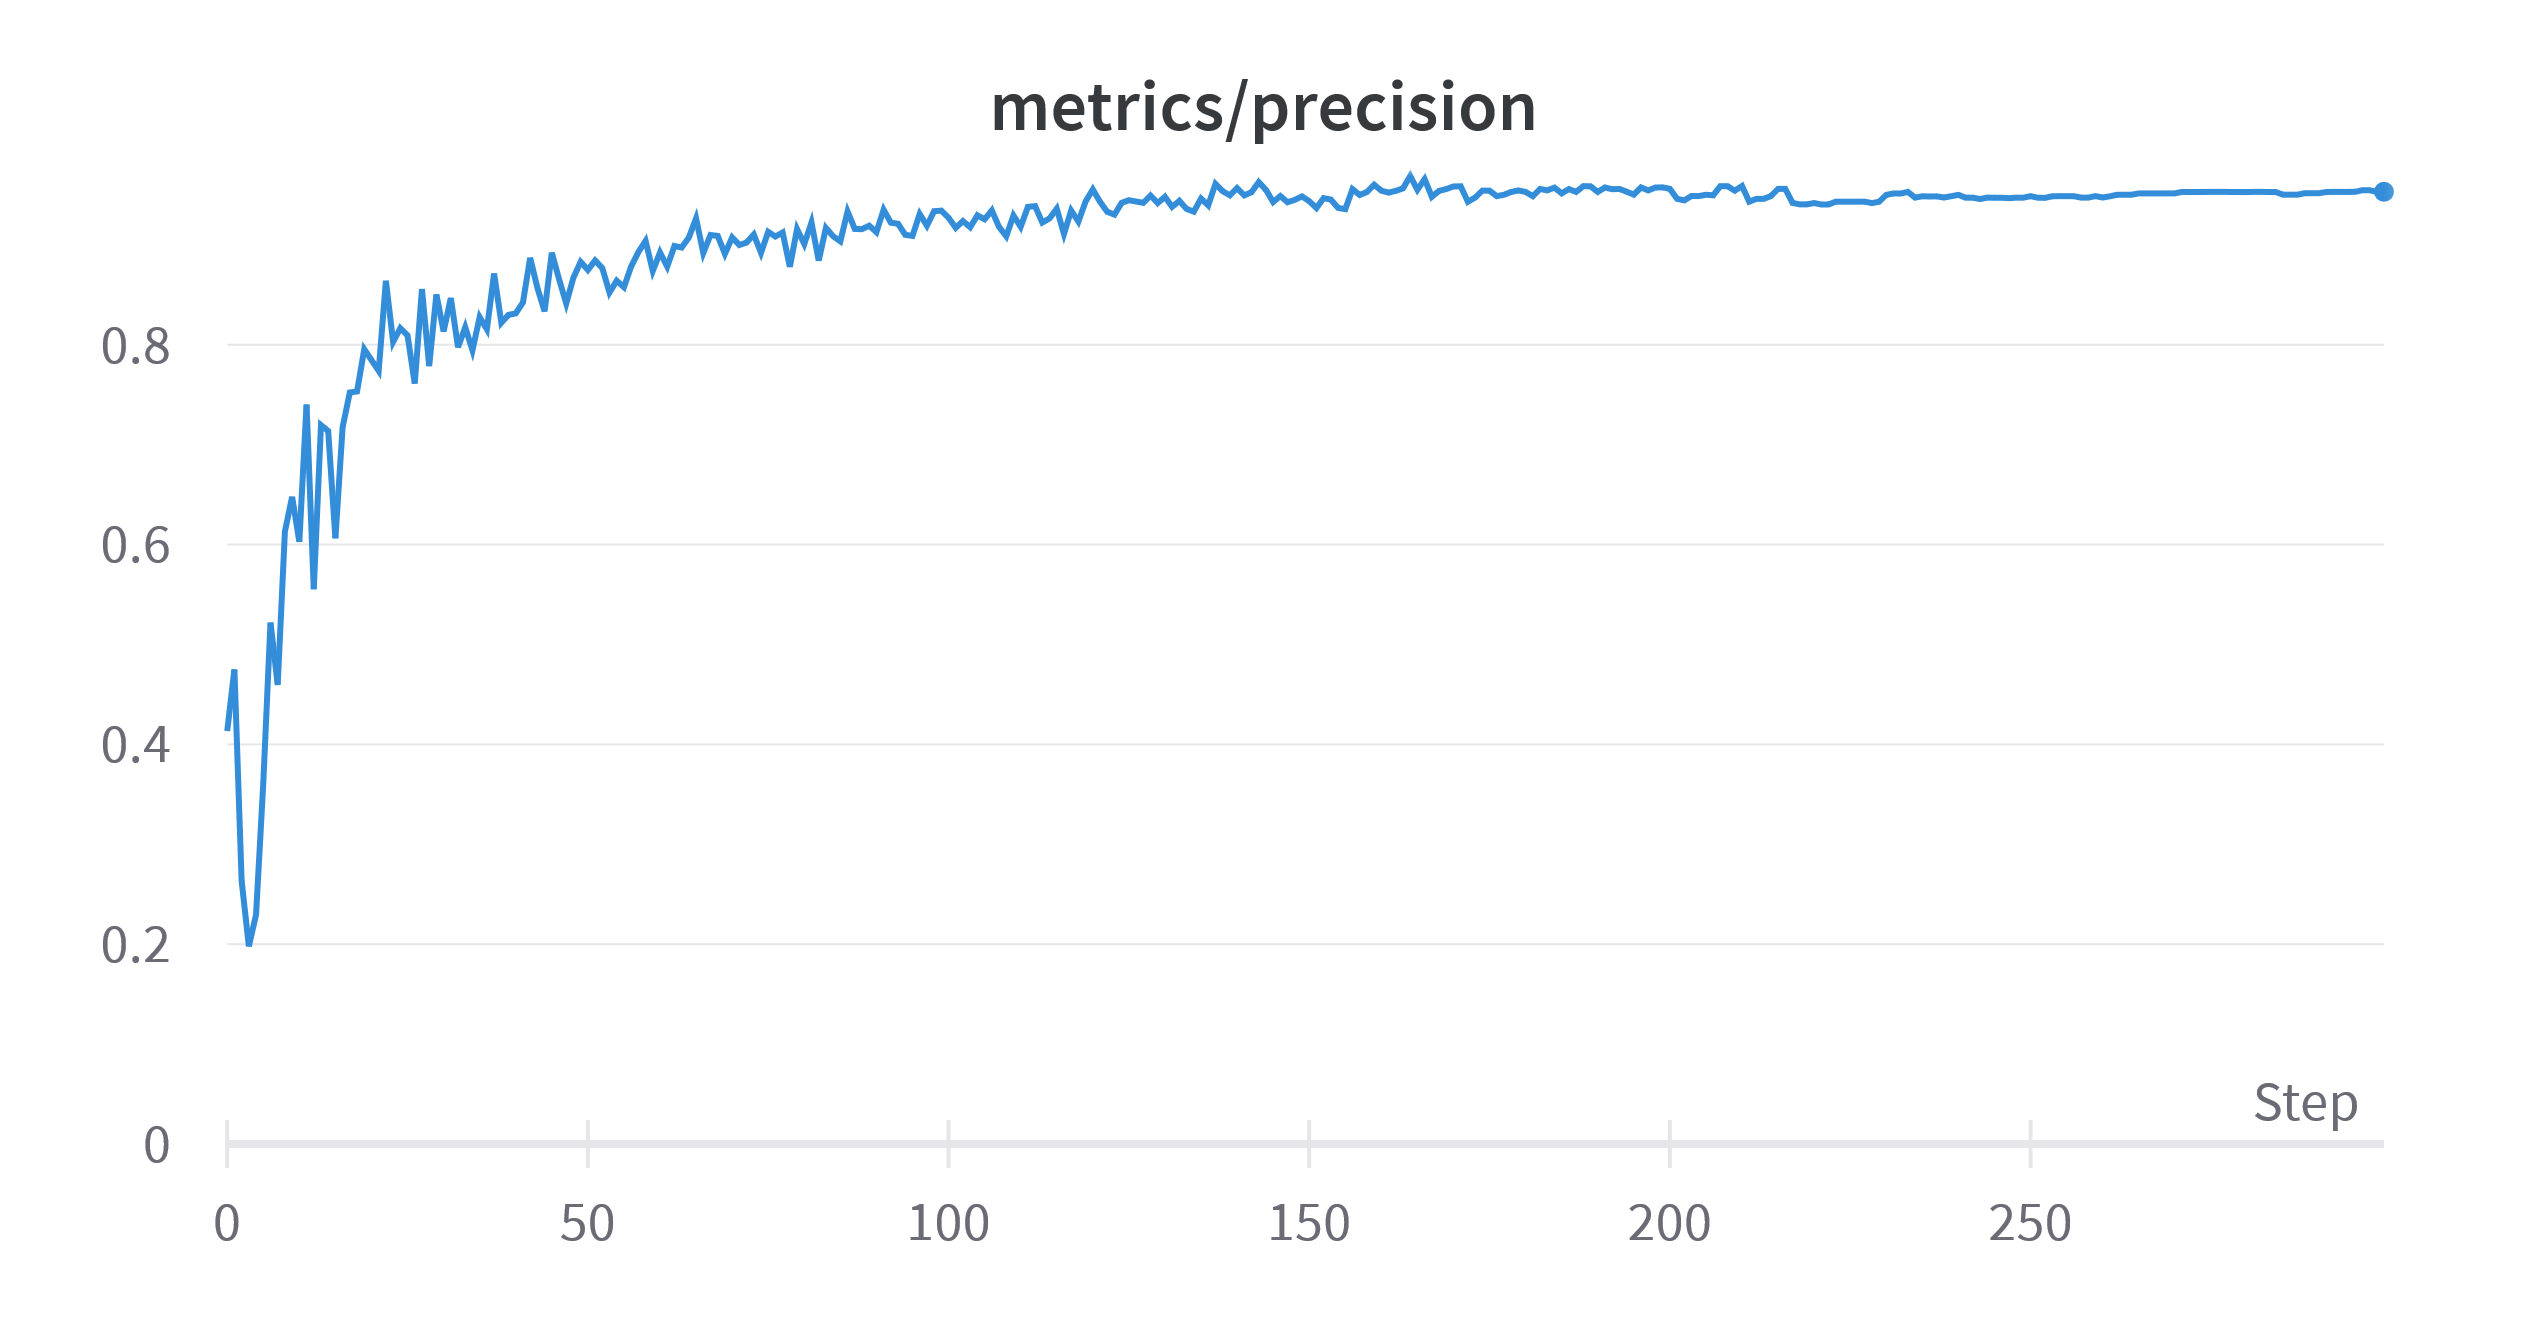
\includegraphics[scale=0.07]{metricsprecision.png}}}
	\subfloat[Recall]{{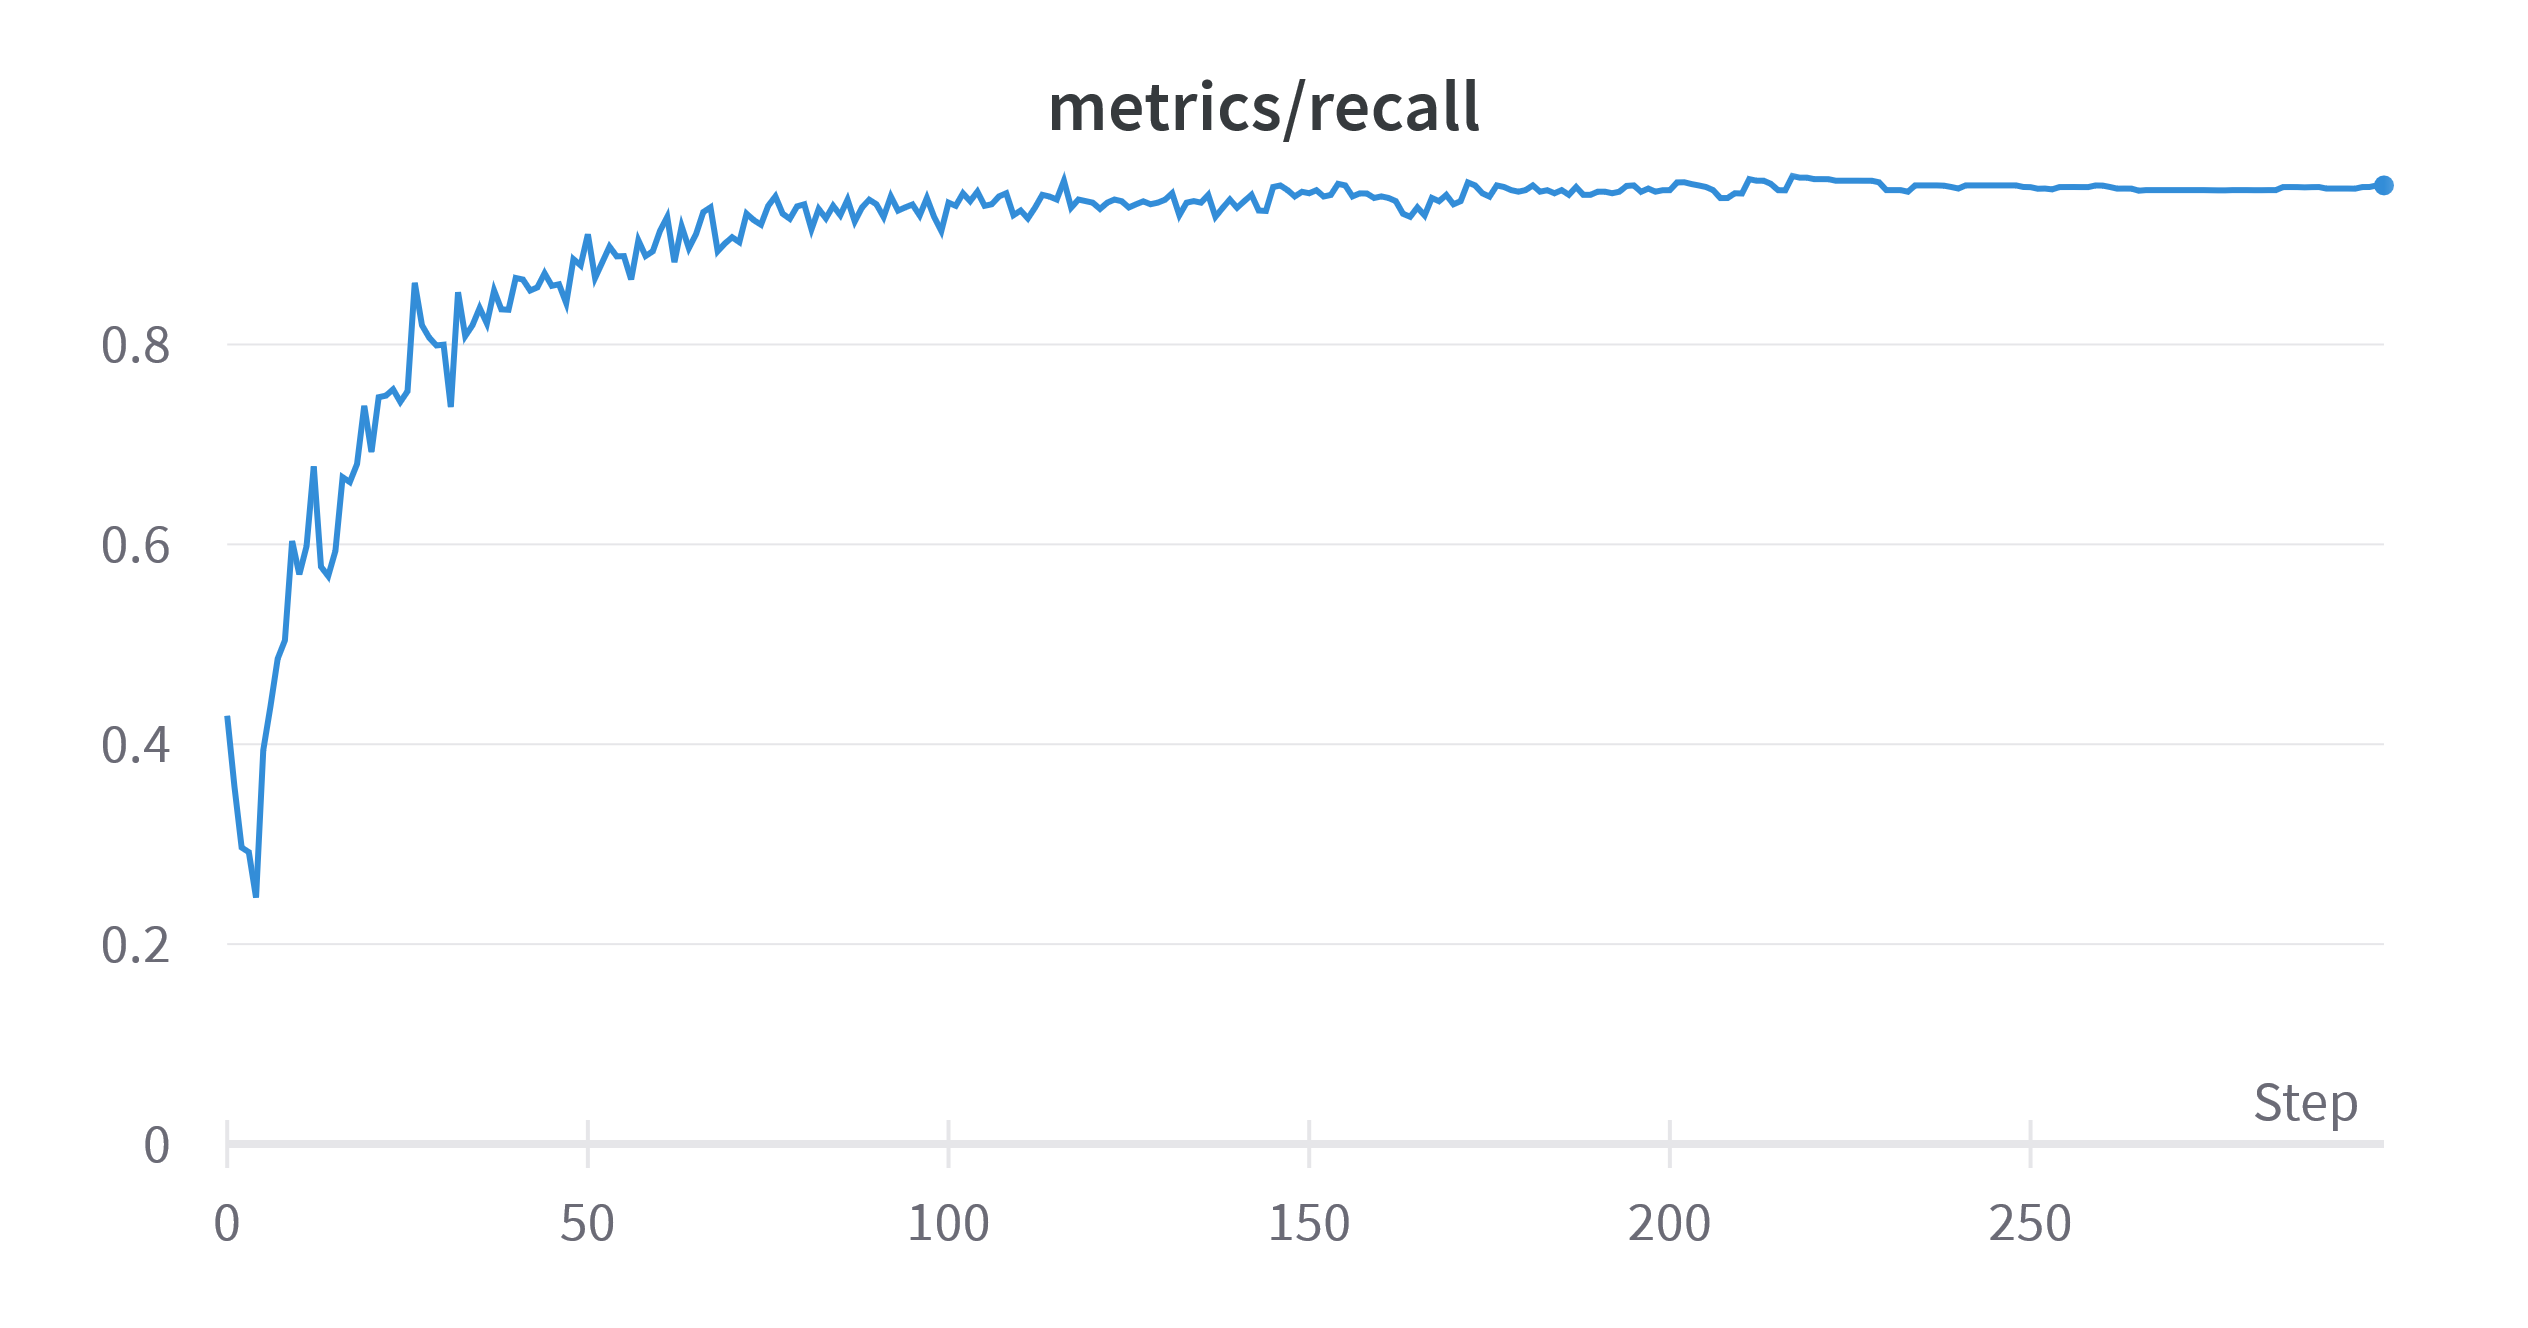
\includegraphics[scale=0.07]{metricsrecall.png}}}
	\\
	\subfloat[mAP@.5]{{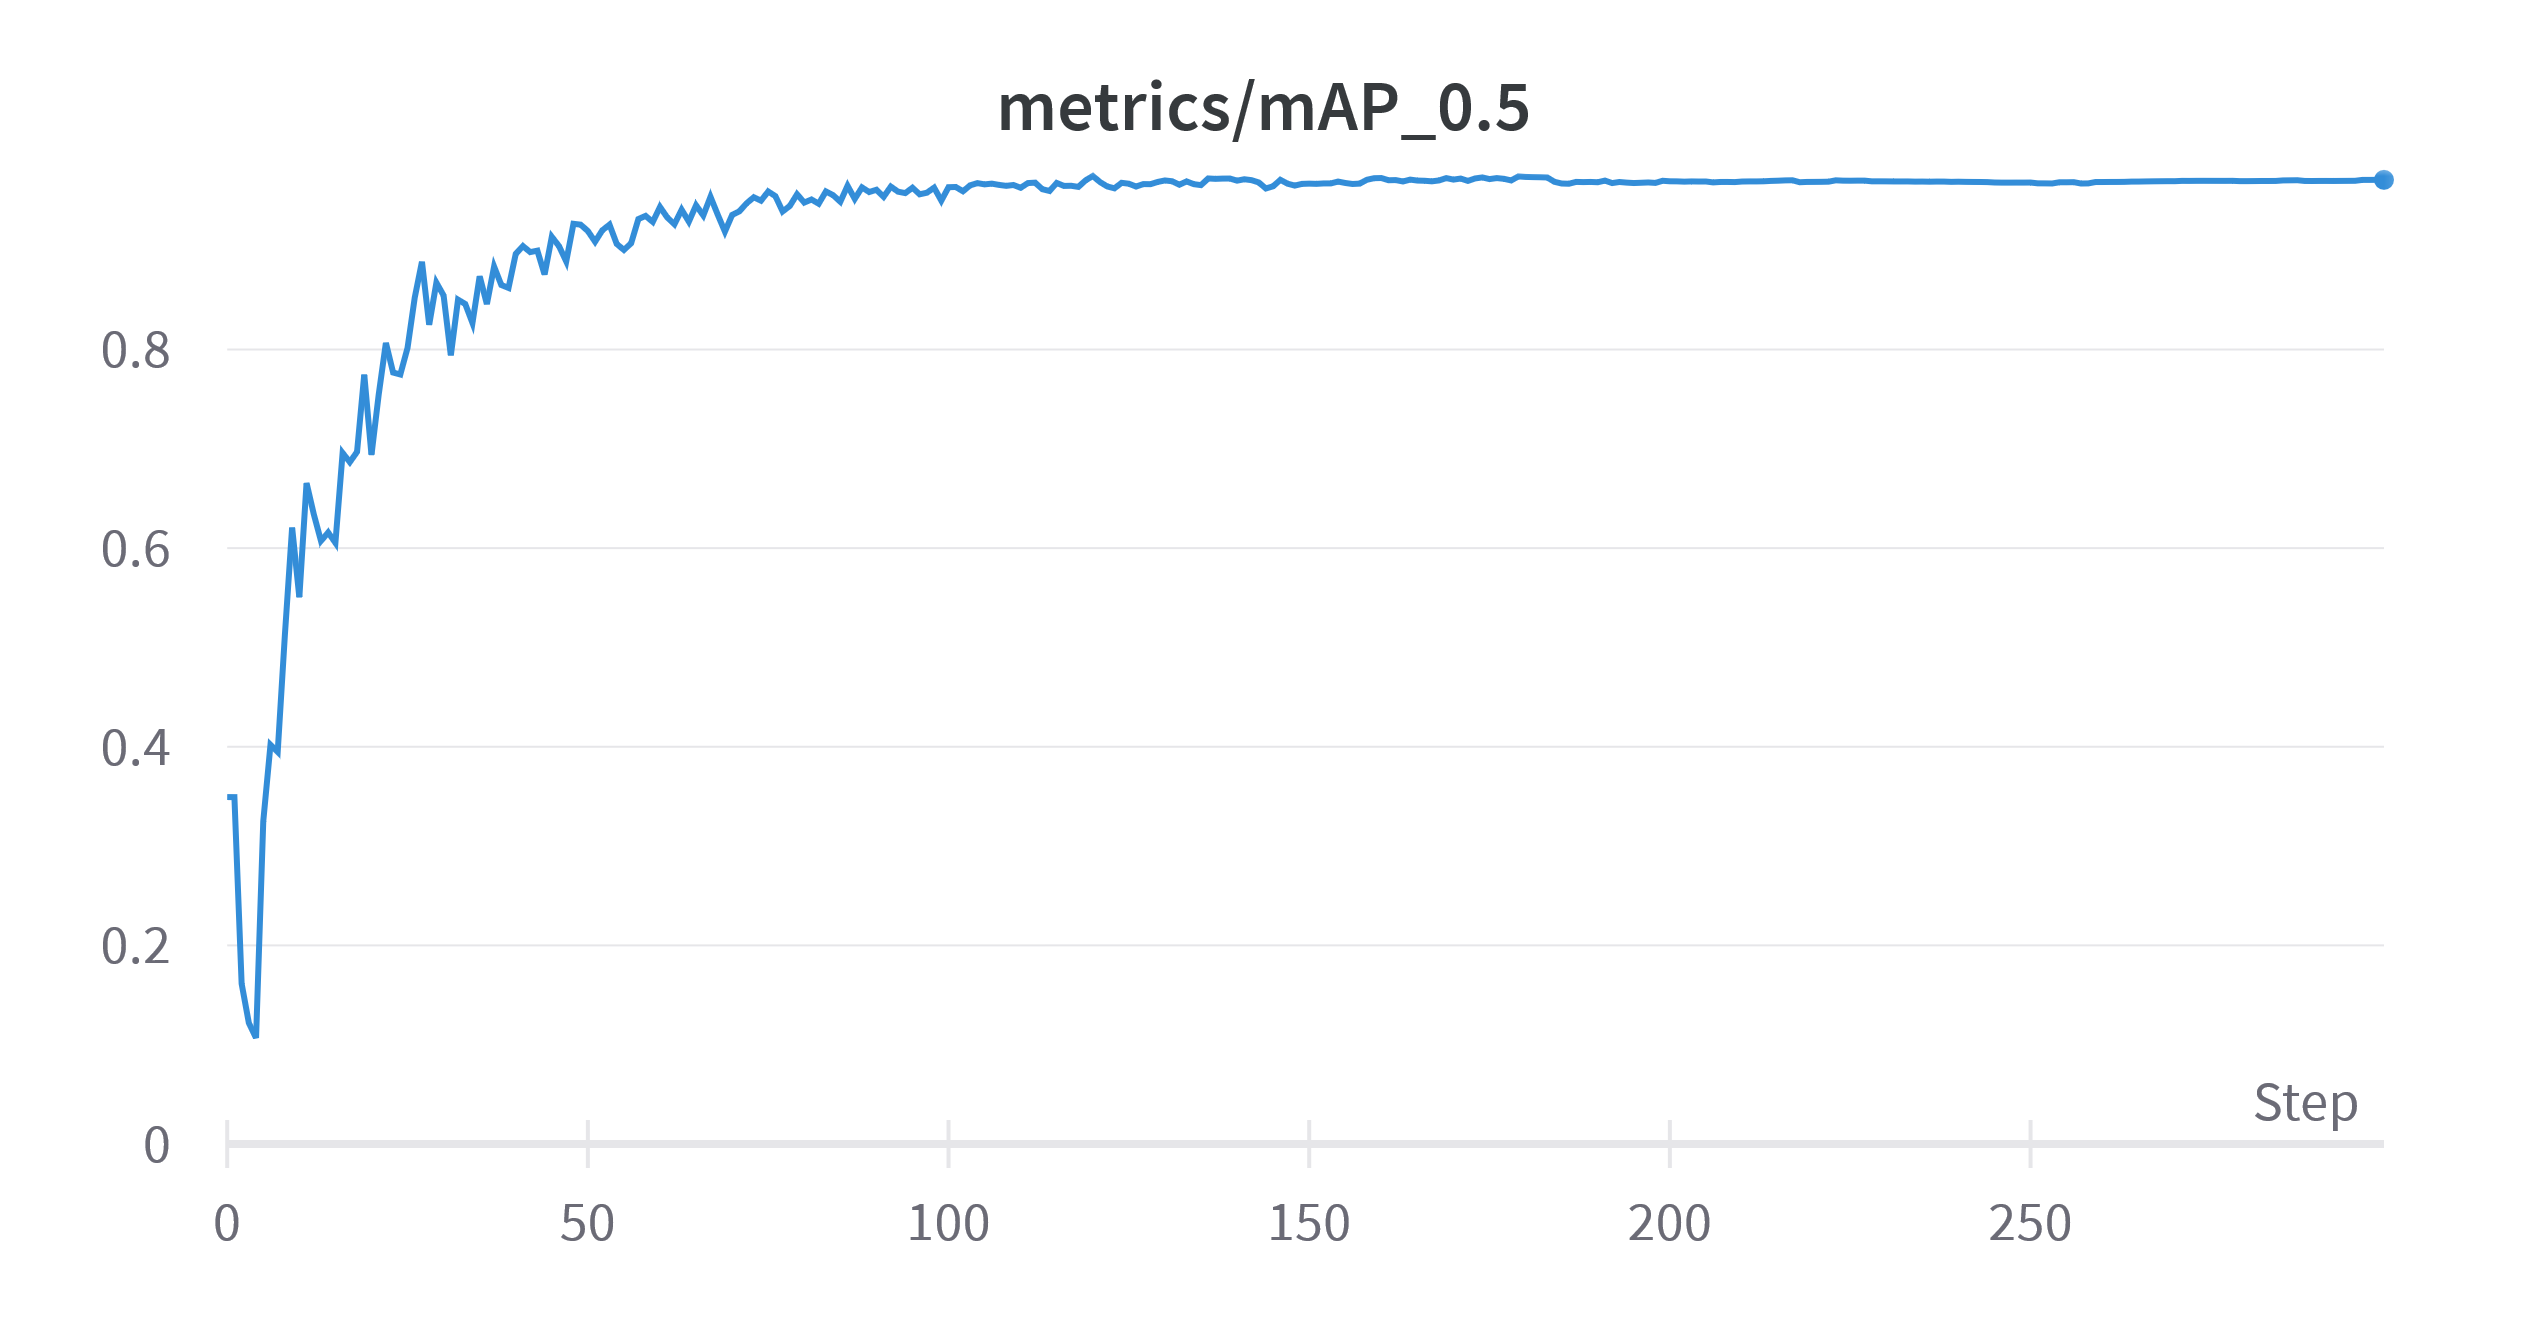
\includegraphics[scale=0.07]{metricsmAP_0.5.png}}}
	\subfloat[mAP@.5:.95]{{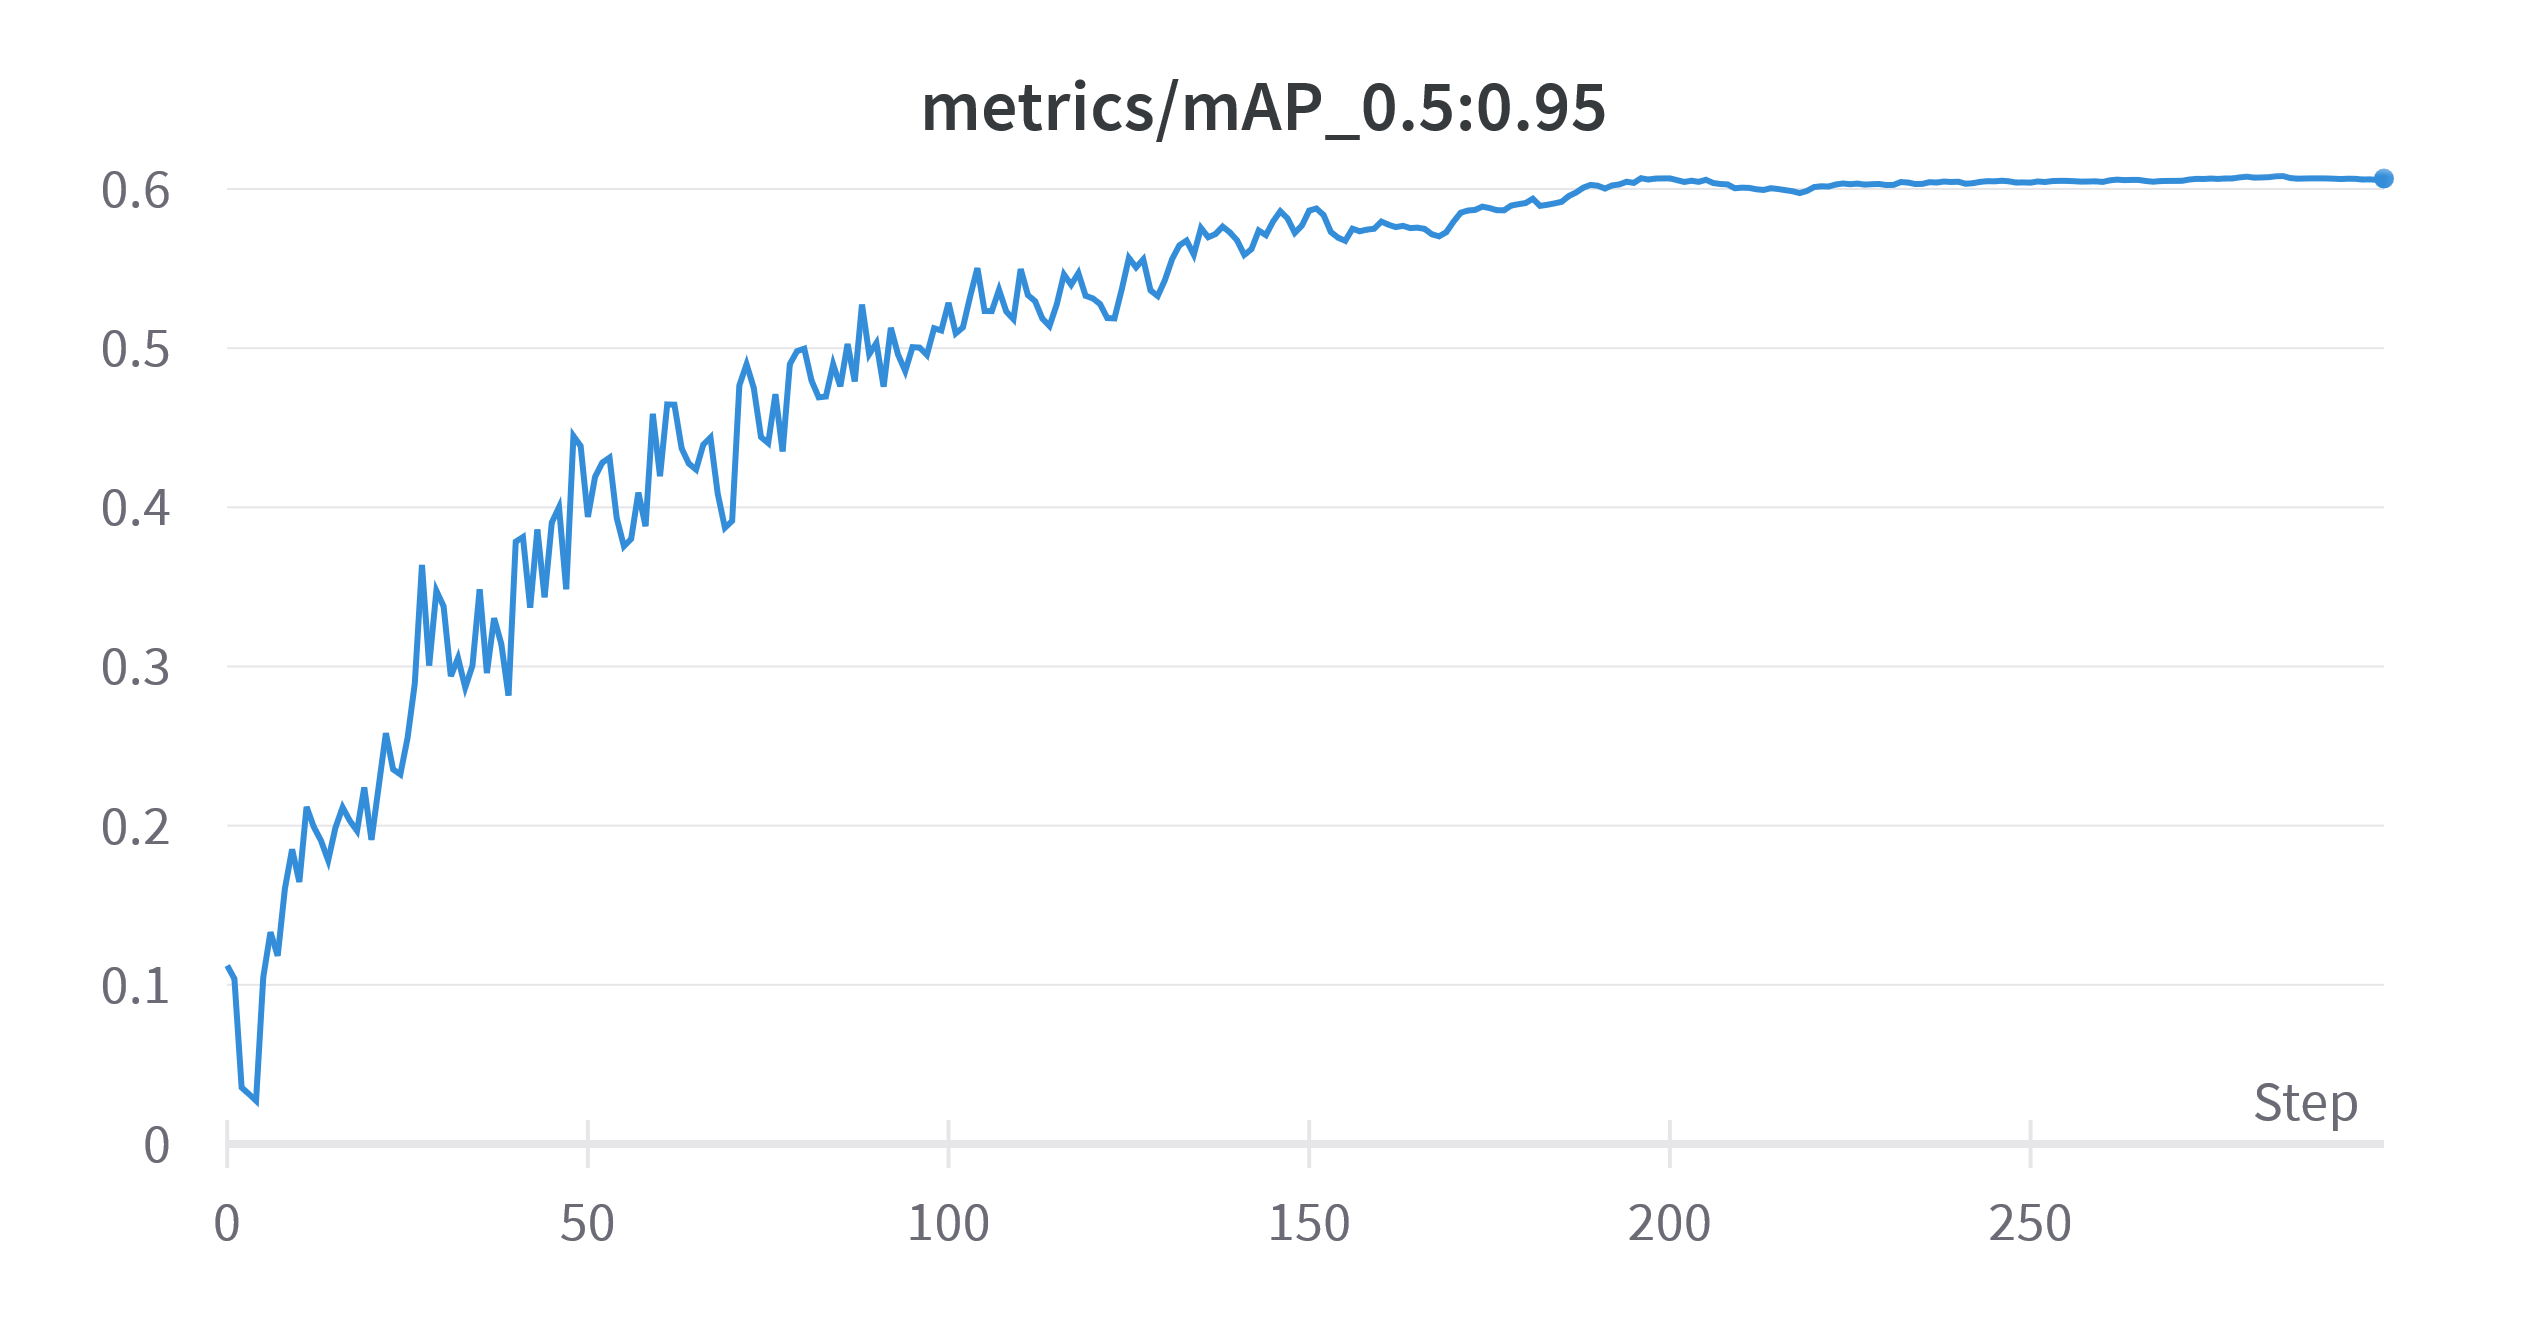
\includegraphics[scale=0.07]{metricsmAP_0.5_0.95.png}}}
\caption{Performances de notre modèle après entrainement.}
\label{fig:ai_results}
\end{figure}
\FloatBarrier

Les différentes définitions peuvent être retrouvées en annexe (\ref{app:mAP}).\\
%Nombre de vrai positif divisé par le nombre de vrai positif plus le nombre de faux positif
%Nombre de vrai positif divisé par le nombre de positif total
\\
Les résultats obtenus sont compilés dans le tableau suivant:\\
\begin{center}
\begin{tabular}{|c|c|c|c|}
	\hline
	Précision & Recall & mAP@.5 & mAP@.5:.95\\
	\hline
	0.953 & 0.959 & 0.971 & 0.607\\
	\hline
\end{tabular}
\end{center}

\begin{figure}[!htbp]
\center
	\subfloat{{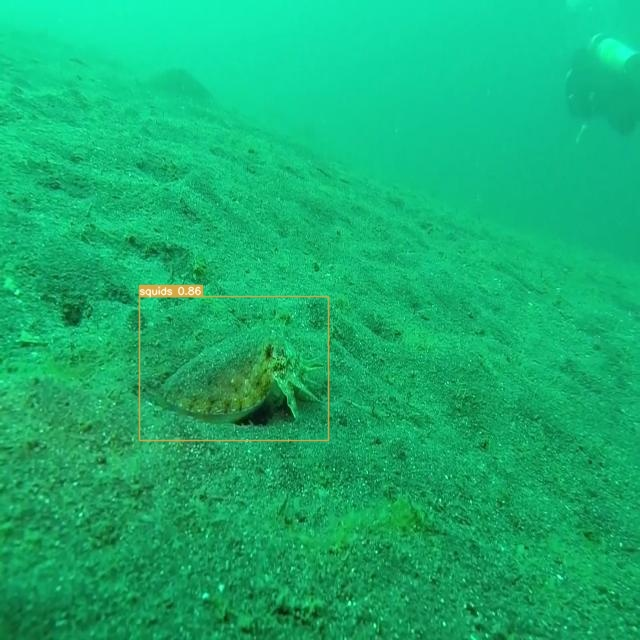
\includegraphics[scale=0.3]{cuttlefish_example1.jpg}}}
	\hspace{0.1cm}
	\subfloat{{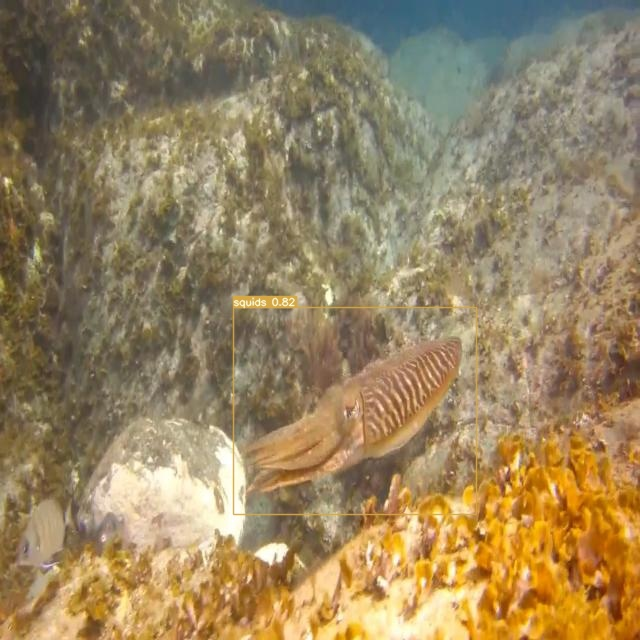
\includegraphics[scale=0.3]{cuttlefish_example2.jpg}}}
	\\
	\subfloat{{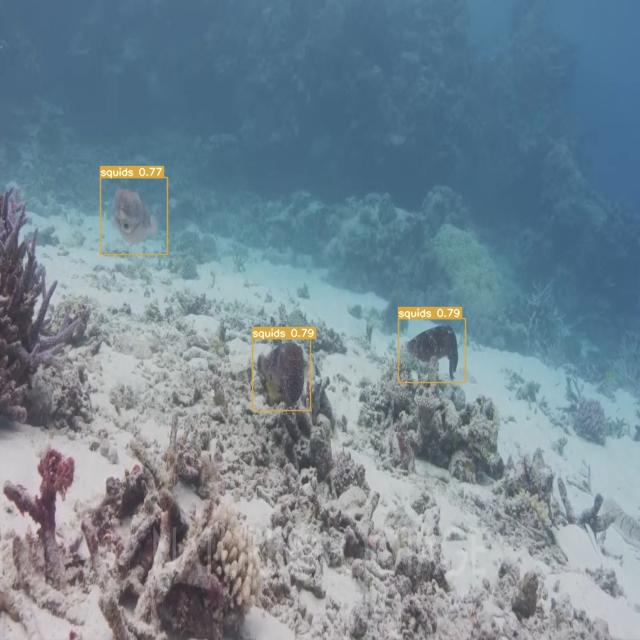
\includegraphics[scale=0.3]{cuttlefish_example3.jpg}}}
	\hspace{0.1cm}
	\subfloat{{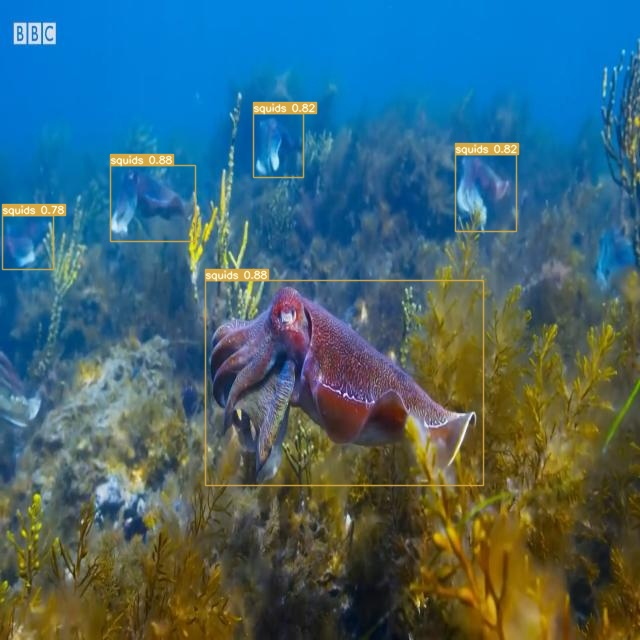
\includegraphics[scale=0.3]{cuttlefish_example4.jpg}}}
\caption{Exemples de résultats obtenus par notre modèle.}
\label{fig:ai_examples}
\end{figure}
\FloatBarrier



\subsection{Logiciel de suivi de seiche}
Ce logiciel est composé d'un filtre à particule, de descripteurs, et de mesures de similarité, qui seront développés en partie \hyperlink{chapter.4}{4}.\\
Il prend en entrée une liste de paramètres pour configurer les différentes parties, et une vidéo. Après configuration du filtre à particule, du descripteur et de la mesure de similarité, la première image de la vidéo est donnée à notre intelligence artificielle, pour avoir une estimation de la position et bounding box d'une seiche que l'on souhaite suivre dans la vidéo.\\
Après le traitement de la première image par notre intelligence artificielle, chaque image de la vidéo est donnée au filtre à particule afin qu'il mette à jour toutes ses particules, et estime au mieux la position et la bounding box de la seiche suivie.\\
Une fois que le filtre à particule a fini de traiter une image, celle-ci est affichée avec la position estimée en bleu et la bounding box estimée en vert, et les meilleures particules en rouge (voir figure \ref{fig:soft_result}). Le numéro de l'image traitée est affiché en haut à gauche de la fenêtre.\\

\begin{figure}[!htbp]
\center
	\subfloat{{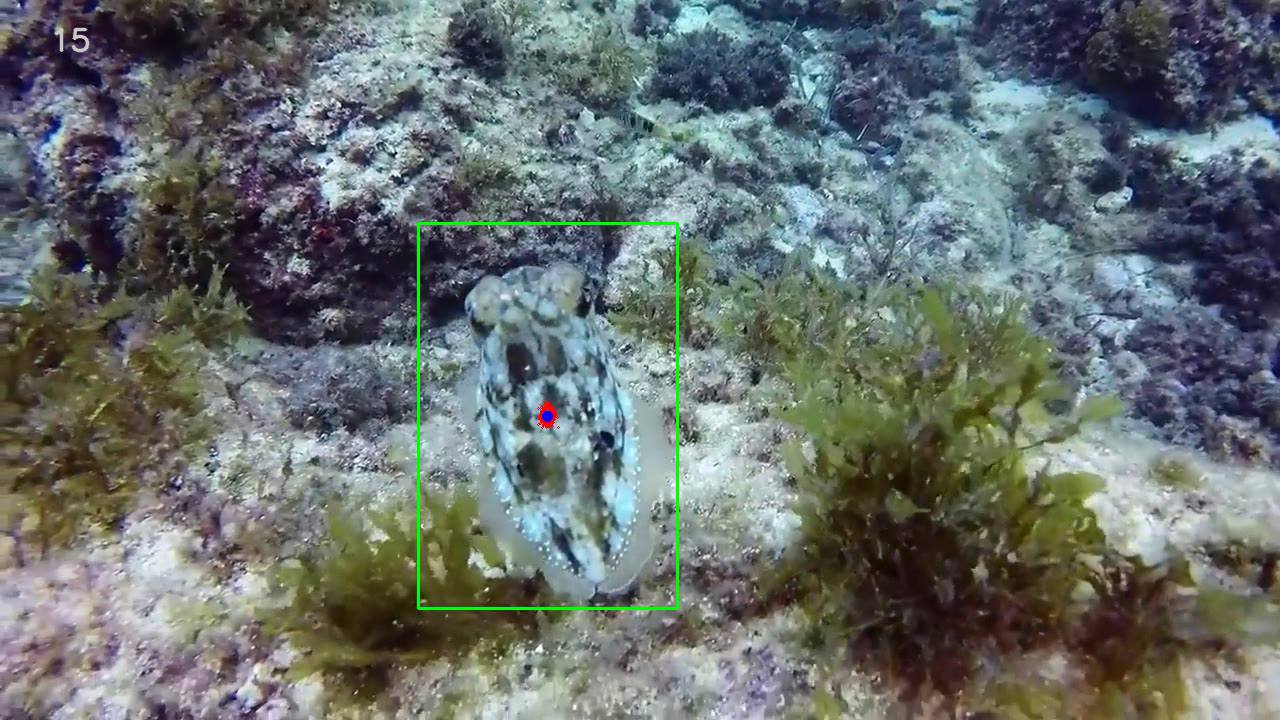
\includegraphics[scale=0.3]{Cuttlefish_results0013.png}}}
\caption{Exemple d'une image renvoyé par le logiciel.}
\label{fig:soft_result}
\end{figure}
\FloatBarrier

Le logiciel donne également la possibilité de sauvegarder la vidéo résultante, ainsi que les valeurs de la particule estimée à chaque itération du filtre.\\
Sauvegarder cette estimation permet, par la suite, d'effectuer une analyse des performances de nos solutions, en utilisant un script d'évaluation qui calcule l'IoU (voir annexe \ref{app:IoU}) entre une estimation à un instant $t$ et la véritable valeur à ce même instant, comme montré dans la figure \ref{fig:eval_result}.\\

\begin{figure}[!htbp]
\center
	\subfloat{{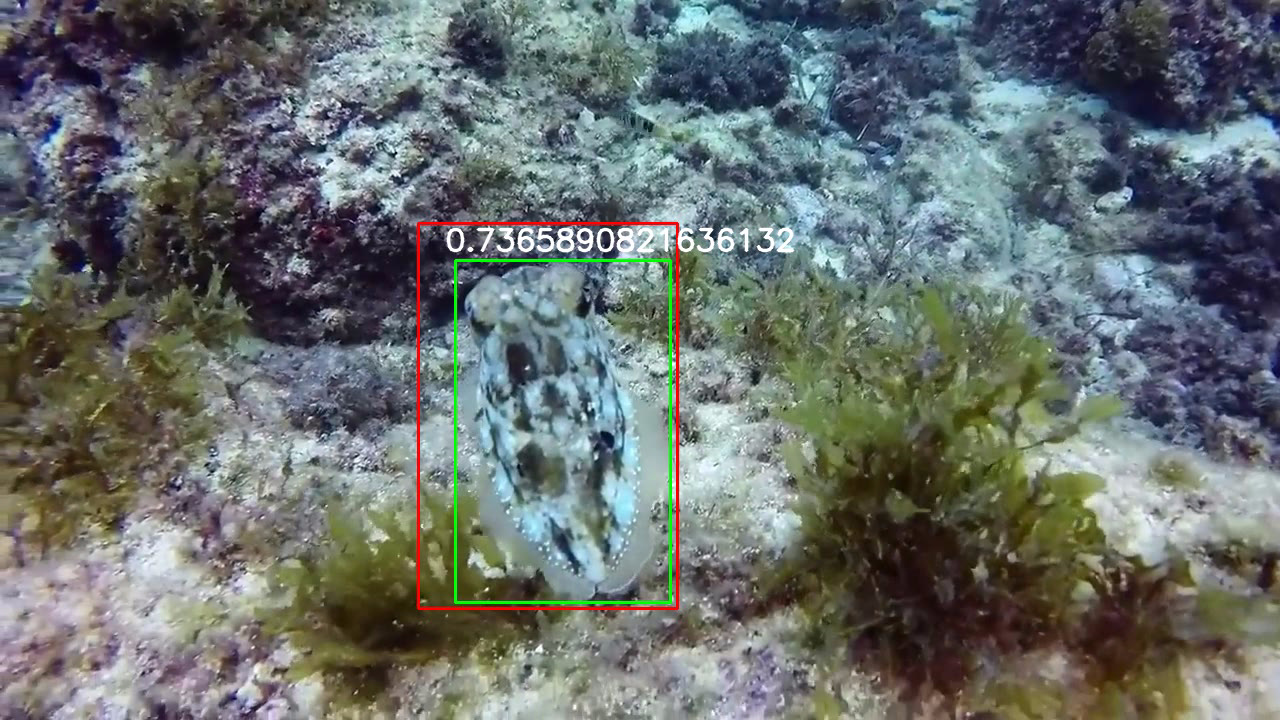
\includegraphics[scale=0.3]{eval0014.png}}}
\caption{IoU (blanc) entre l'image de référence (vert) et notre résultat (rouge).}
\label{fig:eval_result}
\end{figure}
\FloatBarrier


\clearpage
\section{Modules}
Le diagramme UML de cas d'utilisation (figure \ref{fig:uml_diagram_usecase}) du projet est assez simple, et se résume à une unique relation entre l'utilisateur et le logiciel, celle de lancer le programme avec une vidéo et les paramètres souhaités. Le reste des relations est effectué en interne et aucune interaction externe n'est requise.\\
Le diagramme UML global des classes peut être retrouvé en annexe \ref{app:UMLGlobal}.

\begin{figure}[!htbp]
\center
	\subfloat{{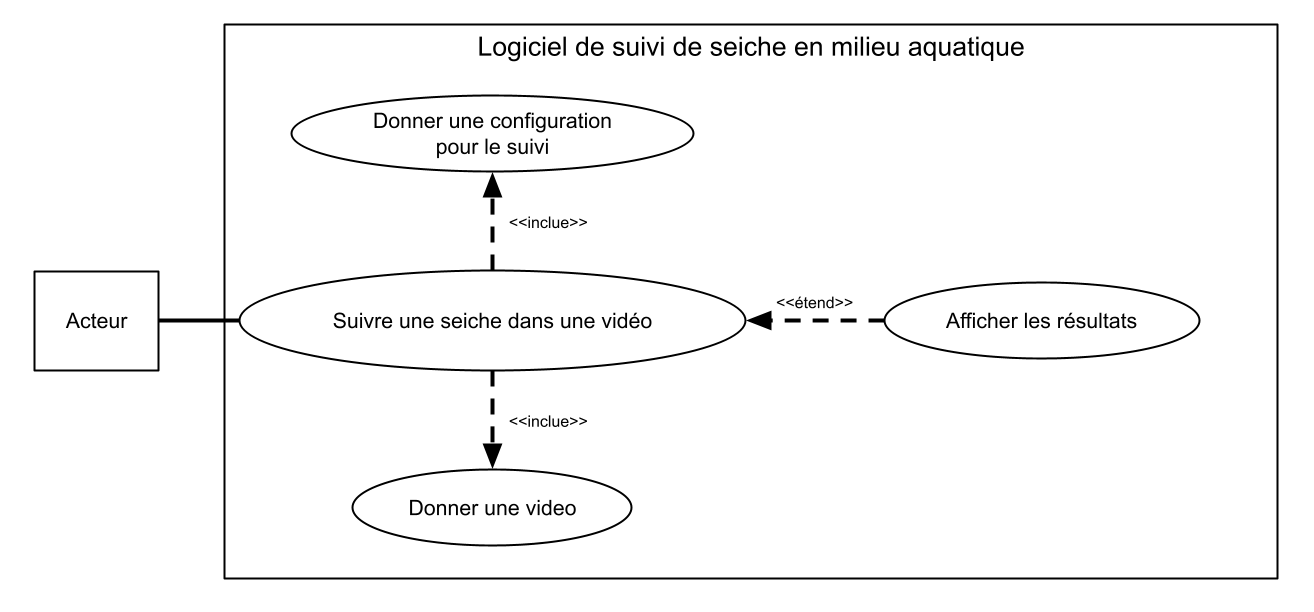
\includegraphics[scale=0.4]{usecase.png}}}
\caption{Diagramme UML de cas d'utilisation.}
\label{fig:uml_diagram_usecase}
\end{figure}
\FloatBarrier


\subsection{Descripteurs}
Le module descripteur est constitué d'une classe parent $Descriptor$ qui possède 5 classes filles, $HOG$, $HOGCASCADE$, $HOGCOLOR$, $LBP$ et $HOGCASCADELBP$. Ces classes sont les différents descripteurs que l'utilisateur peut utiliser dans le filtre à particule.\\
Toutes ces classes possèdent 2 méthodes communes, la méthode $update$ qui permet de mettre à jour certains paramètres du descripteur, et la méthode $compute$ qui permet d'effectuer le calcul du descripteur sur une liste d'images.\\
A noter, que les descripteurs $HOGCASCADE$ et $HOGCOLOR$ sont des variantes du descripteur $HOG$ (HOG et HOG cascade seront détaillés en partie \hyperlink{chapter.4}{4}), et le descripteur $HOGCASCADELBP$ est une combinaison entre un descripteur HOG cascade et LBP.\\
\\
Ce module permet de calculer, pour chaque particule du filtre, un vecteur descripteur qui pourra, par la suite, être comparé avec un descripteur de référence pour estimer la similarité entre la particule et une particule de référence.\\
Le diagramme UML du module est donné en figure \ref{fig:uml_diagram_descriptor}.

\begin{figure}[!htbp]
\center
	\subfloat{{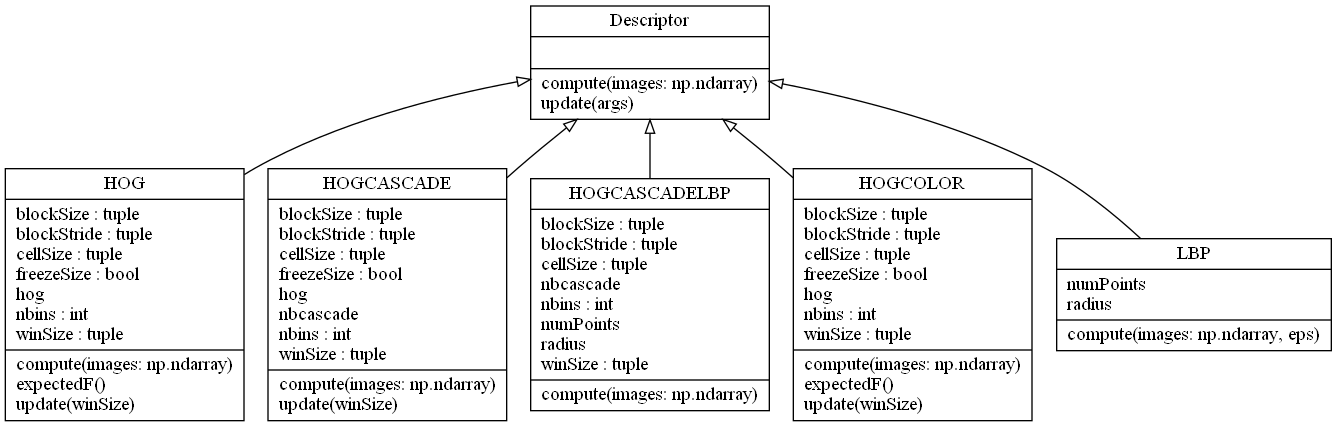
\includegraphics[scale=0.4]{descriptors.png}}}
\caption{Diagramme UML des classes du module descripteur.}
\label{fig:uml_diagram_descriptor}
\end{figure}
\FloatBarrier




\subsection{Mesure de similarité}
Le module mesure de similarité est constitué d'une classe parent $Similarity$ qui possède 4 classes filles, $Bhattacharyya\_sqrt$, $Bhattacharyya\_log$, $Cosine\_Similarity$ et $Kullback\_Leibler\_Divergence$. Ces classes sont les différentes mesures de similarité que l'utilisateur peut utiliser dans le filtre à particule.\\
Toutes ces classes possèdent une méthode commune, la méthode $computeSimilarity$ qui permet de calculer la similarité entre une liste de vecteurs descripteur et un vecteur descripteur de référence.\\
Les mesures de similarité $Bhattacharyya\_sqrt$ et $Cosine\_Similarity$ seront détaillées en partie \hyperlink{chapter.4}{4}.\\
\\
Ce module permet de calculer, pour chaque descripteur de chaque particule du filtre, un coefficient de similarité qui indique quelles particules sont les plus probables de représenter la position de la seiche à un instant $t$.\\
Le diagramme UML du module est donné en figure \ref{fig:uml_diagram_similarity}.

\begin{figure}[!htbp]
\center
	\subfloat{{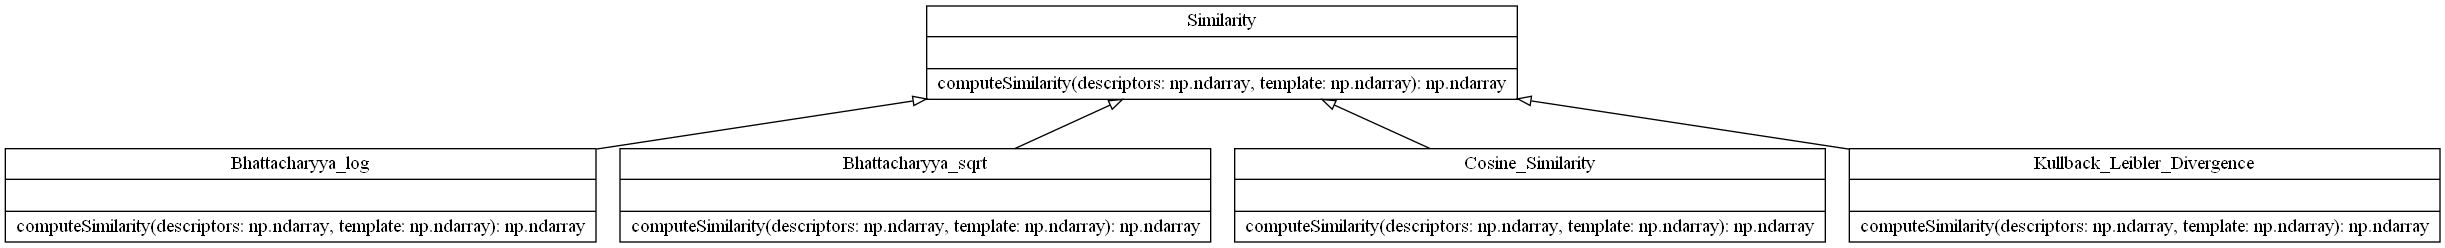
\includegraphics[scale=0.2]{similarity.png}}}
\caption{Diagramme UML des classes du module mesure de similarité.}
\label{fig:uml_diagram_similarity}
\end{figure}
\FloatBarrier




\subsection{Filtre à particule}
Le module filtre à particule est le plus conséquent, car il regroupe plusieurs autres modules, comme les modules descripteur et mesure de similarité. La classe $ParticleFilter$ est la classe principale de ce module et implémente l'algorithme du filtre à particule. Elle fait appel aux classes $Particle$, $Descriptor$, $Slicer$, $Resampling$ et $Similarity$, et les utilisent ensemble pour effectuer le suivi d'une seiche.\\
\\
Ce module est responsable de fournir tous les résultats nécessaires au programme principal, pour qu'il puisse les afficher et/ou les sauvegarder pour être finalement évalués. Ce module est très flexible et permet d'être configuré avec différentes structures de particules, différents descripteurs, différentes mesures de similarité, ou encore différentes méthodes de ré-échantillonnage.\\
Le diagramme UML du module est donné en figure \ref{fig:uml_diagram_particlefilter}.

\begin{figure}[!htbp]
\center
	\subfloat{{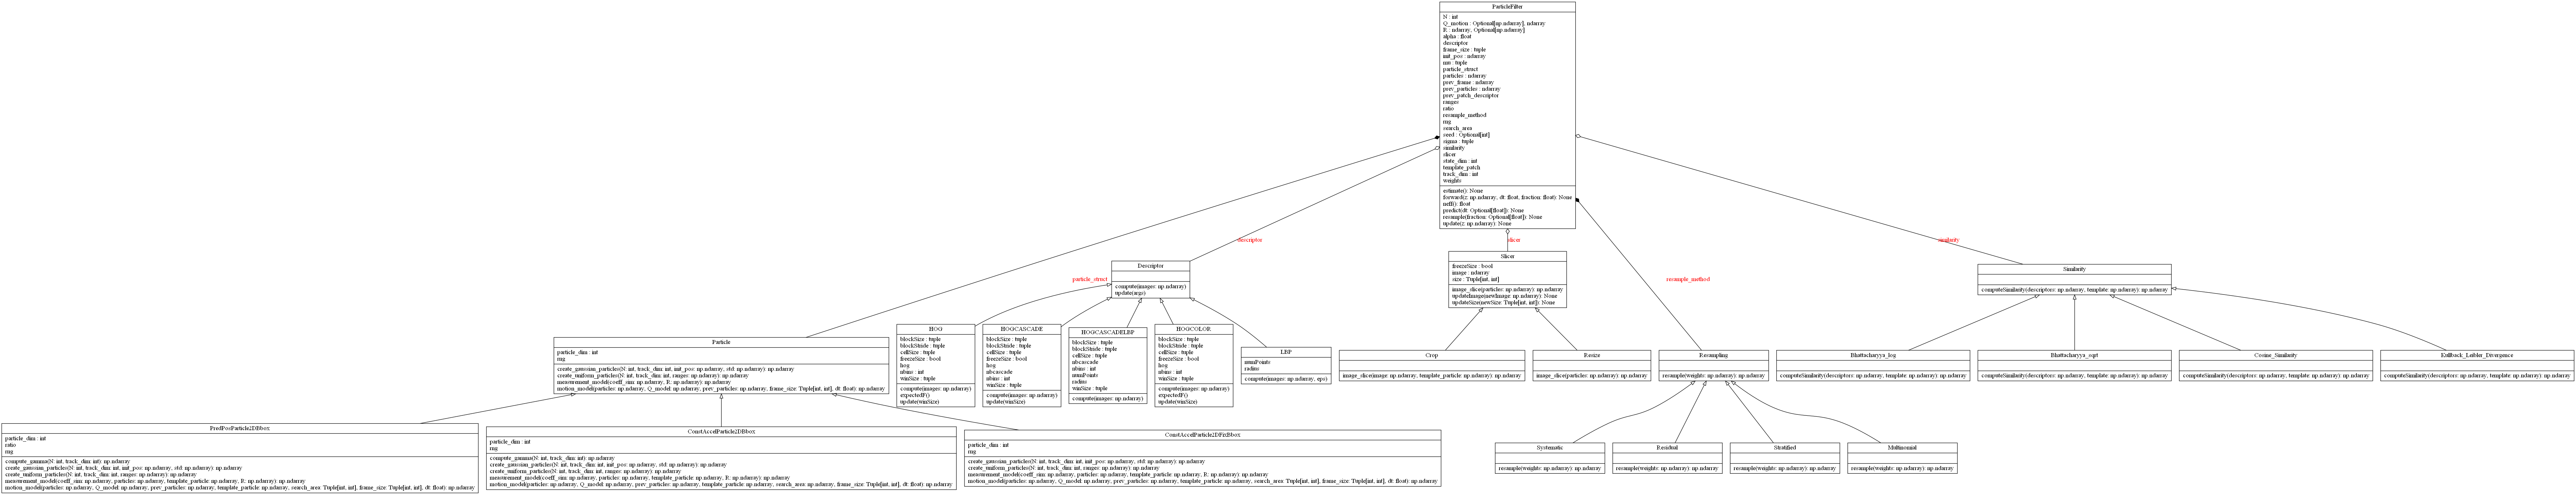
\includegraphics[scale=0.065]{particlefilter.png}}}
\caption{Diagramme UML des classes du module filtre à particule.}
\label{fig:uml_diagram_particlefilter}
\end{figure}
\FloatBarrier





\section{Structures de données}
Les structures de données principales du projet sont les tenseurs en tant que tableaux multidimensionnels, pour ce faire, nous utilisons la librairie Numpy, qui permet de réaliser des opérations sur ces tableaux de façon optimisée.\\
Nous essayons de garder les données un maximum sous ce format, pour éviter les conversions et opérations qui pourraient ralentir le logiciel de suivi. C'est pour cela que la majorité des entrées des programmes réalisés demande des 'ndarray', qui est le type des tableaux Numpy.\\
\\
Les images prises en entrée des programmes sont transformées en tableau Numpy, selon la convention de OpenCV, c'est-à-dire avec les couleurs au format BGR et la hauteur de l'image comme première dimension du tenseur, et la largeur de l'image comme seconde dimension.\\
\\
L'utilisateur du logiciel n'intervient qu'à un seul niveau dans le programme, le reste des entrées du logiciel est géré en interne afin de préserver au mieux l'intégrité des données traitées.\\
L'utilisateur peut uniquement donner des paramètres au logiciel lorsqu'il le lance, ces paramètres sont alors parsés en différent arguments qui sont vérifiés par le programme, puis utilisés pour initialiser les différents modules, afin de commencer le suivi d'une seiche.




\section{Statistiques}
Le projet compte un total de 25 classes réparties dans 10 scripts python (voir figure \ref{fig:uml_diagram_classes}).\\
Les scripts et classes de YOLOv7\cite{wang_yolov7_nodate} utilisés dans le projet ne sont pas comptés.\\
Le projet compte en tout 1587 lignes de code.\\
L'entièreté du projet est en accès libre sur github (\cite{pp2pf}).

\clearpage


\chapter{Algorithmes et Analyse}




\section{Descripteurs}
Pour pouvoir appliquer notre mesure de similarité entre deux images et calculer les poids de nos particules, on a besoin de pouvoir extraire de l'information de nos images. Ainsi allons nous utiliser des descripteurs. \\
Un descripteur est un morceau d'information extrait d'une image sous forme de vecteur. Il permettra de reconnaitre un motif ou une structure spécifique au cours de notre vidéo. Pour calculer un descripteur on s'appuie sur l'information bas niveau de nos images (valeur des pixels, contours, gradients, ...).

\subsection{Histogramme de gradient orienté}

Nous utiliserons en particulier les histogrammes de gradients orientés (HOG) qui sont des descripteurs proposés par Navneet DALAL et Bill TRIGGS \cite{dalal_histograms_2005}. Ils correspondent à la distribution de l'orientation des contours locaux d'une image. \\

Les HOG sont calculés par DALAL et TRIGGS ainsi : \\

Une première étape de pré-traitement de l'image afin de normaliser les couleurs et d'appliquer une correction gamma à celle-ci puis la convertir en niveau de gris. Ici la normalisation du HOG est suffisante et cette étape est donc facultative, on s'est contenté de la conversion en niveau de gris. \\

L'étape suivante est le calcul de la carte des gradients en x et en y qui correspondent respectivement à la variation horizontale et verticale des gradients. On effectue une convolution centrée sur le pixel cible. Parmi les différents filtres possibles, les masques que nous utilisons sont $[-1, 0, 1]$ pour les gradients en x et $[-1, 0, 1]^{T}$ pour les gradients en y, aussi appelés filtres de Sobel. Ces masques se sont révélés plus performants dans la littérature \cite{dalal_histograms_2005}.\\

À partir de ces deux cartes de gradients on pourrait calculer la carte des modules des gradients. Néanmoins, afin d'augmenter l'efficacité du descripteur, le HOG n'est pas directement calculé à partir de l'image.\\

En effet l'image est divisée en "cellules", elles-mêmes regroupées en "blocs". On choisit des cellules de 6*6 pixels et des blocs de 3*3 cellules.\\

Pour chaque bloc, on calcule le HOG de chaque cellule. Le HOG du bloc correspond à la concaténation du HOG des cellules le composant. Pour une meilleure invariance face à l'illumination et à l'ombrage on effectue une normalisation du HOG du bloc (norme euclidiennne). Pour un vecteur x, on a :

\[ \sum_{k=0}^{n} (x_{k})^{2} \]

Donc le HOG de l'image est la concaténation de l'ensemble des HOG de chacun de ses blocs.

\begin{figure}[!htbp]
\center
	\subfloat{{
\includegraphics[height=3cm]{Squid_colors_2resized.png}}}
\caption{Bloc d'un HOG.}
\label{fig:cuttlefish_bloccells}
\end{figure}

Les histogrammes sont construits grâce aux mesures des angles des gradients et à leurs intensités. De la même manière qu'avec la taille des blocs et des cellules, on doit choisir la structure de notre histogramme. Étant donné que nous travaillons sur des angles, nous choisirons un histogramme à neuf classes et nous utiliserons des angles non signés (compris entre $[0; 180°]$).
Ainsi pour un pixel $p(x,y)$ l'angle est défini par :

\[ angle_{p} = |\arctan (\grad y, \grad x)*\frac{180}{\pi}| \]

De même que son intensité par :

\[ intensite_{p} = \sqrt{\grad x^{2} + \grad y^{2}} \]

Pour chaque pixel, on répartit son intensité proportionnellement dans les deux classes les plus proches de l'angle qui lui est associé. 
Par exemple, prenons $\grad x = 10$ et $\grad y = 10$ on obtient une intensité d'environ $14.14$ et un angle de $45°$. De cette manière la classe centrée en $40$ recevra les trois quarts ($1 - |\frac{5}{20}|$)et la classe centrée en $60$ recevra le quart restant($1 - |\frac{15}{20}|$) de l'intensité.\\

% Note : prendre gradx = grady = sqrt(2) est plus stylé mais je sais pas si c'est sage

Enfin pour affiner notre descripteur nous effectuerons le déplacement du bloc suivant :

\[ \frac{T_{cellule} * T_{bloc}}{2} \]

$T_{cellule}$ est la taille en pixels de la cellule,
$T_{bloc}$ est la taille en nombre de cellules d'un côté du bloc.
Ainsi on a : $\frac{6*3}{2} = 9$, de plus, un bloc faisant plus de 9 pixels de côté, on a un chevauchement des blocs et donc des pixels pris en compte plusieurs fois. Cela permet au vecteur de mieux caractériser l'image cible.

\begin{figure}[!htbp]
\center
	\subfloat{{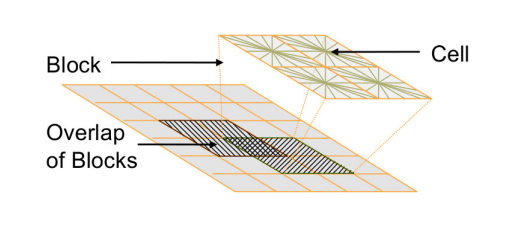
\includegraphics[height=3cm]{blocoverlap.png}}}
\caption{Déplacement d'un bloc.}
\label{fig:blocOverlap}
\end{figure}

\subsection{HOG en cascade}

Pour enrichir notre vecteur caractéristique on peut utiliser HOG en cascade qui combine les HOG de l'image à différentes résolutions. Pour procéder on calcule les HOG sur une succession de sous-régions inclusives et les ajoutons au HOG global, comme décrit dans l'article \cite{qiang_zhu_fast_2006}. De cette manière on ajoute de l'information spatiale à notre descripteur.

\begin{figure}[!htbp]
\center
	\subfloat{{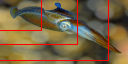
\includegraphics[height=3cm]{Squid_colors_2hogc.png}}}
\caption{HOG en cascade.}
\label{fig:cuttlefish_hog}
\end{figure}




\section{Mesures de similarité}
Après avoir obtenu les vecteurs descripteurs de chaque particule, nous les comparons avec le vecteur descripteur de référence.\\
Pour comparer deux vecteurs descripteur, nous utilisons des mesures de similarité, qui nous indiquerons si les deux vecteurs sont plus ou moins similaire. La mesure de similarité donne 0 si les vecteurs sont exactement similaire, et 1 si ils sont complètement opposés.

\subsection{Distance de Bhattacharyya}
La distance de Bhattacharyya, comme définit dans l'article \cite{bhattacharyya_measure_1960}, permet de calculer une distance entre deux lois de probabilité discrètes. Elle est définie pour deux lois $X$ et $Y$ par la formule:
$$D_{B}(X, Y) = \sqrt{1 - BC(X, Y)}$$
ou bien encore, par la formule:
$$D_{B}(X, Y) = -\ln(BC(X, Y))$$

Où $BC(X, Y)$ est appelé coefficient de Bhattacharyya et est définit par la formule:
$$\sum_{k \in X \hspace{0.1cm} ou \hspace{0.1cm} k \in Y} \sqrt{X(k)*Y(k)}$$


\subsection{Cosine similarity}
La similarité cosinus (Cosine similarity), est une distance, un score, basé sur le cosinus de l'angle entre deux vecteurs.\\
Donc, à partir d'un vecteur descripteur X et du vecteur descripteur de référence Y, nous pouvons calculer le cosinus de l'angle formé par les deux vecteurs, qui est donné par la formule:
$$Sc(X, Y) = \frac{X \cdot Y}{\|X\|\|Y\|}$$\\


\clearpage
\section{Filtre à particule}
Le filtre à particule, aussi connu sous le nom de bootstrap, ou algorithme de condensation, est basé sur une méthode de Monte Carlo, c'est à dire utiliser un ensemble de particule discrète pour représenter la densité de probabilité associé au système que l'on souhaite modéliser. L'idée principale du filtre à particule est d'approcher une distribution, impossible ou difficile à estimer directement, grâce à un ensemble d'échantillons pondérés $S=\{(X_{n}, w_{n})|n=1...N\}$, où $X_{n}$ indique la nième particule, $w_{n}$ indique l'importance de la particule, ou le poids de celle-ci, et $N$ est le nombre total de particule. Plus d'information peuvent être trouvé aux références suivantes \cite{russell_norvig} et \cite{rlabbe}.\\
\\
Cet algorithme a, par exemple, pu être utilisé avec le descripteur HOG, comme dans ces articles \cite{xu_human_2010}, \cite{kong_particle_2019}, \cite{qiang_zhu_fast_2006} et \cite{dalal_histograms_2005}, mais il peut également être utilisé avec d'autre descripteur, ou combinaison de descripteur, comme HOG cascade combiné avec LBP (Local Binary Pattern).\\
\\
Les particules que le filtre utilise peuvent être définies de plusieurs façon, nous avons choisi de définir une particule, comme un point en 2D, la vélocité et l'accélération de ce point, et la demi largeur et demi hauteur de la bounding box délimitant notre cible, mais il est possible de changer cette définition. A un instant $t$, une particule est donc représentée par un vecteur à 8 dimensions:
$$X^{t}=\left[ x^{t}, \dot{x}^{t}, \ddot{x}^{t}, y^{t}, \dot{y}^{t}, \ddot{y}^{t}, l^{t}, h^{t} \right]^{T}$$
Où $(x^{t}, y^{t})^{T}$, $(\dot{x}^{t}, \dot{y}^{t})^{T}$ et $(\ddot{x}^{t}, \ddot{y}^{t})^{T}$ sont les coordonnées, vélocités et accélération du centre de notre cible en pixel, respectivement, $(l^{t}, h^{t})$ décrit la bounding box de notre cible en pixel avec la demi largeur et la demi hauteur.\\
\\
Bien qu'il existe plusieurs variantes de cet algorithme, le principe général reste le même (voir figure \ref{alg:particlefilter_basic}). Il s'agit d'utiliser les particules pour déterminer l'état de notre système à un instant $t$, en faisant une prédiction de nos particules dans le temps puis en ajoutant du bruit, et en combinant cette prédiction avec une observation $z$ (résultats de capteurs, ou images d'une vidéo, par exemple) afin de mettre à jour les poids de chacune des particules. Une fois les poids mis à jour, on vérifie combien de particule participent réellement à l'estimation de l'état de notre système, et si ce nombre est en dessous d'un certain seuil, on effectue une étape de ré-échantillonnage en gardant les particules de poids fort, et en supprimant celles de poids faible. Finalement, on peut estimer l'état de notre système, en prenant la moyenne pondérée de nos particules (MLE, Maximum Likelihood Estimation) ou en prenant comme estimation la particule de poids le plus fort (MAP, Maximum A Posteriori).

\begin{algorithm}
	\caption{Filtre à particule général}\label{alg:particlefilter_basic}
	\KwData{Une observation $z$}
	\KwResult{Une estimation de l'état de notre système}
	\ForEach{Particules p}{
		Prédiction de $p$ grâce à un modèle de prédiction $f$ et $\nu$ du bruit blanc: $\hat{X}_{p}^{t} = f(X_{p}^{t-1}, \nu)$\\
		Traitement de l'observation grâce à un modèle de mesure $h$ et $n$ le bruit de l'observation: $z^{t} = h(z, n)$\\
		Combinaison de $\hat{X}_{p}^{t}$ avec $z^{t}$ pour mettre à jour le poids de $p$: $w_{p}^{t}$
	}
	Normalisation des poids des particules: $$w_{p}^{t} = \frac{w_{p}^{t}}{\sum_{i=0}^{NB_{particule}} w_{i}^{t}}$$
	\If{le nombre de particule effective est inférieur à un certain seuil}{
		Ré-échantillonnage des particules pondérées par leur poids
	}
	Estimation de l'état de notre système:
	$$(MLE) \hspace{0.4cm} X^{t} = \frac{1}{NB_{particule}} * \sum_{p=0}^{NB_{particule}} X_{p}^{t}*w_{p}^{t}$$
	ou
	$$(MAP) \hspace{0.4cm} X^{t} = \underset{p}{\arg\max} \hspace{0.2cm} w_{p}^{t}$$
\end{algorithm}

Dans notre cas, le modèle de mesure sera effectué en calculant la similarité entre un descripteur de référence $F_{ref}$ et les descripteurs de chaque particule. Au préalable, chaque particule ce voit associer un patch de l'image courante qui est récupéré en utilisant la position et la bounding box de la particule, puis en dimensionnant le patch obtenu à une dimension fixée en amont par l'utilisateur.\\
Cette liste de patch est ensuite donnée à une fonction de mesure de similarité, qui, pour chacun des patch, renvoi un coefficient de similarité ($coeff\_sim$).\\
Ces coefficients de similarité sont ensuite utilisés pour calculer le poids de chaque particule, grâce à une distribution gaussienne centrée en 0 et de déviation standard $\sigma$ (dans notre cas $\sigma=n$, le bruit de l'observation):
$$w_{p}^{t} = \frac{1}{\sqrt{2\pi\sigma^{2}}}e^{-\frac{(coeff\_sim_{p})^{2}}{2\sigma^{2}}}$$
Après estimation de l'état de notre système, nous calculons le descripteur associé à cet état et remplaçons le descripteur de référence $F_{ref}$ par celui-ci.\\
\\
Le modèle de prédiction, quant à lui, utilise la méthode des différences finies d'ordre 3, c'est-à-dire que nous considérons les trois derniers états de la particule pour calculer sa position, vélocité et accélération actuelle. Cependant, d'autres modèle auraient pu être choisi, comme le modèle de prédiction utilisant les équations physique du mouvement, qui a aussi été implémenté.\\
La méthode des différences finies est basée sur les formules suivante:
\begin{equation} \label{eq:vel}
\begin{split}
\dot{x}^{t} = \frac{x^{t} - x^{t-1}}{dt}\\
\dot{y}^{t} = \frac{y^{t} - y^{t-1}}{dt}
\end{split}
\end{equation}
\vspace{0.4cm}
\begin{equation} \label{eq:accel}
\begin{split}
\ddot{x}^{t} = \frac{\dot{x}^{t} - \frac{x^{t-1} - x^{t-2}}{dt}}{dt}\\
\ddot{y}^{t} = \frac{\dot{y}^{t} - \frac{y^{t-1} - y^{t-2}}{dt}}{dt}
\end{split}
\end{equation}
\vspace{0.4cm}
\begin{equation} \label{eq:pos}
\begin{split}
x^{t+dt} = \frac{1}{2} \cdot \ddot{x}^{t} \cdot dt^{2} + \dot{x}^{t} \cdot dt + x^{t} + \nu\\
y^{t+dt} = \frac{1}{2} \cdot \ddot{y}^{t} \cdot dt^{2} + \dot{y}^{t} \cdot dt + y^{t} + \nu
\end{split}
\end{equation}

Avec $dt$ l'intervalle de temps entre chaque image de la vidéo, et $\nu$ le bruit gaussien pour la prédiction.\\
\\
Au cours de la vidéo, il arrive que la cible ce rapproche ou s'éloigne de la caméra, si les dimensions de la bounding box sont fixes, on peut perdre en qualité sur le suivi car la bounding box peut inclure trop d'éléments parasites, ou au contraire, n'inclure qu'une petite partie de la cible.\\
Pour palier ce problème, nous effectuons également une prédiction sur les dimensions de la bounding box, définit par les formules suivante, comme définit dans \cite{kong_particle_2019}:
\begin{equation} \label{eq:gamma}
\gamma=
\begin{cases}
\begin{aligned}
	-0.05,& \hspace{0.4cm}		0 \leq p \leq 0.2\\
    -0.0125,& \hspace{0.4cm}	0.2 \le p \leq 0.4\\
    0,& \hspace{0.4cm}			0.4 \le p \leq 0.6\\
    0.0125,& \hspace{0.4cm}		0.6 \le p \leq 0.8\\
    0.05,& \hspace{0.4cm}		0.8 \le p \leq 1
\end{aligned}
\end{cases}
\end{equation}
Où $p$ est un réel aléatoire entre [0,1].\\
On a alors:
\begin{equation} \label{eq:Bbox}
\begin{split}
l^{t} = l^{t-1} * (1+\gamma) + \nu\\
h^{t} = h^{t-1} * (1+\gamma) + \nu
\end{split}
\end{equation}

En assemblant chacune des parties précédentes, on obtient alors l'algorithme final du filtre à particule, dont un example avec une configuration spécifique est donné dans l'algorithme \ref{alg:particlefilter}.


\begin{algorithm}
	\caption{Filtre à particule}\label{alg:particlefilter}
	\KwData{Une vidéo sous-marine de seiche}
	\KwResult{La liste des positions et bounding box de la cible dans la vidéo}
	\ForEach{Images $t$ de la vidéo}{
		\eIf{Première image}{
			Détection de la seiche dans l'image grâce a YOLOv7\\
			Calcul du descripteur de référence : $F_{ref}^{0}$
		}{
			\ForEach{Particules p}{
				Prédiction de la position (équation \ref{eq:pos}) et de la bounding box (équation \ref{eq:Bbox}) de $p$ dans $t$ en fonction de ses états précédents\\
				Calcul du descripteur du patch correspondant à $p$: $F_{p}^{t}$\\
				Calcul du coefficient de similarité entre $F_{p}^{t}$ et $F_{ref}^{t-1}$: $coeff\_sim_{p}^{t}$\\ 
				Calcul du poids de $p$ dans $t$ :
					$$w_{p}^{t} = \frac{1}{\sqrt{2\pi\sigma^{2}}}e^{-\frac{(coeff\_sim_{p}^{t})^{2}}{2\sigma^{2}}}$$
			}
			Ré-échantillonnage des particules pondérées par leurs poids\\
			Estimation de la position et bounding box de la seiche dans $t$:
				$$X^{t}=\frac{1}{NB_{particule}}*\sum_{p=0}^{NB_{particule}} X_{p}^{t}*w_{p}^{t}$$
		}
		Mise à jour du descripteur de référence: $F_{ref}^{t}$
	}
\end{algorithm}


\clearpage


\begin{algorithm}
	\caption{Filtre à particule}\label{alg:particlefilter}
	\KwData{Une vidéo sous-marine de seiche}
	\KwResult{La liste des positions et bounding box de la cible dans la vidéo}
	\ForEach{Images $t$ de la vidéo}{
		\eIf{Première image}{
			Détection de la seiche dans l'image grâce a YOLOv7\\
			Calcul du descripteur de reference : $F_{ref}^{0}$
		}{
			\ForEach{Particules p}{
				Prédiction de la position et de la bounding box de $p$ dans $t$ en fonction de ses états précédents.\\
				Calcul du descripteur du patch correspondant à $p$ : $F_{p}^{t}$\\
				Calcul du poids de $p$ dans $t$ :
					$$w_{p}^{t} = D_{B}(F_{p}^{t},F_{ref}^{t-1})$$
			}
			Ré-échantillonnage des particules pondérées par leurs poids\\
			Estimation de la position et bounding box de la seiche dans $t$ :
				$$X^{t}=\frac{1}{NB_{particule}}*\sum_{p=0}^{NB_{particule}} x_{p}^{t}*w_{p}^{t}$$
		}
		Mise à jour du modèle de référence
	}
\end{algorithm}

\chapter{Analyse des résultats}

\section{Métrique d'évaluation IoU}
En général, Intersection over Union (IoU) (ou indice de Jaccard) est considéré comme la métrique la plus populaire pour l'évaluation de détection d'objet. Dans le domaine de la détection d'objet, IoU est utilisé pour mesurer la similarité entre la bounding box prédit $B_{p}$ et la bounding box de la vérité terrain $B_{gt}$, en mesurant l'intersection (l'aire du chevauchement) pour $B_{p}$ et $B_{gt}$, divisé par l'aire de leur union, qui est:
$$IoU=J(B_{p}, B_{gt})=\frac{aire(B_{p} \cap B_{gt})}{aire(B_{p} \cup B_{gt})}$$
 
Comme illustré en figure \ref{fig:iou_example}:

\begin{figure}[!htbp]
\center
	\subfloat{{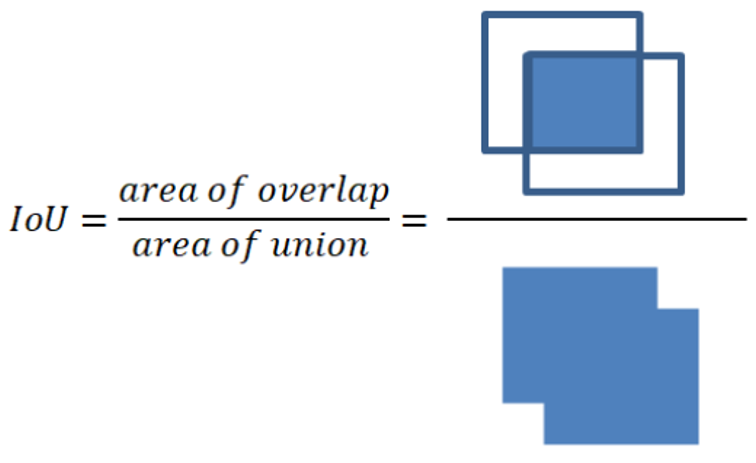
\includegraphics[scale=0.5]{IoU.png}}}
\caption{Intersection over Union (IoU)}
\label{fig:iou_example}
\end{figure}
\FloatBarrier

Dans notre cas, les bounding boxes de prédiction correspondent à la sortie de notre logiciel, ou à celle du réseau de neurone (YOLOv7). Les bounding boxes de la vérité terrain, quand à elles, correspondent à des bounding boxes annotées manuellement et qui englobe l'objet ciblé à détecter (i.e. la seiche).\\
Pour avoir la vérité terrain, nous avons utilisé LabelImg.\\
\\
Afin de classifier le résultat de la détection comme étant correcte ou non, nous comparons l'IoU à un seuil donné $T$, donc, si $IoU > T$ alors nous pouvons considérer la détection comme étant correcte, autrement, la détection est considérée comme incorrecte.\\
Dans nos testes, nous avons fixé le seuil $T$ à 0.5.



\clearpage
\section{Analyse et comparaison}
Les valeurs IoU sont calculées pour une séquence et deux approches (filtre à particule et YOLOv7), elles sont représenté dans la table \ref{tab:results}.\\
Notre méthode avec filtre à particule a réussi à détecter la seiche dans 288 des 292 frames, équivalent à 98\% du nombre total de frames, voir figure \ref{fig:pf_results}. L'IoU varie de 0.44 à 0.87 et l'IoU moyen est de 0.74.\\
YOLOv7 a réussi à détecter la seiche dans 292 des 292 frames, équivalent à 100\% du nombre total de frames, voir figure \ref{fig:yolo_results}. L'IoU varie de 0.60 à 0.90 et l'IoU moyen est de 0.76.

\begin{table}[!htbp]
\begin{tabular}{|c|c|c|c|c|c|}
\hline
Méthode & Frames & Fréquence de détection & IoU min & IoU max & IoU mean\\
\hline
Filtre à particule & 292 & 288 (98\%) & 0.44 & 0.87 & 0.74\\
\hline
YOLOv7 & 292 & 292 (100\%) & 0.60 & 0.90 & 0.76\\
\hline
\end{tabular}
\caption{Résultats pour une même séquence en utilisant notre filtre à particule et YOLOv7.}
\label{tab:results}
\end{table}
\FloatBarrier

\begin{figure}[!htbp]
\center
	\subfloat[Frame 25]{{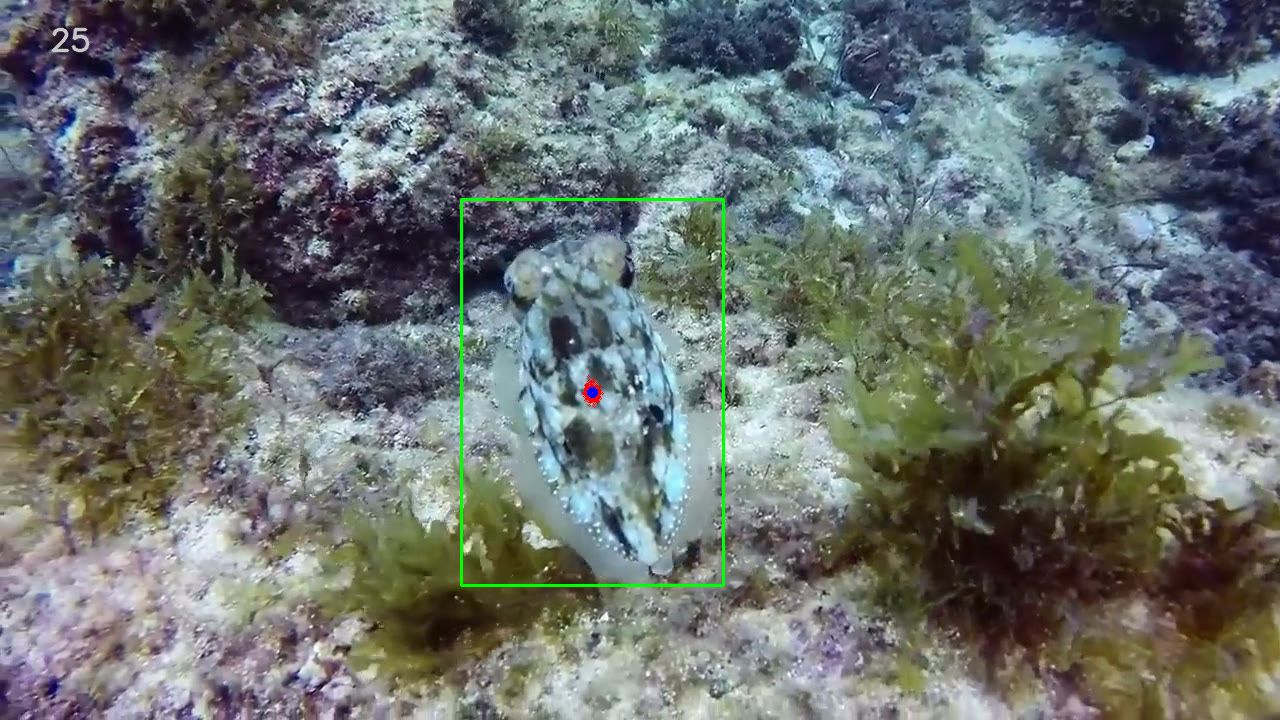
\includegraphics[scale=0.15]{result_pf_valid_1.png}}}
	\hspace{0.1cm}
	\subfloat[Frame 50]{{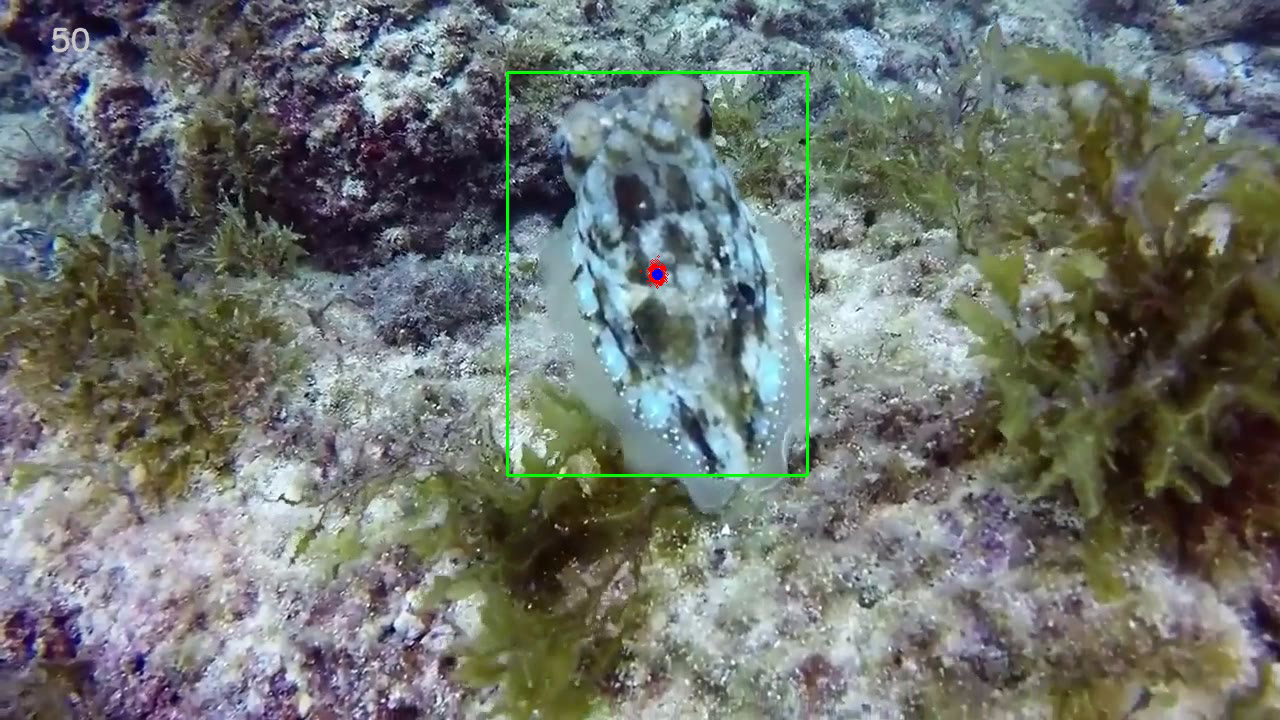
\includegraphics[scale=0.15]{result_pf_valid_2.png}}}
	\\
	\subfloat[Frame 100]{{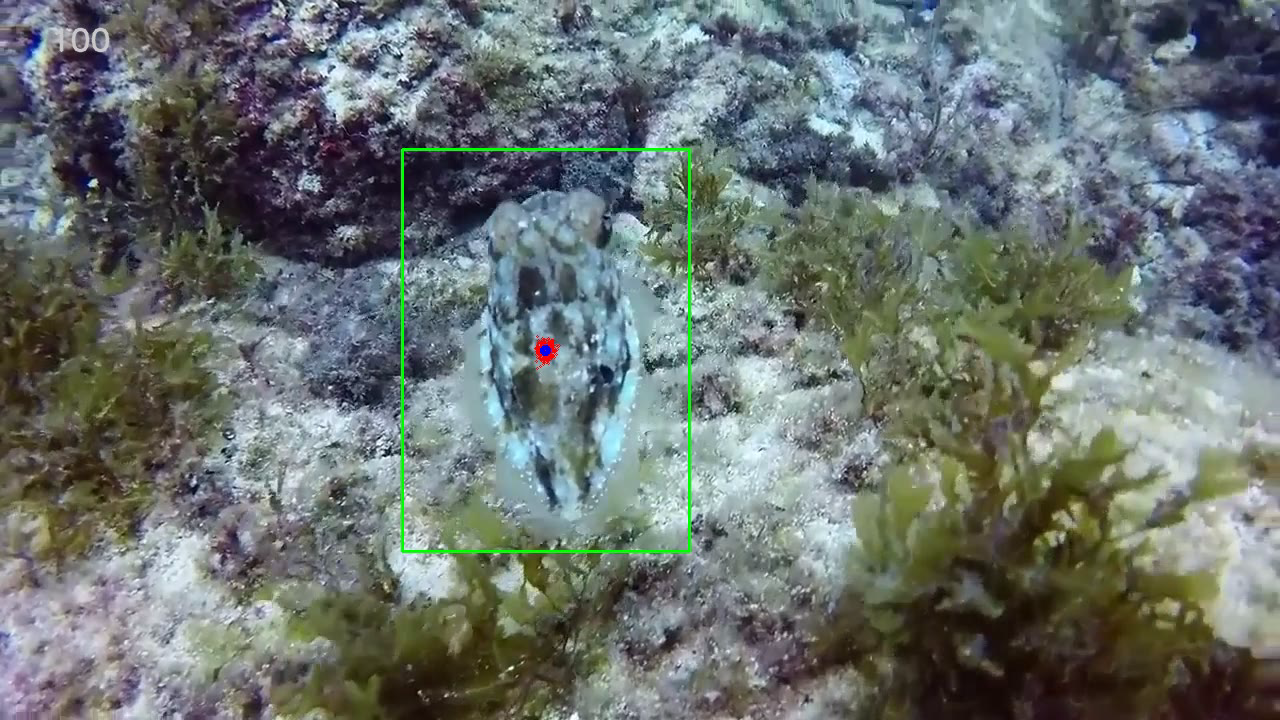
\includegraphics[scale=0.15]{result_pf_valid_3.png}}}
	\hspace{0.1cm}
	\subfloat[Frame 150]{{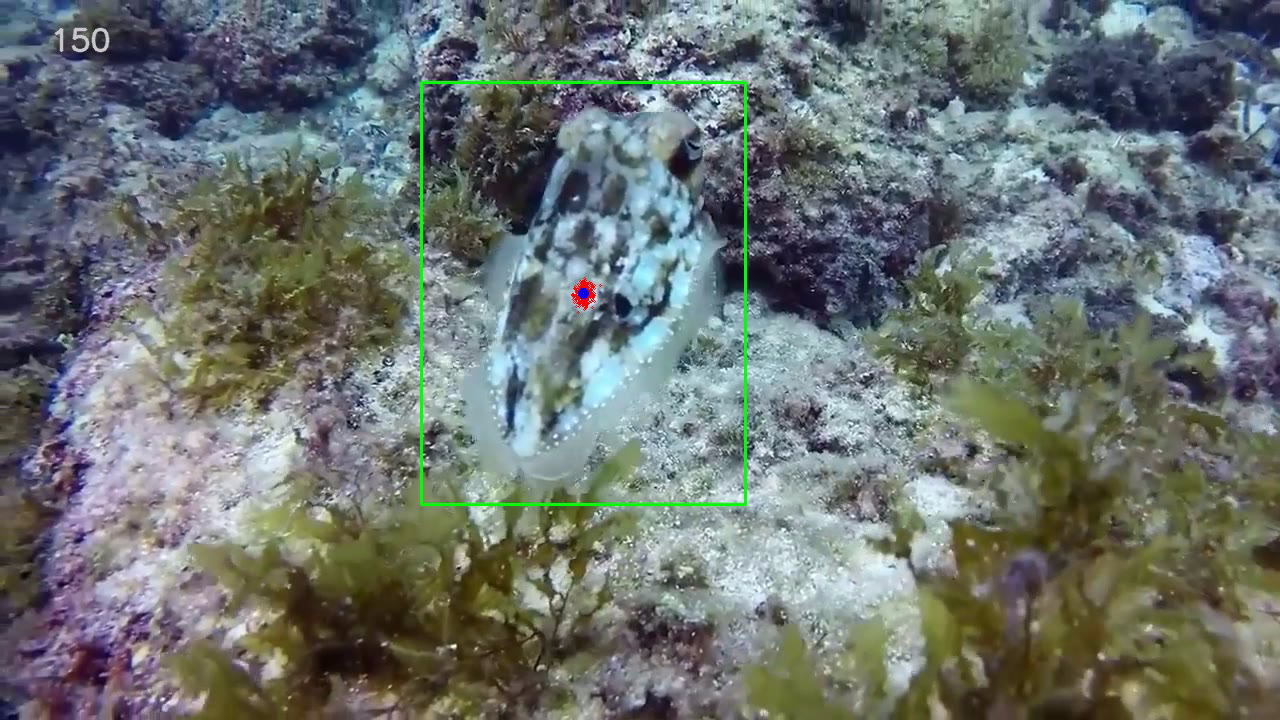
\includegraphics[scale=0.15]{result_pf_valid_4.png}}}
	\\
	\subfloat[Frame 200]{{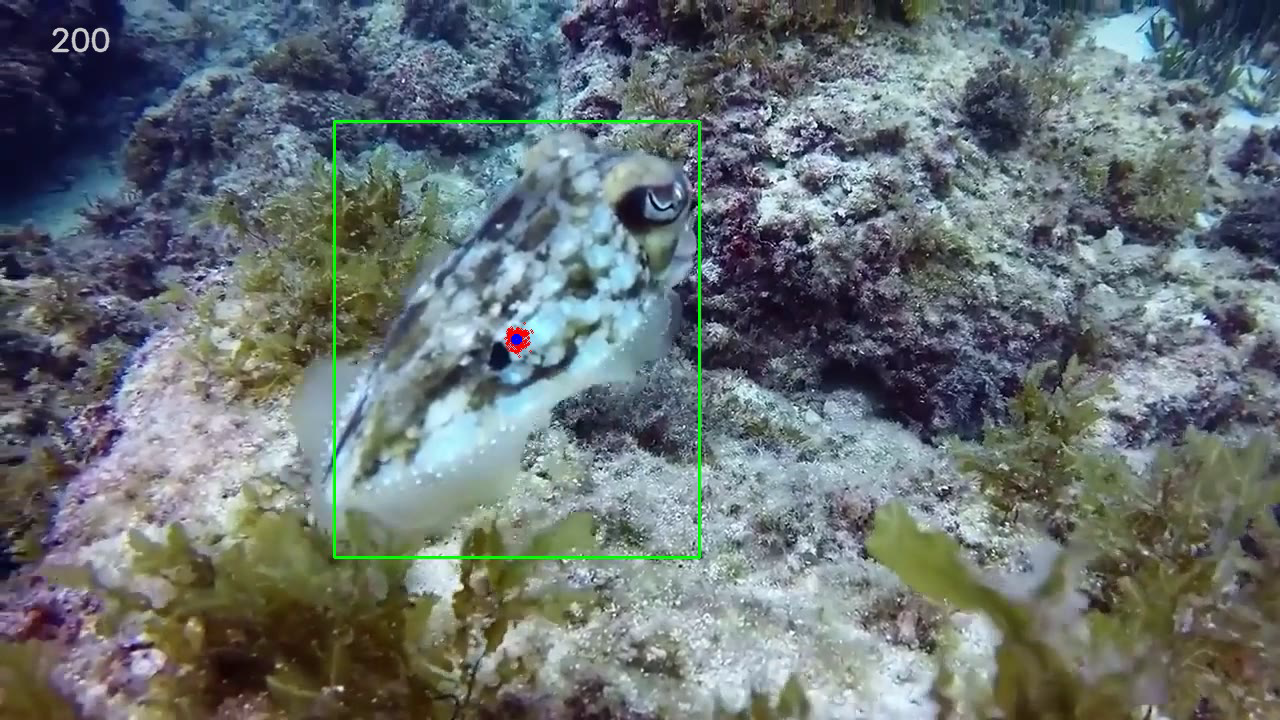
\includegraphics[scale=0.15]{result_pf_valid_5.png}}}
	\hspace{0.1cm}
	\subfloat[Frame 250]{{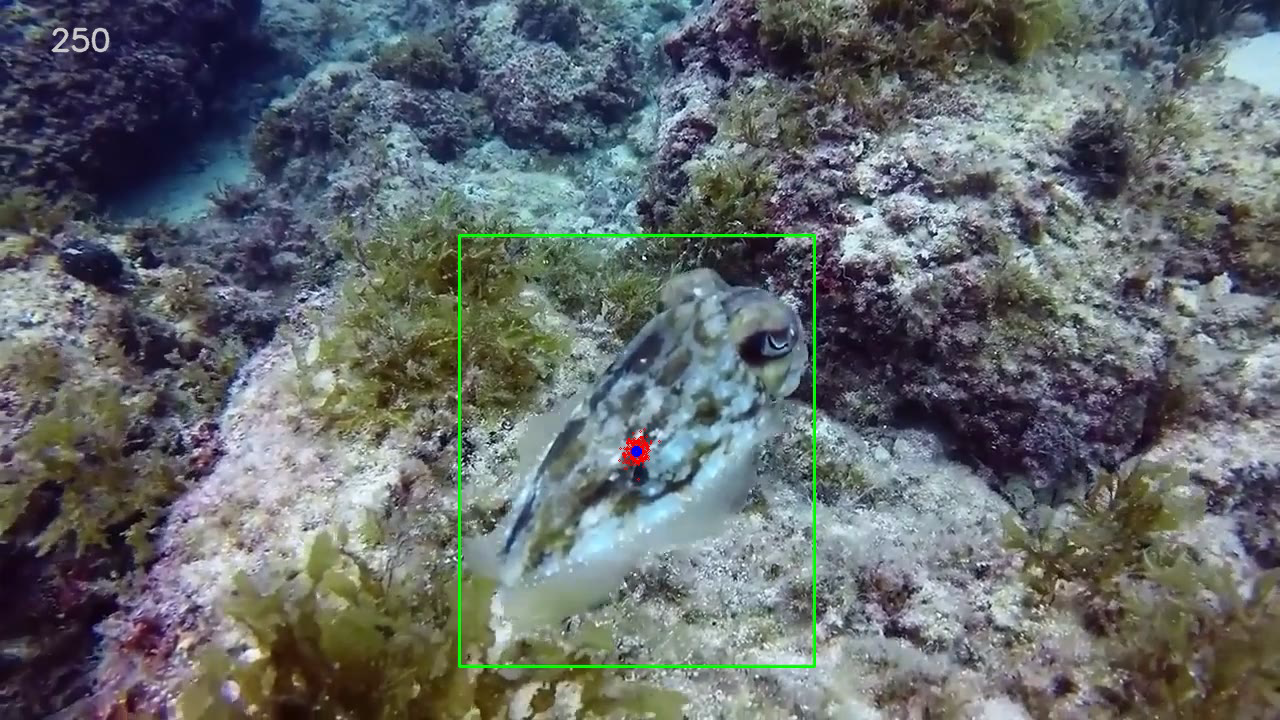
\includegraphics[scale=0.15]{result_pf_valid_6.png}}}
\caption{Exemple de résultats obtenus par notre filtre à particule.}
\label{fig:pf_results}
\end{figure}
\FloatBarrier

\begin{figure}[!htbp]
\center
	\subfloat[Frame 25]{{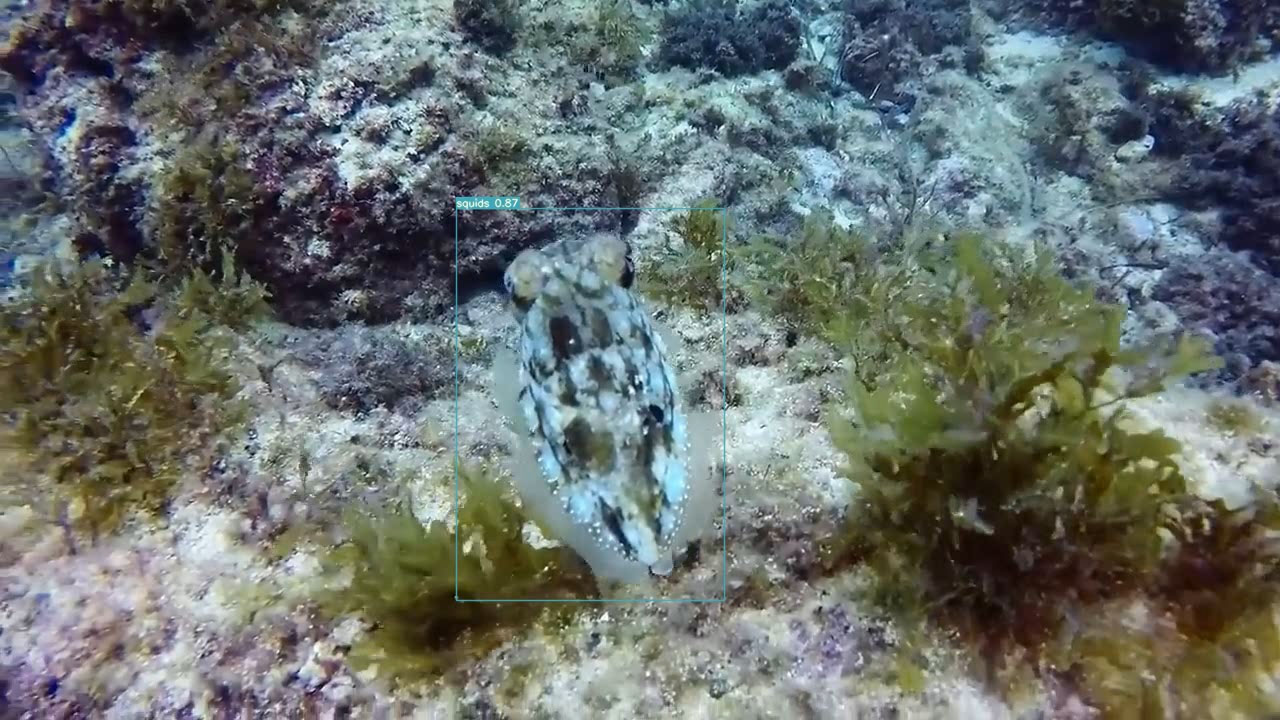
\includegraphics[scale=0.15]{result_yolo_valid_1.jpg}}}
	\hspace{0.1cm}
	\subfloat[Frame 50]{{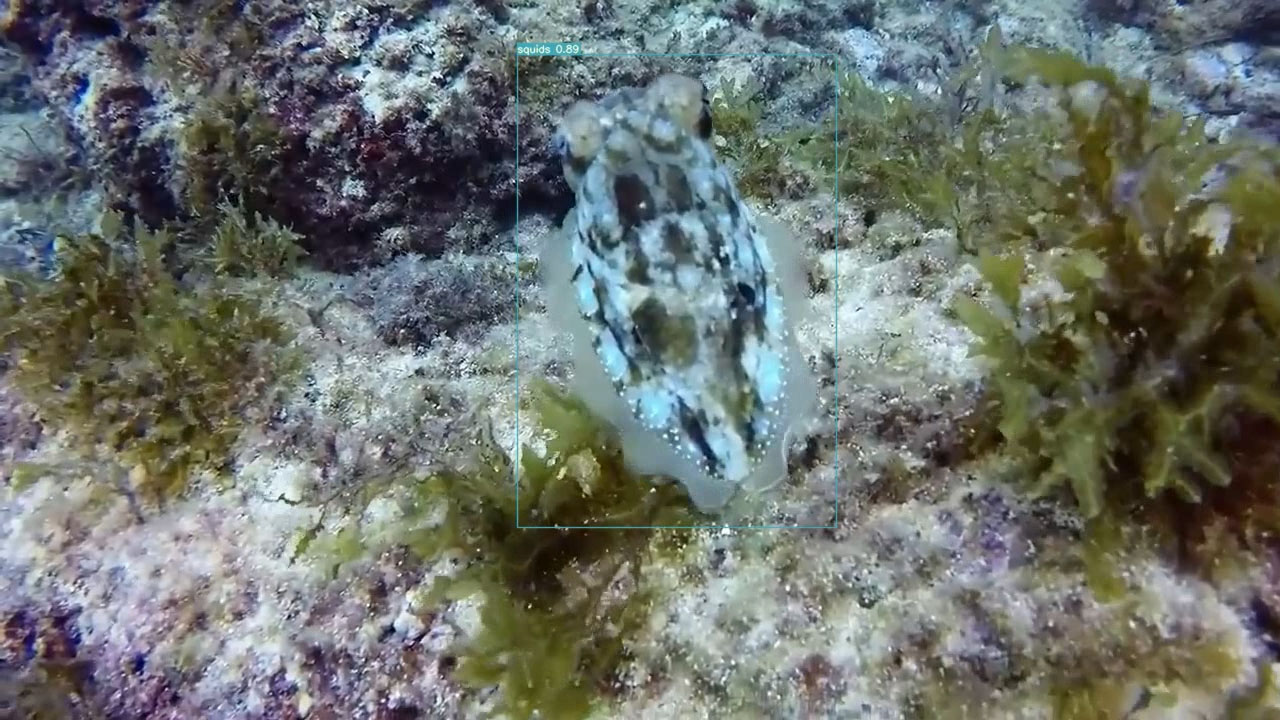
\includegraphics[scale=0.15]{result_yolo_valid_2.jpg}}}
	\\
	\subfloat[Frame 100]{{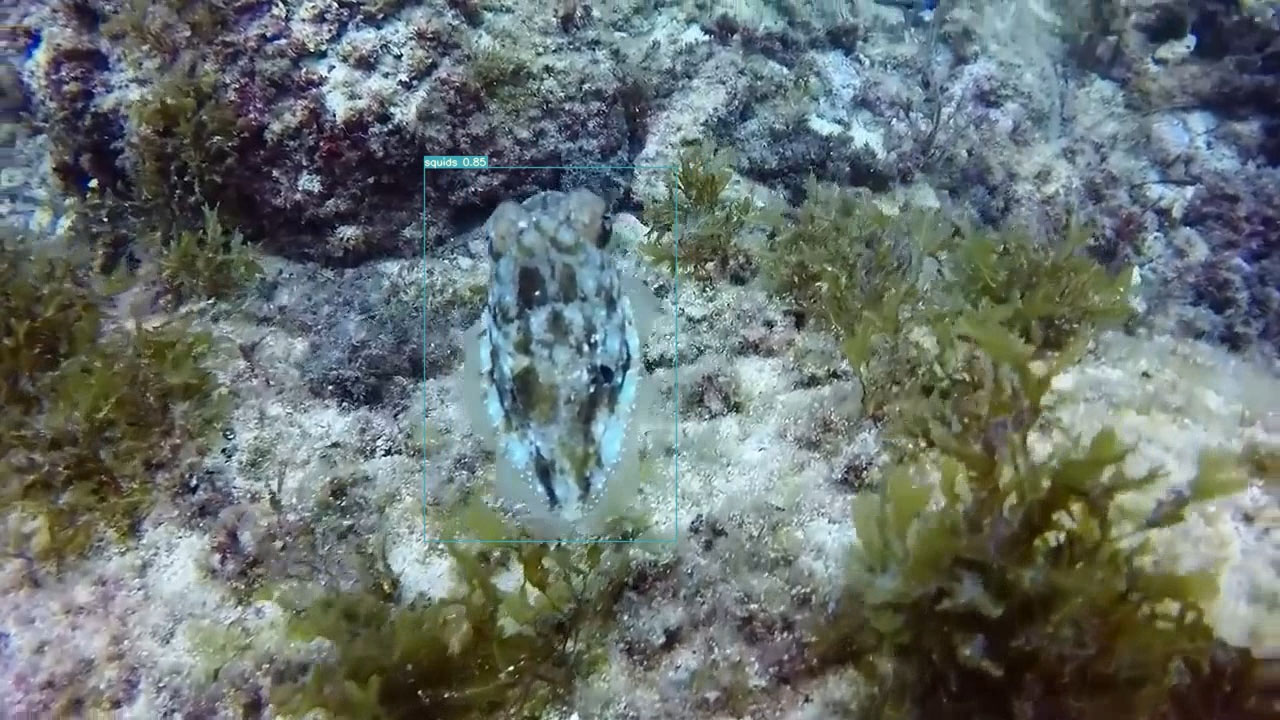
\includegraphics[scale=0.15]{result_yolo_valid_3.jpg}}}
	\hspace{0.1cm}
	\subfloat[Frame 150]{{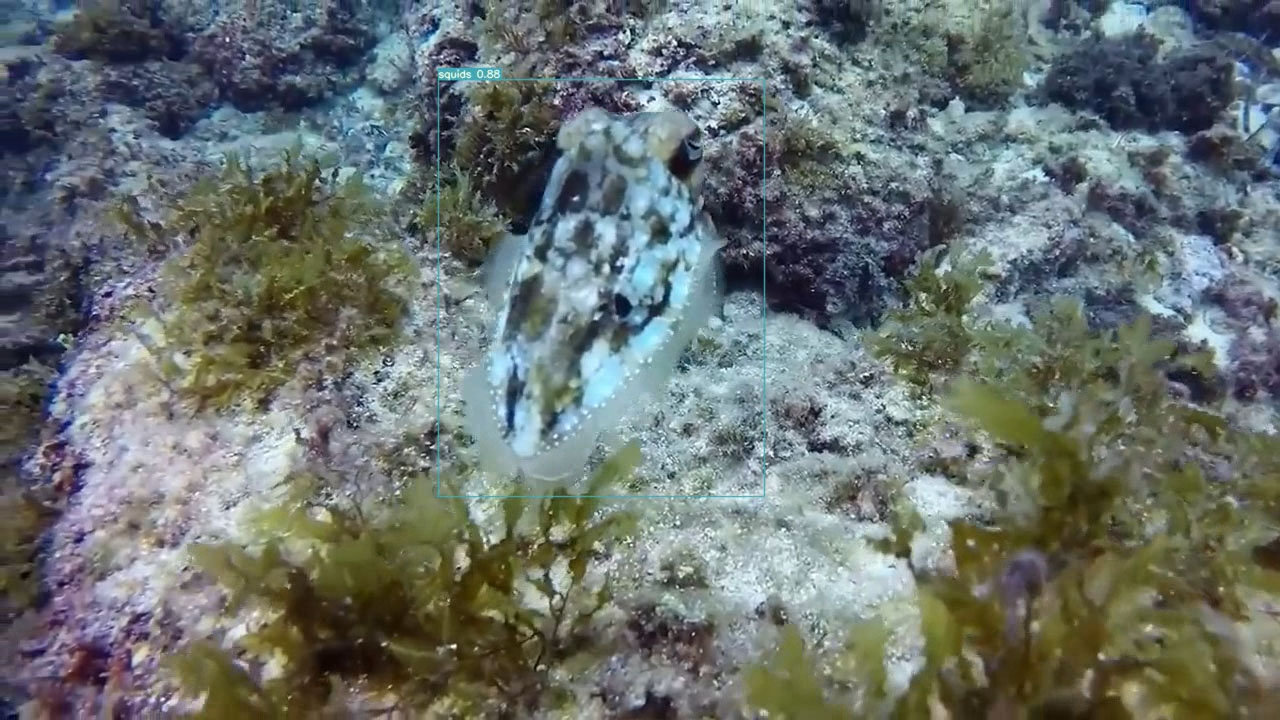
\includegraphics[scale=0.15]{result_yolo_valid_4.jpg}}}
	\\
	\subfloat[Frame 200]{{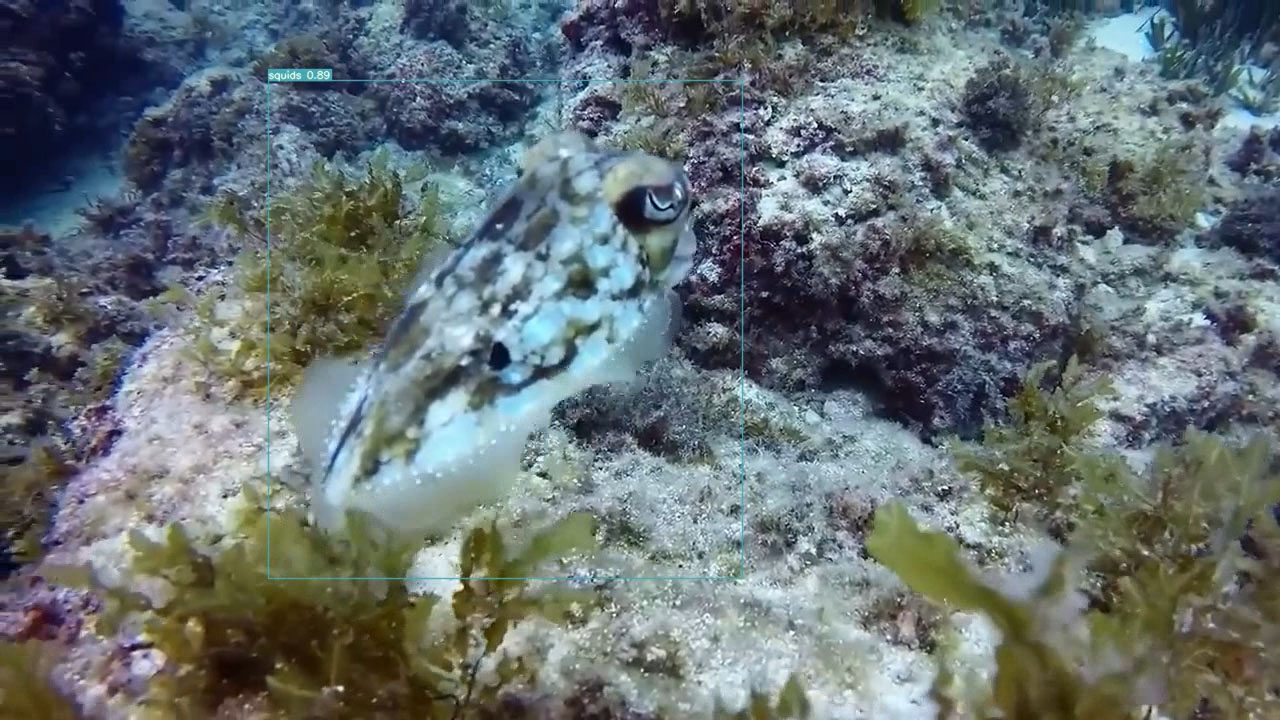
\includegraphics[scale=0.15]{result_yolo_valid_5.jpg}}}
	\hspace{0.1cm}
	\subfloat[Frame 250]{{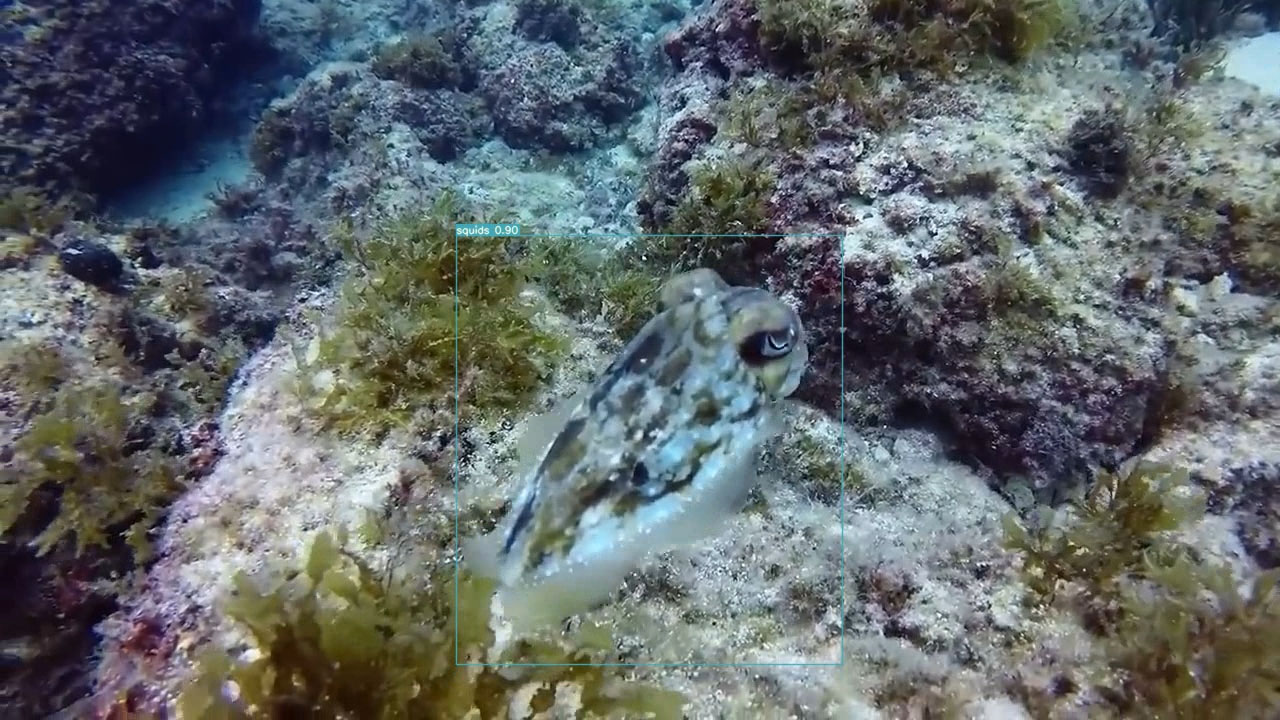
\includegraphics[scale=0.15]{result_yolo_valid_6.jpg}}}
\caption{Exemple de résultats obtenus par YOLOv7.}
\label{fig:yolo_results}
\end{figure}
\FloatBarrier

Les courbes de déplacement de la seiche dans les figure \ref{fig:trajX_pf}, \ref{fig:trajY_pf}, \ref{fig:trajX_yolo} et \ref{fig:trajY_yolo} illustre un exemple de détection continue dans une séquence.\\
Dans la figure \ref{fig:trajX_pf}, nous comparons la trajectoire de la seiche suivi par le filtre à particule (couleur violette) aux positions définies manuellement (couleur or) dans la direction des x, tandis que dans la figure \ref{fig:trajY_pf} nous comparons les deux trajectoires dans la direction des y.\\
De même, dans la figure \ref{fig:trajX_yolo} nous comparons la trajectoir de la seiche suivi par YOLOv7 (couleur bleu) aux positions définies manuellement (couleur or) dans la direction des x, tandis que dans la figure \ref{fig:trajY_yolo} nous comparons les deux trajectoires dans la direction des y.\\
\\
La distance entre la trajectoire automatique et manuelle indique la précision de l'algorithme, ce qui donne pour la séquence une erreur moyenne globale de 21 pixels pour le filtre à particule, calculé sur les 288 frames de la séquence où la seiche a été détecté, et 12 pixels pour YOLOv7, calculé sur les 292 frames de la séquence où la seiche a été détecté.\\
La méthode de détection avec filtre à particule semble détecter la seiche dans 98\% de la séquence, et la méthode de détection avec YOLOv7 dans 100\% de la séquence.

\begin{figure}[!htbp]
\center
	\subfloat{{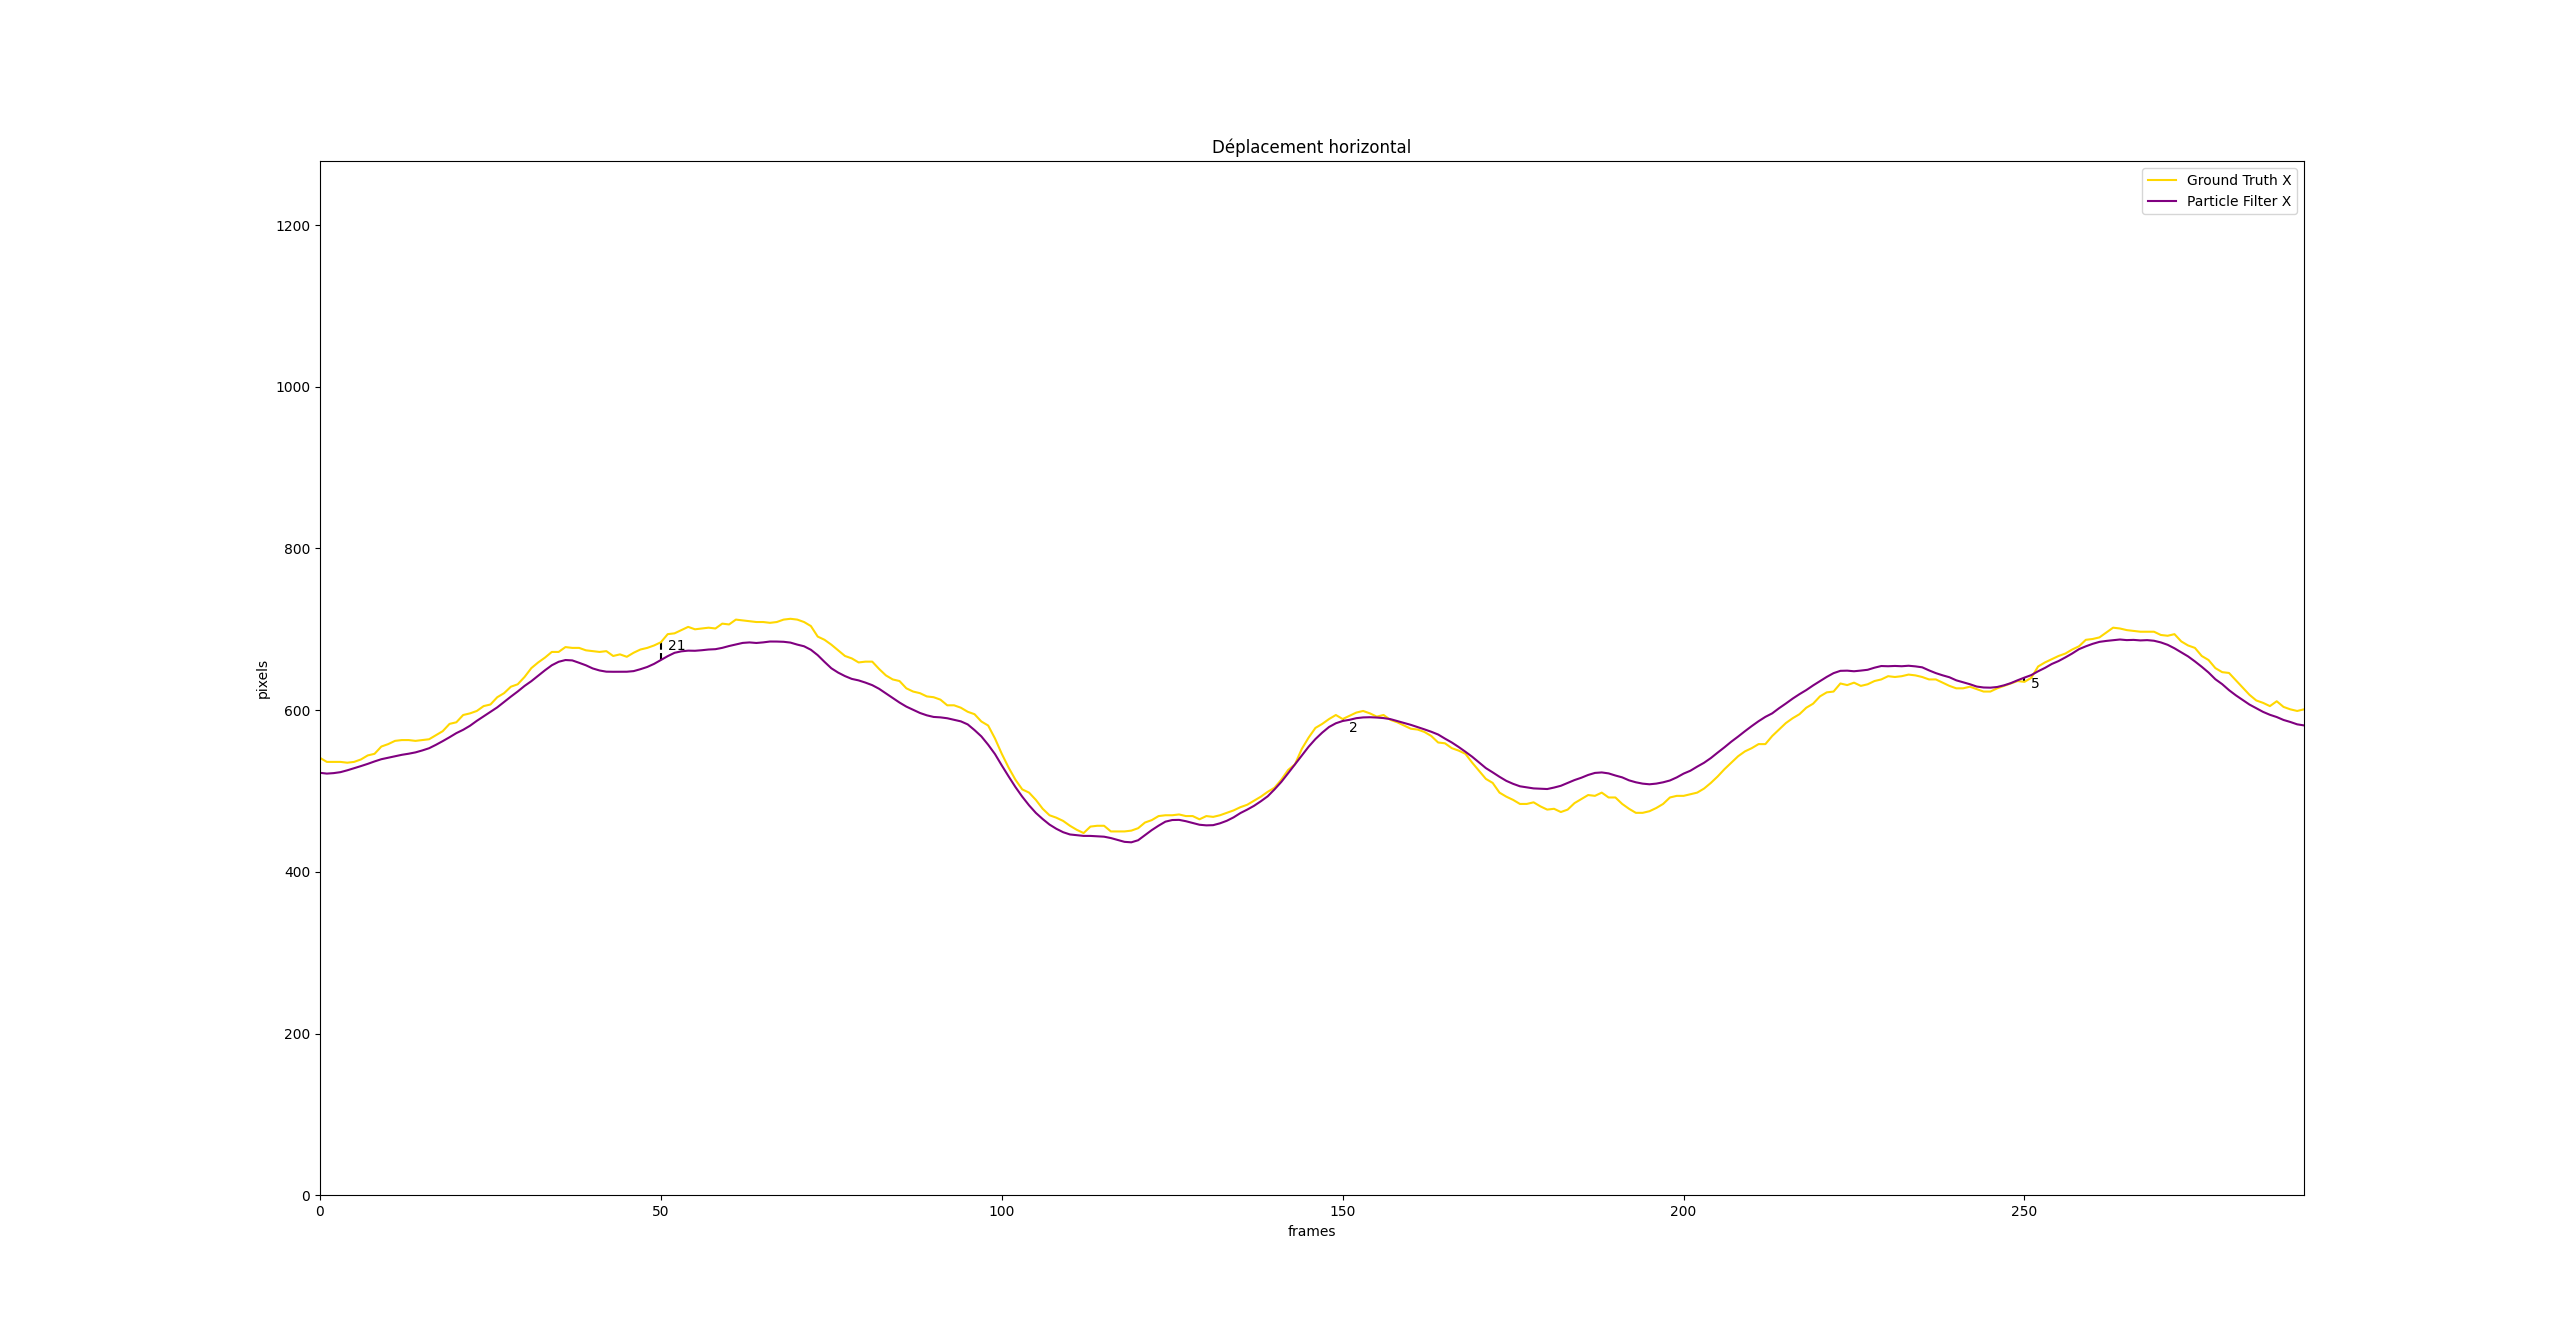
\includegraphics[scale=0.3]{X_displacement_pf.png}}}
\caption{Trajectoire avec le filtre à particule sur les X}
\label{fig:trajX_pf}
\end{figure}
\FloatBarrier

\begin{figure}[!htbp]
\center
	\subfloat{{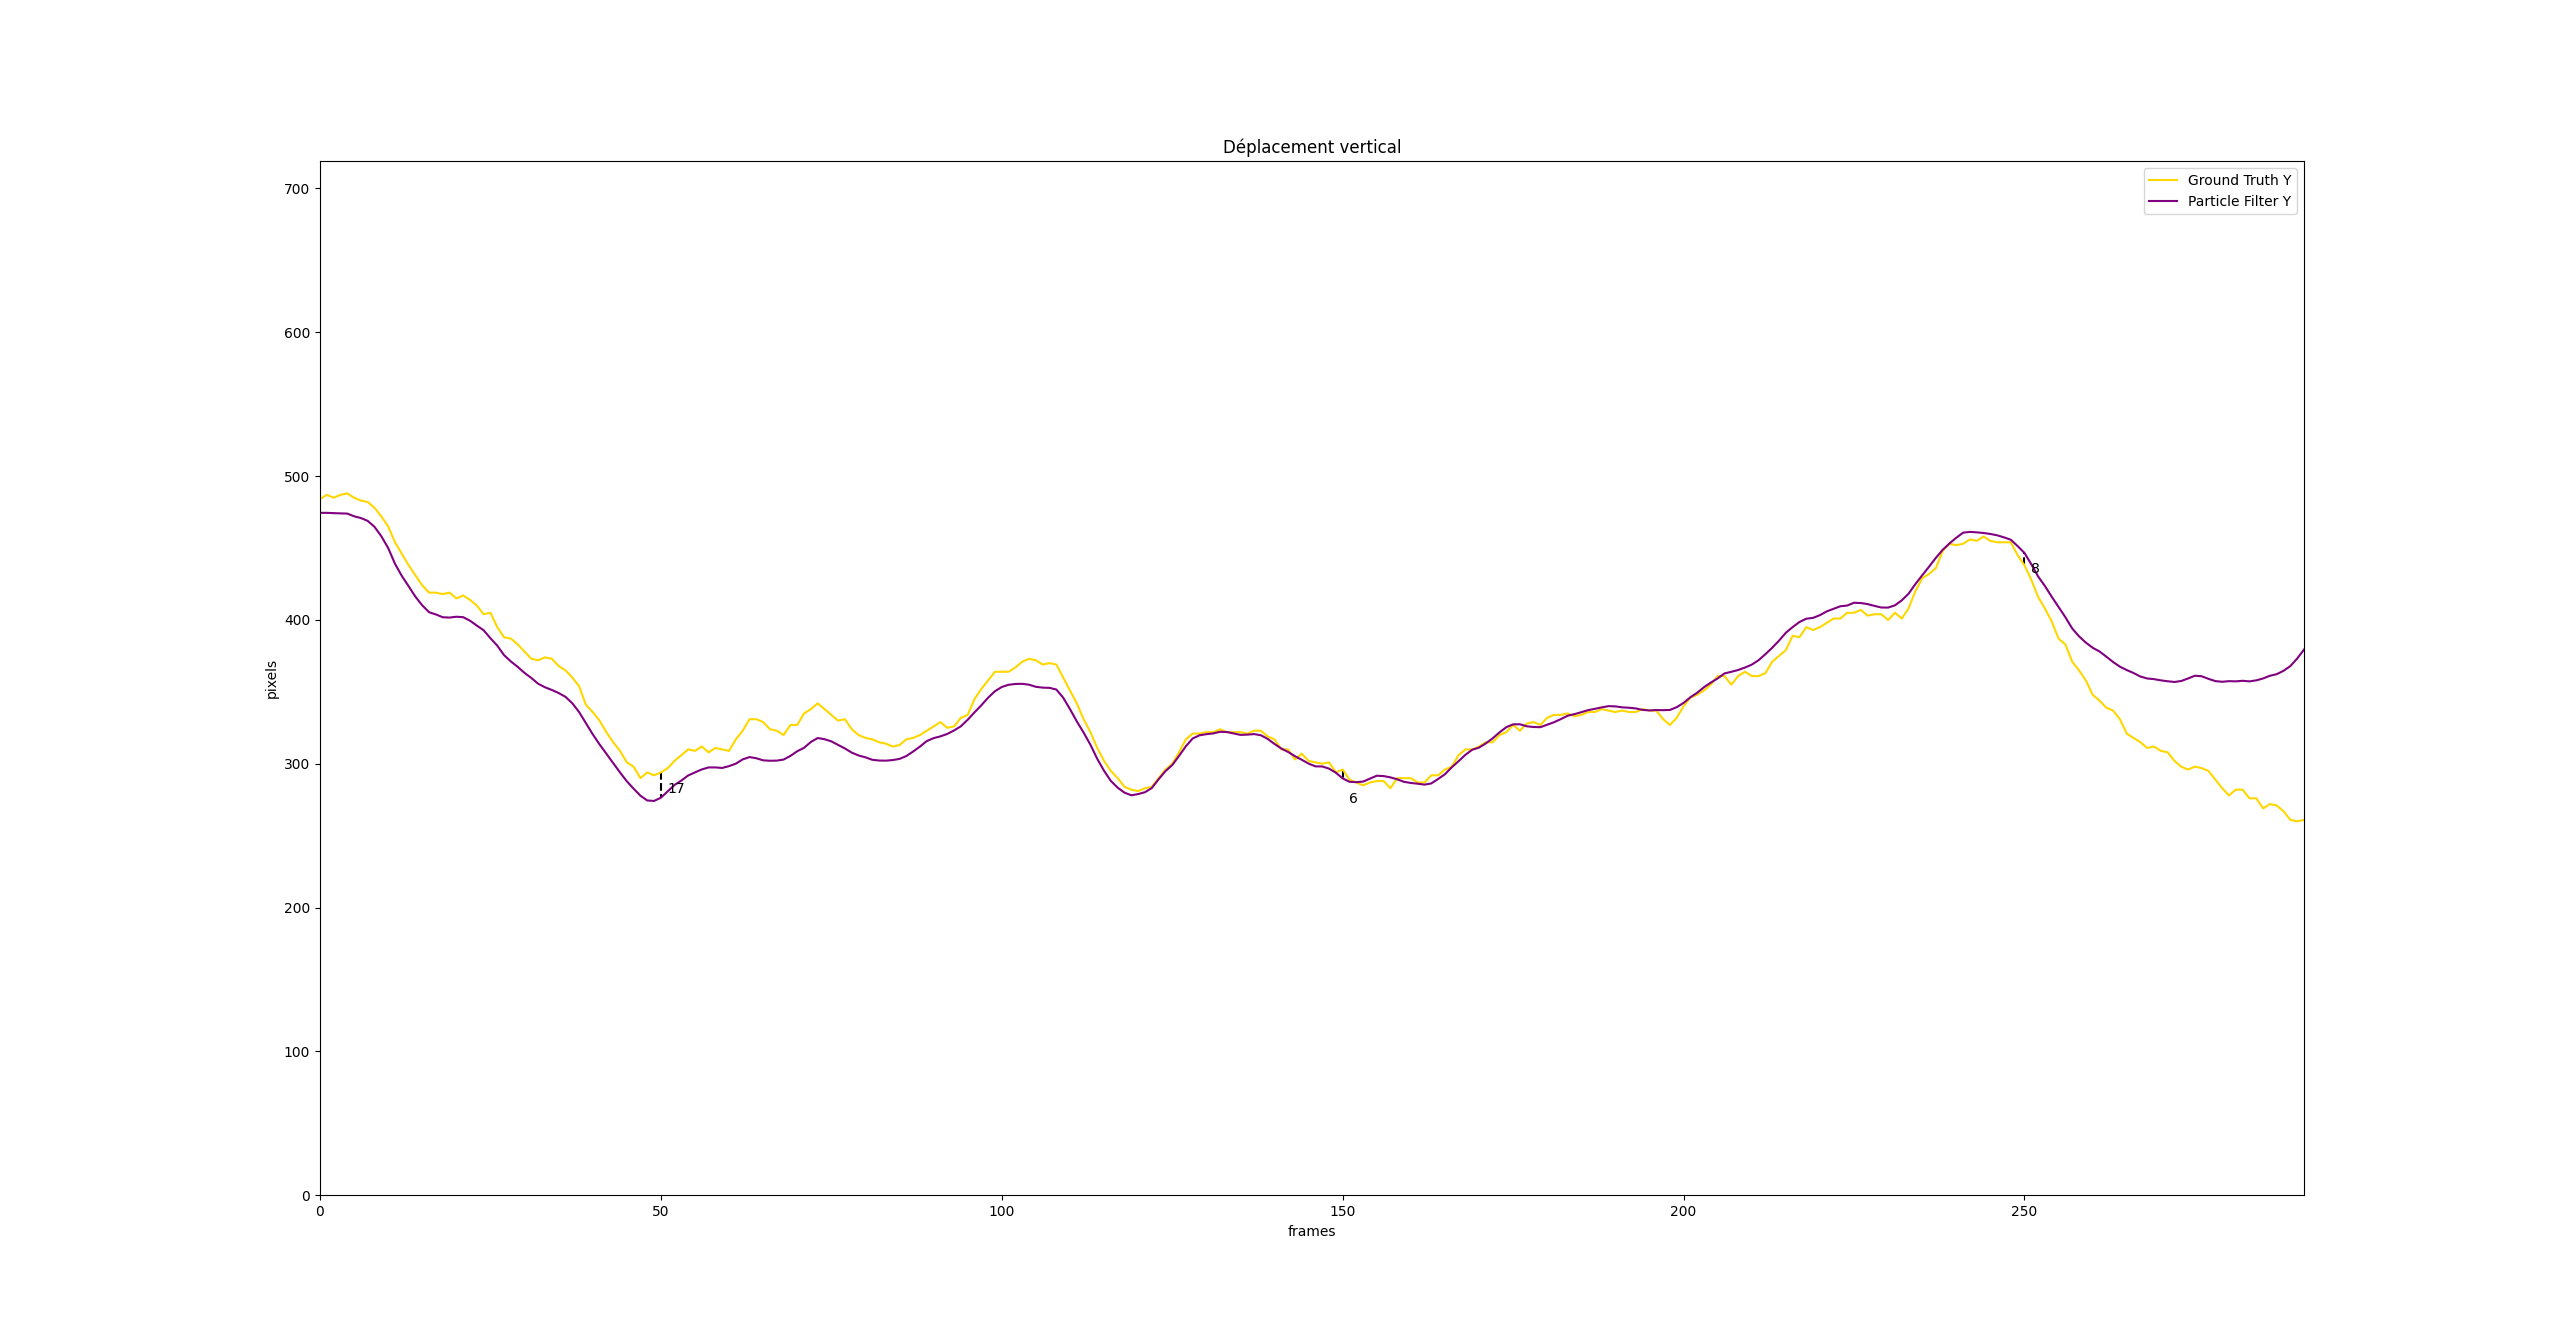
\includegraphics[scale=0.3]{Y_displacement_pf.png}}}
\caption{Trajectoire avec le filtre à particule sur les Y}
\label{fig:trajY_pf}
\end{figure}
\FloatBarrier

\begin{figure}[!htbp]
\center
	\subfloat{{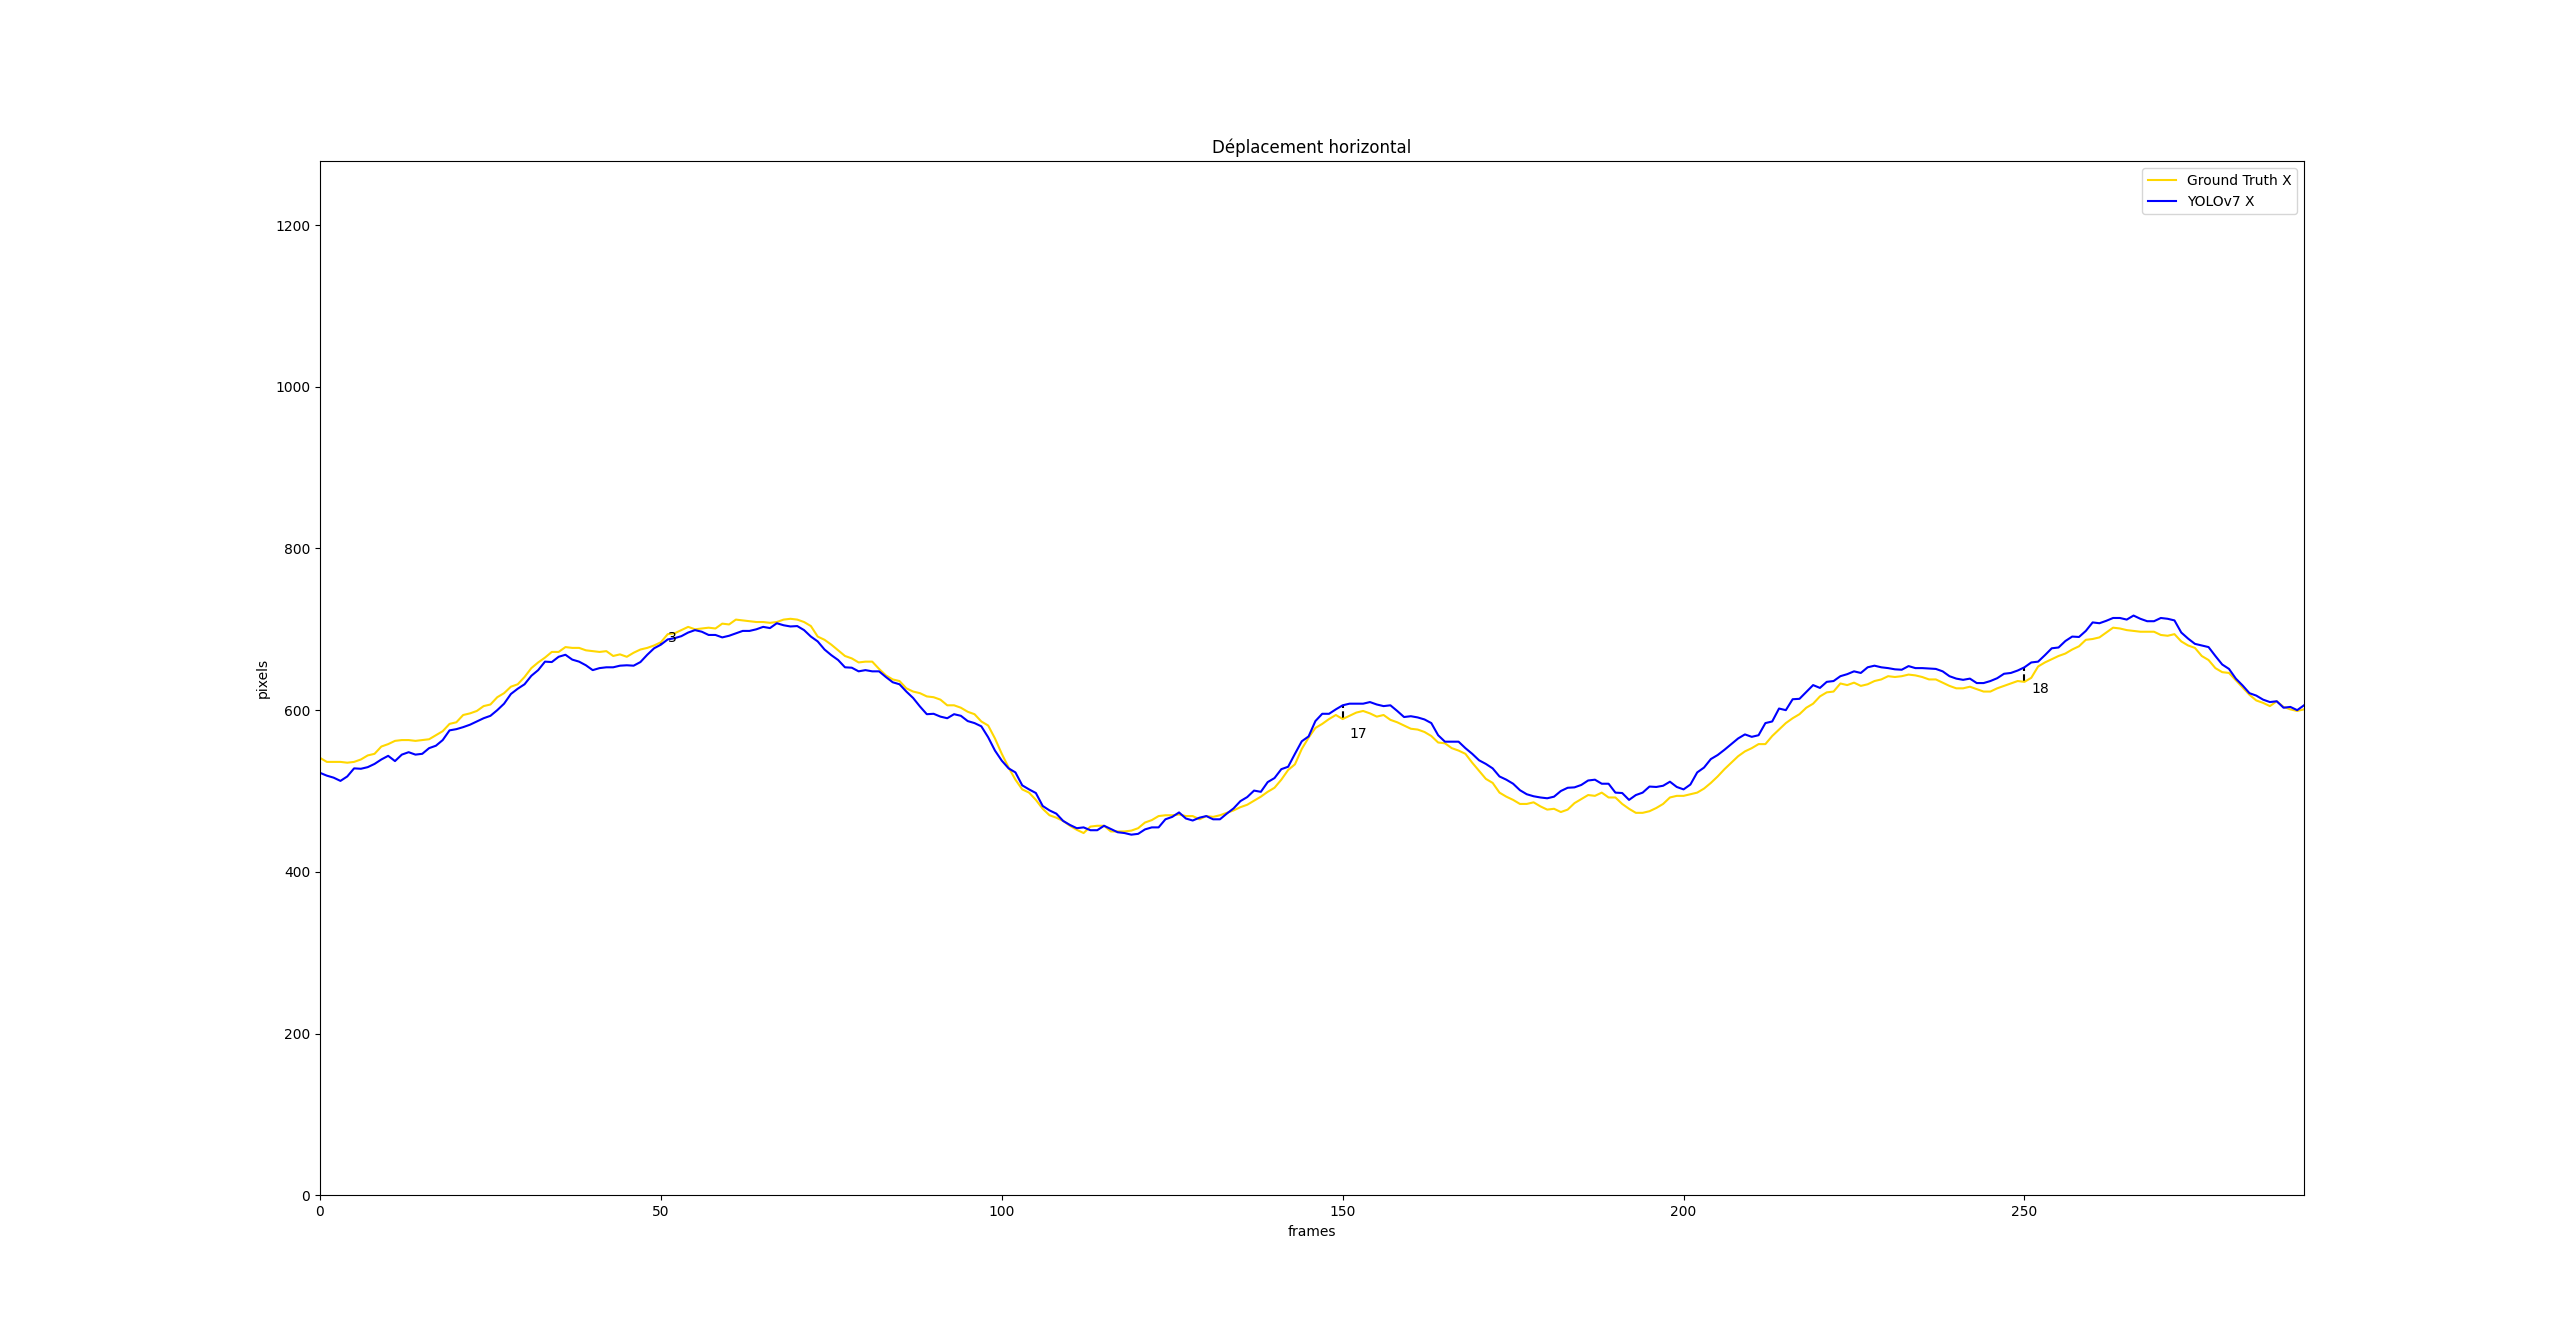
\includegraphics[scale=0.3]{X_displacement_yolo.png}}}
\caption{Trajectoire avec YOLOv7 sur les X}
\label{fig:trajX_yolo}
\end{figure}
\FloatBarrier

\begin{figure}[!htbp]
\center
	\subfloat{{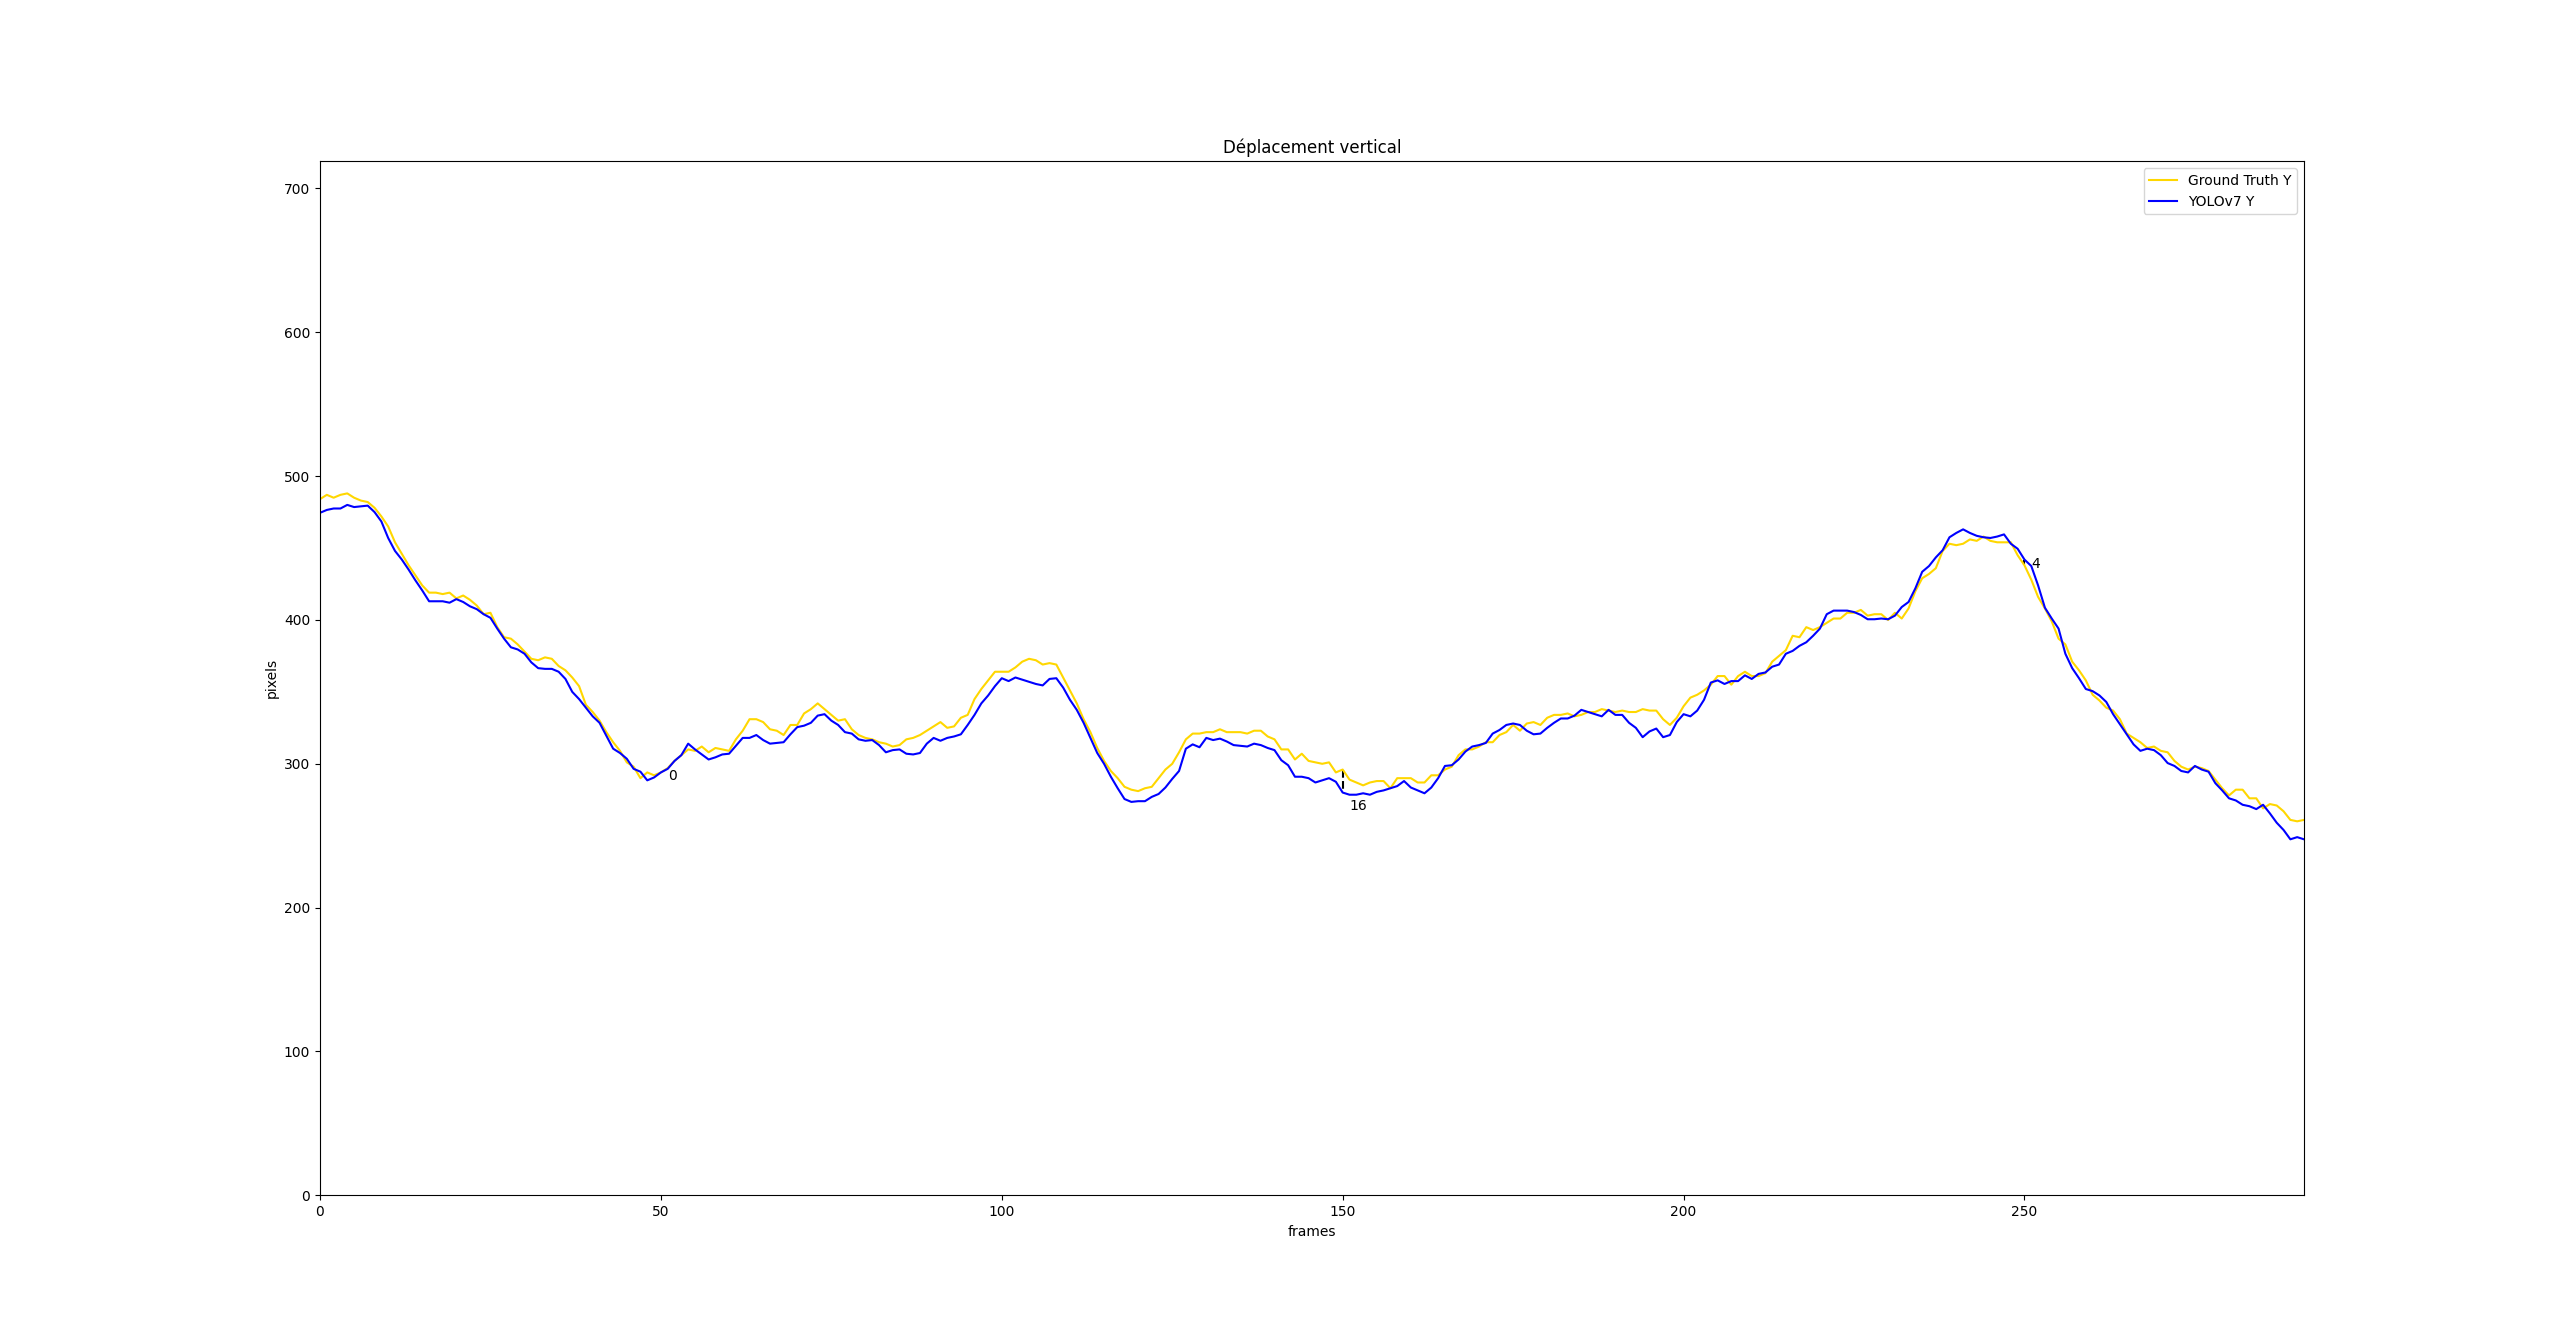
\includegraphics[scale=0.3]{Y_displacement_yolo.png}}}
\caption{Trajectoire avec YOLOv7 sur les Y}
\label{fig:trajY_yolo}
\end{figure}
\FloatBarrier
 
Cependant, la détection avec le filtre à particule peut diverger, comme illustré dans la figure \ref{fig:pf_diverg_results}. Cette divergence peut s'expliquer de plusieurs manières, elle peut provenir d'une accumulation d'erreur lors du suivi, ou bien d'une paramétrisation du logiciel non optimale, ou encore de la seiche qui n'est que sur une petite portion de la bounding box, ce qui a pour effet de beaucoup plus représenter l'arrière plan et donc mettre un poids plus élevé sur ce qui ressemble à l'arrière plan lors de l'étape de calcul des poids.

\begin{figure}[!htbp]
\center
	\subfloat{{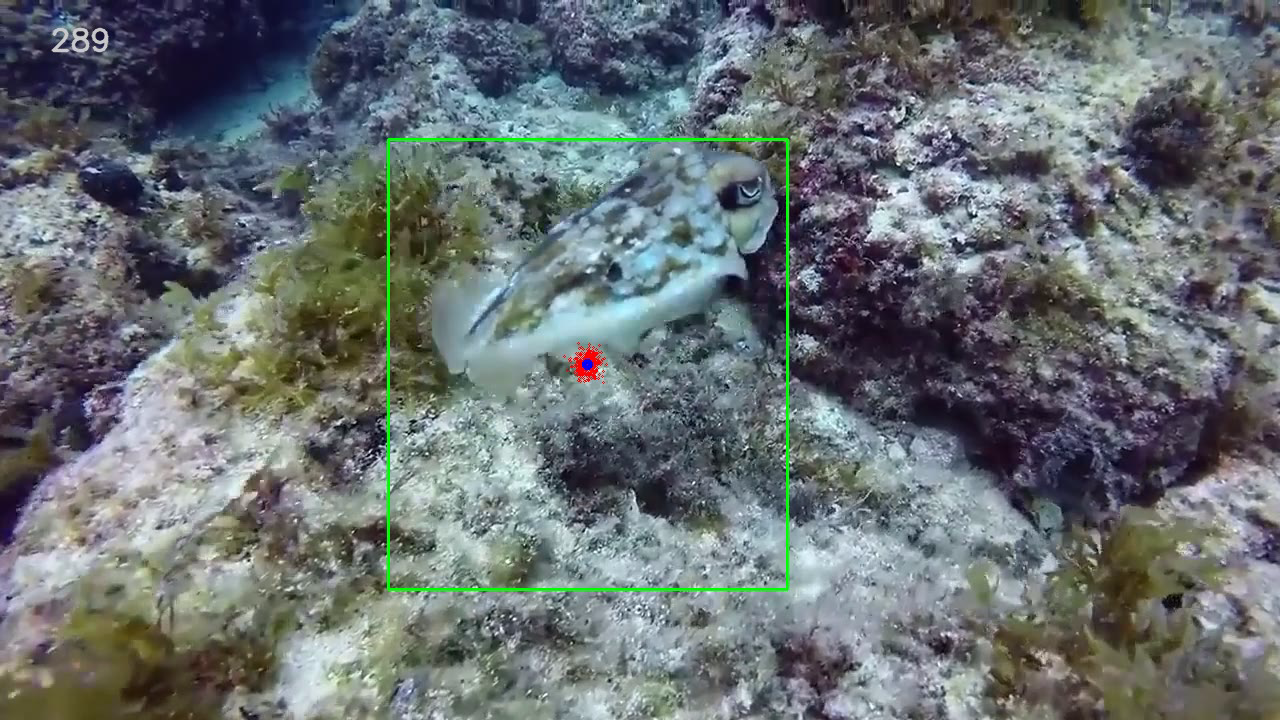
\includegraphics[scale=0.15]{result_pf_invalid_1.png}}}
	\hspace{0.1cm}
	\subfloat{{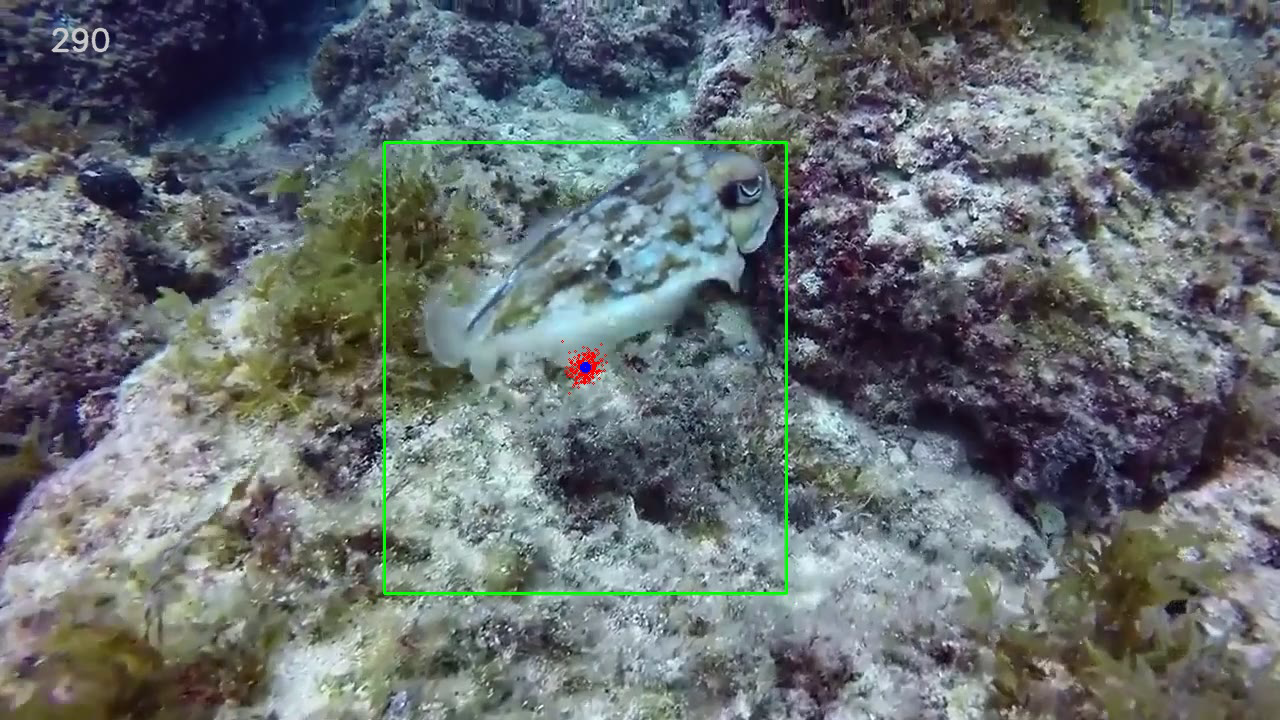
\includegraphics[scale=0.15]{result_pf_invalid_2.png}}}
	\\
	\subfloat{{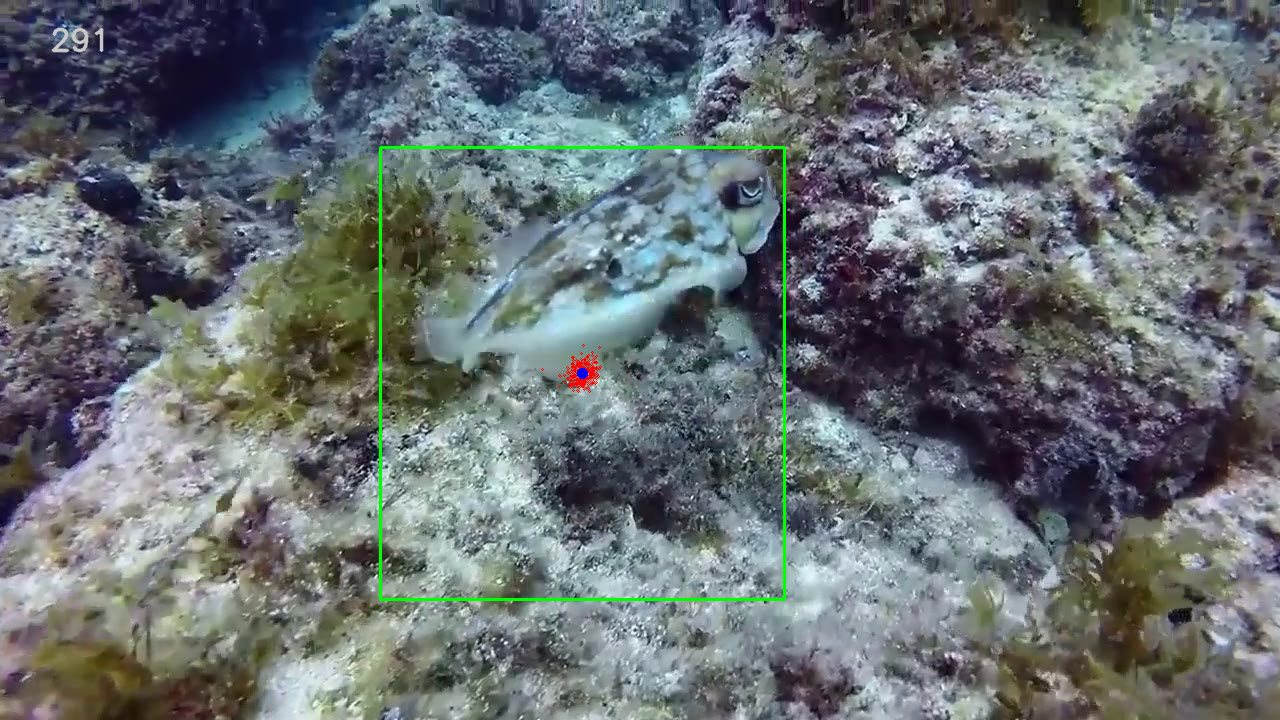
\includegraphics[scale=0.15]{result_pf_invalid_3.png}}}
	\hspace{0.1cm}
	\subfloat{{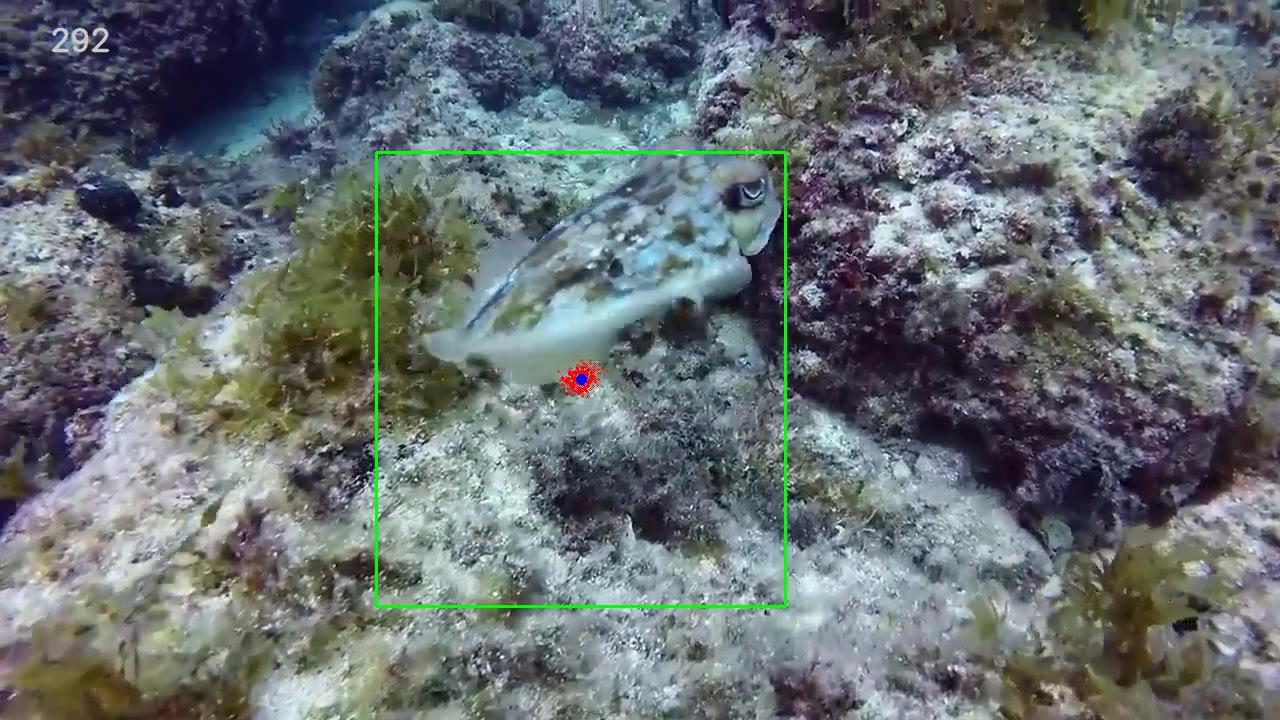
\includegraphics[scale=0.15]{result_pf_invalid_4.png}}}
\caption{Exemple de résultats divergeant obtenus par notre filtre à particule.}
\label{fig:pf_diverg_results}
\end{figure}
\FloatBarrier

\clearpage

\chapter{Gestion du Projet}

\section{Planification}

\section{Changements majeurs}

\clearpage

\pagestyle{plain}
\chapter{Bilan et Conclusions}
Au terme de ce projet, nous disposons d'un logiciel de suivi de seiche en milieu aquatique non contrôlé, qui peut utiliser différentes combinaisons de descripteurs et de mesures de similarité.\\
Les résultats montrent que sur des vidéos prises en conditions réelles, et avec une configuration du logiciel adéquate, le suivi se fait avec une efficacité d'environ 75\% par rapport aux données de référence. Ce résultat est très satisfaisant et n'a qu'une différence de 1\% avec la méthode qui utilise uniquement YOLOv7.\\
Cependant, notre méthode reste très dépendante de la configuration donnée par l'utilisateur, ainsi qu'aux caractéristiques des vidéos, comme le mouvement de la caméra, le contraste, la luminosité, ou encore l'arrière plan qui peut prendre une trop grande proportion dans la bounding box et faire diverger le suivi. Mais, avec une configuration adéquate, nous arrivons à obtenir un suivi satisfaisant pour les cas problématiques définis dans l'\hyperlink{chapter.1}{introduction}, comme par exemple les mouvements de la caméra ou la déformation de la seiche au cours de la vidéo.\\
\\
Les perspectives d'amélioration tournent principalement autour des réseaux de neurones et du temps réel.\\
En effet, le suivi actuel se fait en post-processing et peut demander un certain temps en fonction de la configuration donnée au logiciel. On pourrait donc essayer d'accélérer et d'améliorer le suivi en combinant l'algorithme du filtre à particule avec des réseaux de neurones, ou bien utiliser exclusivement des réseaux de neurones.\\
\\
On pourrait par exemple entrainer un VAE (\ref{app:variational_autoencoder}) sur des images de seiches, et récupérer la partie encodeur du VAE pour l'utiliser comme un descripteur à la place de HOG. En faisant cela, on s'assure que le vecteur descripteur sortant de l'encodeur représente bien l'image que l'on a donnée en entrée.\\
\\
On pourrait également utiliser uniquement des réseaux de neurones, comme YOLOv7 qui a prouvé son efficacité dans la partie \hyperlink{chapter.5}{5} et qui traite chaque image en environ 2ms, ce qui est amplement suffisant pour faire du temps réel.

\clearpage


% Exemple de reference
\cite{xu_human_2010}
\cite{kong_particle_2019}
\cite{qiang_zhu_fast_2006}
\cite{dalal_histograms_2005}
\cite{bhattacharyya_measure_1960}
\cite{rlabbe}


\printbibliography

\begin{appendices}
	
\section*{mAP (mean Average Precision)}\label{app:mAP}
La mAP est une mesure de précision pour les algorithmes de détection d'objet. La mAP correspond de manière générale à la moyenne de l'AP obtenu sur différents objets et à différents paramètres. Son calcul dépend du contexte et de la technique de comparaison.\\
L'Average Precision (AP) se calcule en se basant sur la précision, le rappel et l'Intersection over Union. 
\begin{figure}[!htbp]
\center
	\subfloat{{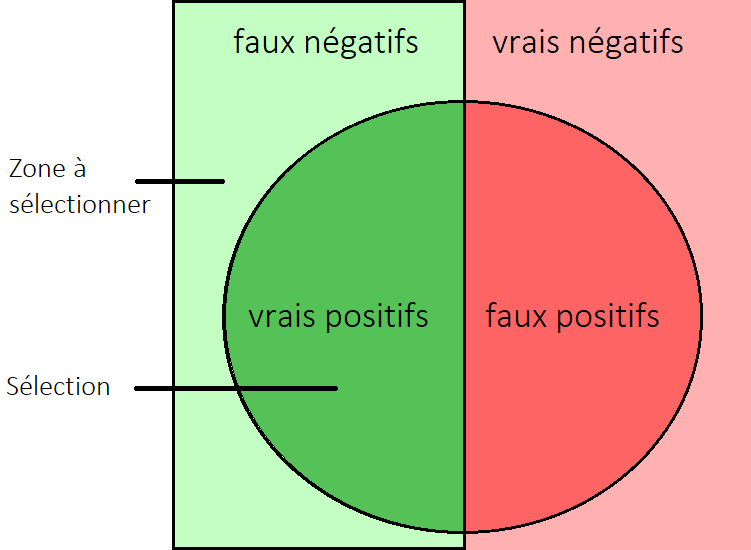
\includegraphics[scale=0.25]{truefalsepositivesnegatives.png}}}
\caption{Schéma vrais/faux positifs/négatifs}
\label{fig:schema_vraifaux}
\end{figure}
\FloatBarrier
La précision correspond à la proportion de vrais positifs (VP) parmi l'ensemble des vrais positifs et des faux positifs (FP). 
$$precision = \frac{VP}{VP+FP}$$
Le rappel correspond à la proportion de vrais positifs parmi l'ensemble des vrais positifs et des faux négatifs (FN).
$$rappel = \frac{VP}{VP+FN}$$
On trace ensuite la courbe représentant la précision en fonction du rappel : 
\begin{figure}[!htbp]
\center
	\subfloat{{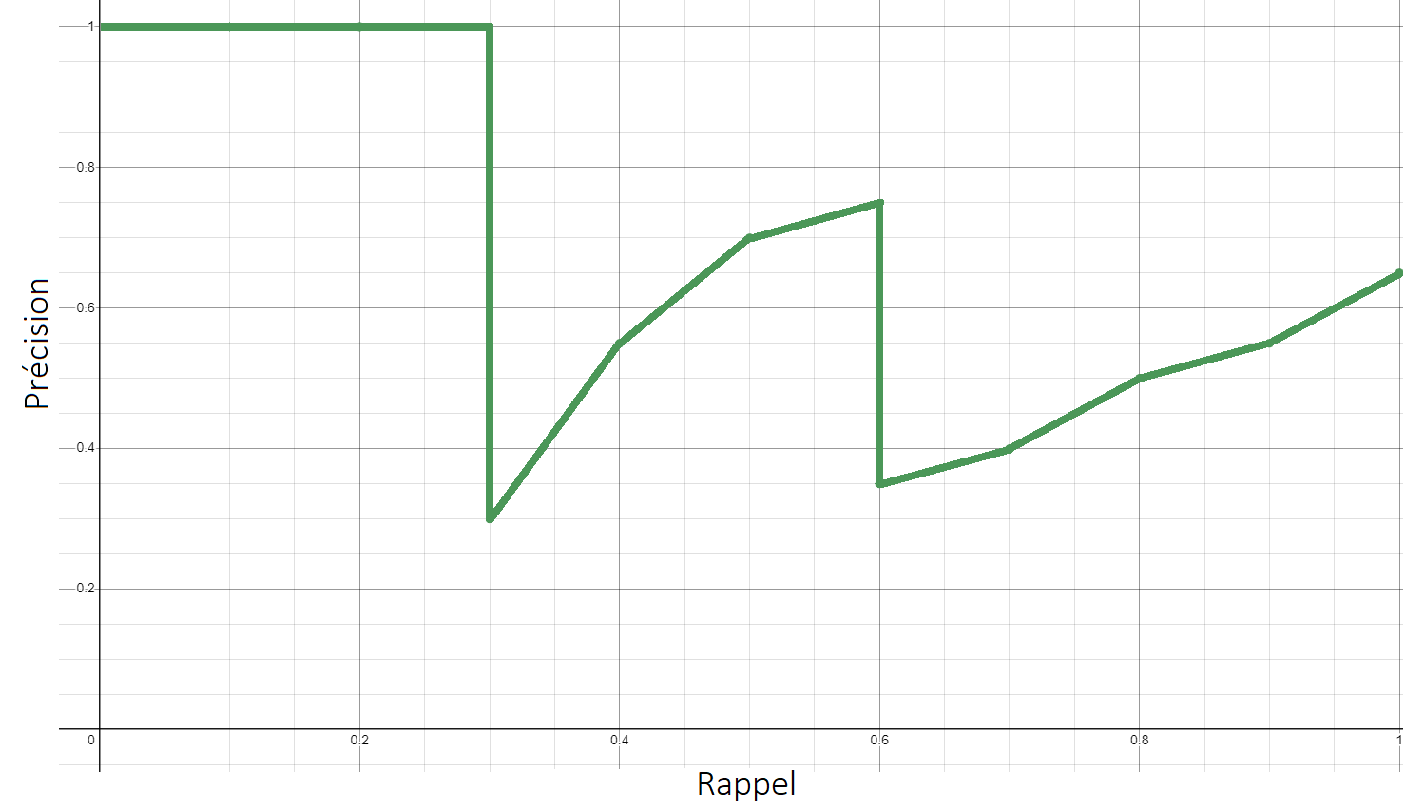
\includegraphics[scale=0.2]{prcurve.png}}}
\caption{Tracé de la coubre Precision-Recall ou PR curve}
\label{fig:trace_prcurve}
\end{figure}
\FloatBarrier
L'AP correspond à l'aire sous cette courbe Precision-Rappel (PR curve). 
$$\int_{0}^{1} f_{PR}(rappel) \hspace{0.1cm} d(rappel)$$

	

	
\clearpage
\section*{Diagramme UML global}\label{app:UMLGlobal}
\begin{figure}[!htbp]
	\center
		\subfloat{{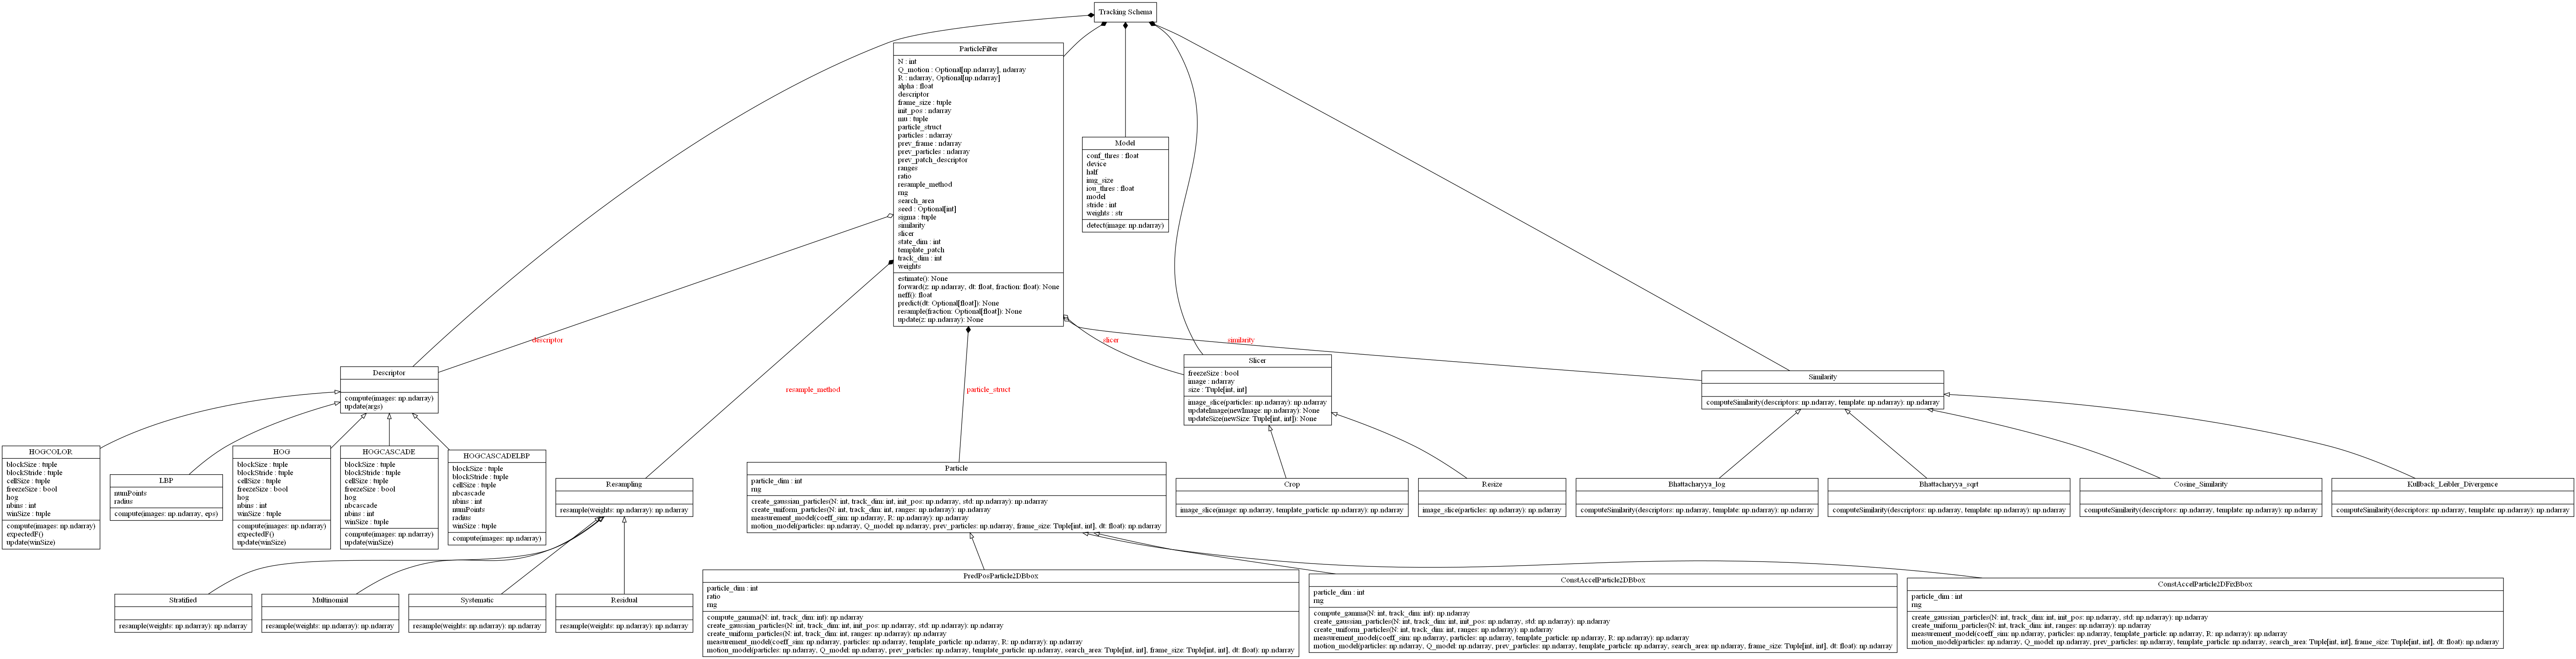
\includegraphics[scale=0.1,angle=90,origin=c]{classes.png}}}
<<<<<<< HEAD
<<<<<<< HEAD
<<<<<<< HEAD
	\caption{Diagramme UML des classes globales (\href{https://raw.githubusercontent.com/gabriel-combe/Cuttlefish_Tracker/main/rapport/UML/classes.svg}{lien vers l'image SVG}, zoomer sur l'image SVG pour avoir plus de détaille).}
=======
	\caption{Diagramme UML des classes globales (\href{https://raw.githubusercontent.com/gabriel-combe/Cuttlefish_Tracker/main/rapport/UML/classes.svg}{lien vers l'image SVG}, zoomer sur l'image SVG pour avoir plus de détails).}
>>>>>>> a979539 (Fix typos)
=======
=======
>>>>>>> c164f46 (Rebase 6/7)
	\caption{Diagramme UML des classes globales (\href{https://raw.githubusercontent.com/gabriel-combe/Cuttlefish_Tracker/main/rapport/UML/classes.svg}{lien vers l'image SVG}, zoomer sur l'image SVG pour avoir plus de détails).}
=======
	\caption{Diagramme UML des classes globales (\href{https://raw.githubusercontent.com/gabriel-combe/Cuttlefish_Tracker/test/rapport/UML/classes.svg}{lien vers l'image SVG}, zoomer sur l'image SVG pour avoir plus de détaille).}
>>>>>>> afae3dc (Change diagram link for SVG)
<<<<<<< HEAD
>>>>>>> 0295ce9 (Rebase 4/7)
=======
=======
	\caption{Diagramme UML des classes globales (\href{https://raw.githubusercontent.com/gabriel-combe/Cuttlefish_Tracker/main/rapport/UML/classes.svg}{lien vers l'image SVG}, zoomer sur l'image SVG pour avoir plus de détaille).}
>>>>>>> f66402e (Fix typos)
>>>>>>> c164f46 (Rebase 6/7)
	\label{fig:uml_diagram_classes}
\end{figure}
\FloatBarrier
	

\clearpage
\section*{Diagramme UML mesure de similarité}\label{app:UMLSimilarity}
\begin{figure}[!htbp]
	\center
		\subfloat{{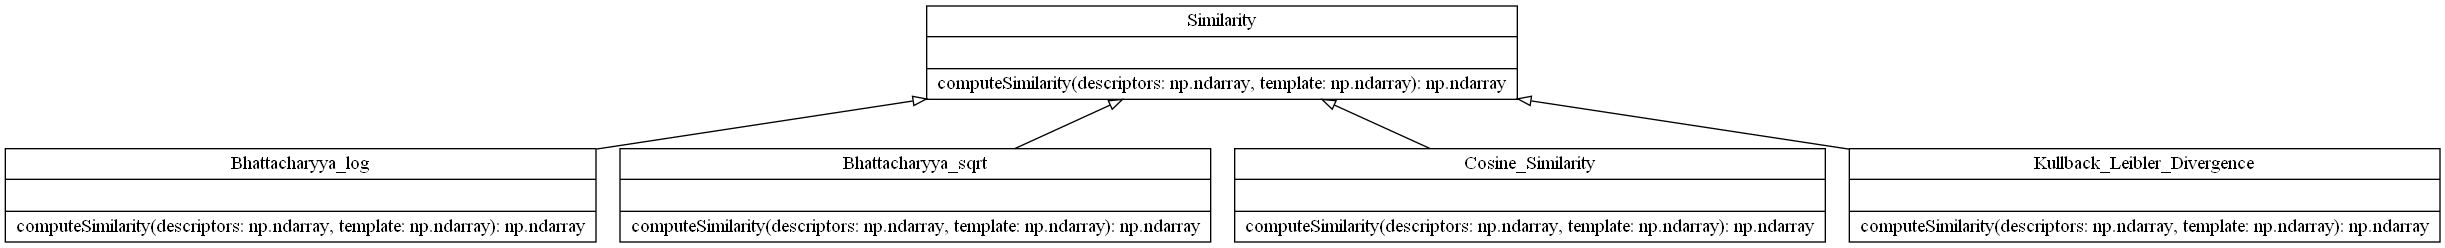
\includegraphics[scale=0.26,angle=90,origin=c]{similarity.png}}}
<<<<<<< HEAD
<<<<<<< HEAD
<<<<<<< HEAD
	\caption{Diagramme UML de la classe Similarity (\href{https://raw.githubusercontent.com/gabriel-combe/Cuttlefish_Tracker/main/rapport/UML/similarity.svg}{lien vers l'image SVG}, zoomer sur l'image SVG pour avoir plus de détaille).}
=======
	\caption{Diagramme UML de la classe Similarity (\href{https://raw.githubusercontent.com/gabriel-combe/Cuttlefish_Tracker/main/rapport/UML/similarity.svg}{lien vers l'image SVG}, zoomer sur l'image SVG pour avoir plus de détails).}
>>>>>>> a979539 (Fix typos)
=======
=======
>>>>>>> c164f46 (Rebase 6/7)
	\caption{Diagramme UML de la classe Similarity (\href{https://raw.githubusercontent.com/gabriel-combe/Cuttlefish_Tracker/main/rapport/UML/similarity.svg}{lien vers l'image SVG}, zoomer sur l'image SVG pour avoir plus de détails).}
=======
	\caption{Diagramme UML de la classe Similarity (\href{https://raw.githubusercontent.com/gabriel-combe/Cuttlefish_Tracker/test/rapport/UML/similarity.svg}{lien vers l'image SVG}, zoomer sur l'image SVG pour avoir plus de détaille).}
>>>>>>> afae3dc (Change diagram link for SVG)
<<<<<<< HEAD
>>>>>>> 0295ce9 (Rebase 4/7)
=======
=======
	\caption{Diagramme UML de la classe Similarity (\href{https://raw.githubusercontent.com/gabriel-combe/Cuttlefish_Tracker/main/rapport/UML/similarity.svg}{lien vers l'image SVG}, zoomer sur l'image SVG pour avoir plus de détaille).}
>>>>>>> f66402e (Fix typos)
>>>>>>> c164f46 (Rebase 6/7)
	\label{fig:uml_diagram_similarity}
\end{figure}
\FloatBarrier


\clearpage
\section*{Diagramme UML filtre à particule}\label{app:UMLParticleFilter}
\begin{figure}[!htbp]
	\center
		\subfloat{{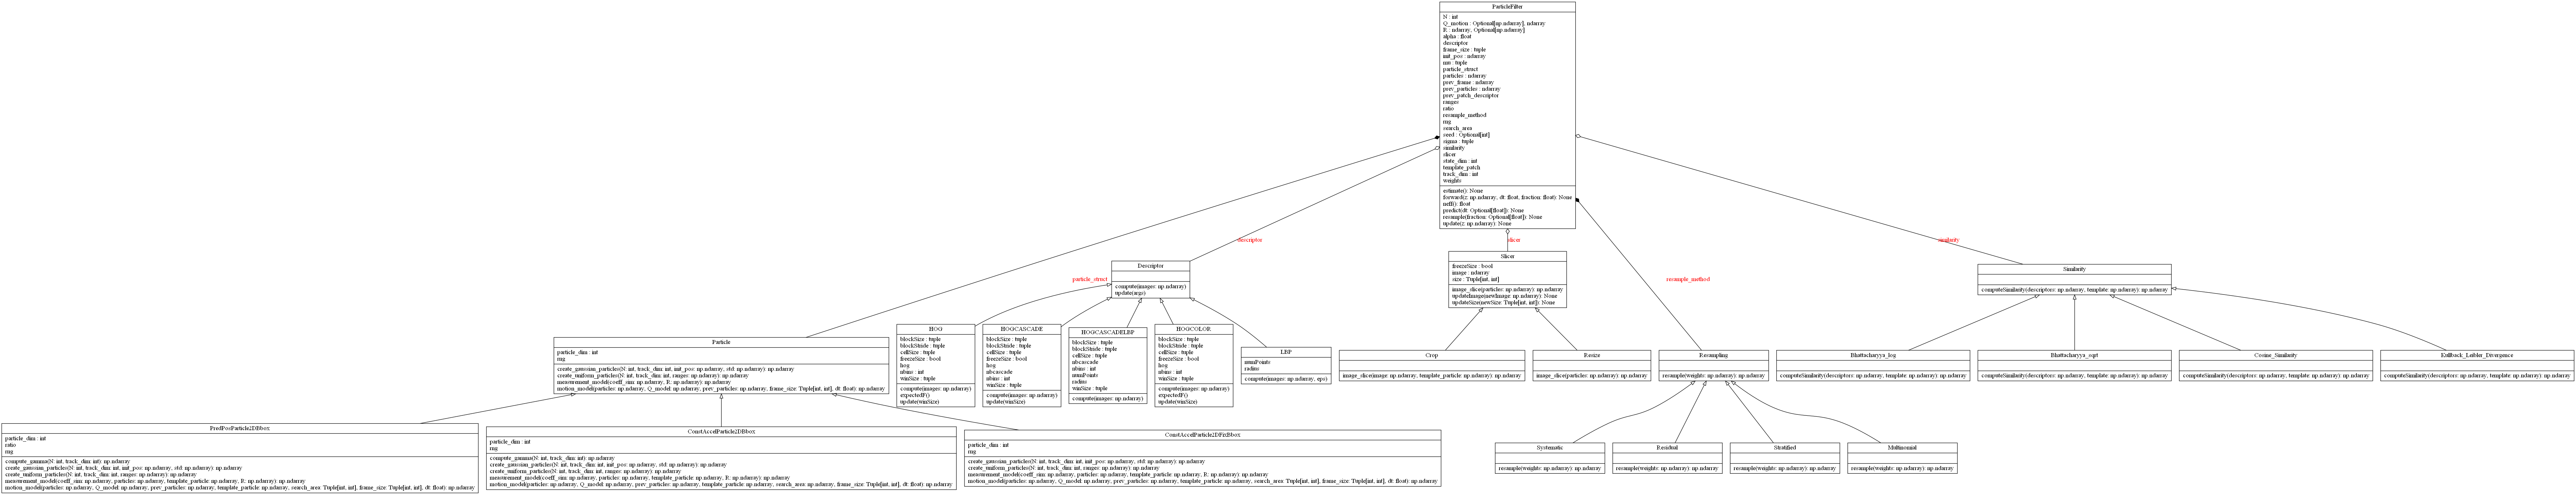
\includegraphics[scale=0.081,angle=90,origin=c]{particlefilter.png}}}
<<<<<<< HEAD
<<<<<<< HEAD
<<<<<<< HEAD
	\caption{Diagramme UML de la classe ParticleFilter (\href{https://raw.githubusercontent.com/gabriel-combe/Cuttlefish_Tracker/main/rapport/UML/particlefilter.svg}{lien vers l'image SVG}, zoomer sur l'image SVG pour avoir plus de détaille).}
=======
	\caption{Diagramme UML de la classe ParticleFilter (\href{https://raw.githubusercontent.com/gabriel-combe/Cuttlefish_Tracker/main/rapport/UML/particlefilter.svg}{lien vers l'image SVG}, zoomer sur l'image SVG pour avoir plus de détails).}
>>>>>>> a979539 (Fix typos)
=======
=======
>>>>>>> c164f46 (Rebase 6/7)
	\caption{Diagramme UML de la classe ParticleFilter (\href{https://raw.githubusercontent.com/gabriel-combe/Cuttlefish_Tracker/main/rapport/UML/particlefilter.svg}{lien vers l'image SVG}, zoomer sur l'image SVG pour avoir plus de détails).}
=======
	\caption{Diagramme UML de la classe ParticleFilter (\href{https://raw.githubusercontent.com/gabriel-combe/Cuttlefish_Tracker/test/rapport/UML/particlefilter.svg}{lien vers l'image SVG}, zoomer sur l'image SVG pour avoir plus de détaille).}
>>>>>>> afae3dc (Change diagram link for SVG)
<<<<<<< HEAD
>>>>>>> 0295ce9 (Rebase 4/7)
=======
=======
	\caption{Diagramme UML de la classe ParticleFilter (\href{https://raw.githubusercontent.com/gabriel-combe/Cuttlefish_Tracker/main/rapport/UML/particlefilter.svg}{lien vers l'image SVG}, zoomer sur l'image SVG pour avoir plus de détaille).}
>>>>>>> f66402e (Fix typos)
>>>>>>> c164f46 (Rebase 6/7)
	\label{fig:uml_diagram_particlefilter}
\end{figure}
\FloatBarrier
	
	
\clearpage
\section*{VAE (Variational Autoencoder)}\label{app:variational_autoencoder}
Les VAE, ou Variational Autoencoder, sont des réseaux de neurones qui essayent d'estimer une distribution probabiliste avec seulement un nombre limité d'échantillons provenant de cette distribution.\\
Ce genre de réseaux de neurones est divisé en deux parties:\\
\begin{itemize}
	\item \emph{Encodeur}\\
	Pour une donnée $x$, l'encodeur va projeter/compresser $x$ dans un espace de représentation plus petit (espace latent).\\
	L'encodeur a pour objectif de représenter $x$ de façon optimisée, et de conserver les informations les plus importantes.\\
	\item \emph{Décodeur}\\
	Pour une représentation issue de l'espace latent, le décodeur va essayer de décompresser/reconstruire $x$ en minimisant les pertes d'information.\\
	Le décodeur a pour objectif de produire une donnée $x'$ la plus similaire possible à $x$.\\
\end{itemize}
	
Le schéma global est illustré en figure \ref{fig:vae_scheme}.
\begin{figure}[!htbp]
\center
	\subfloat{{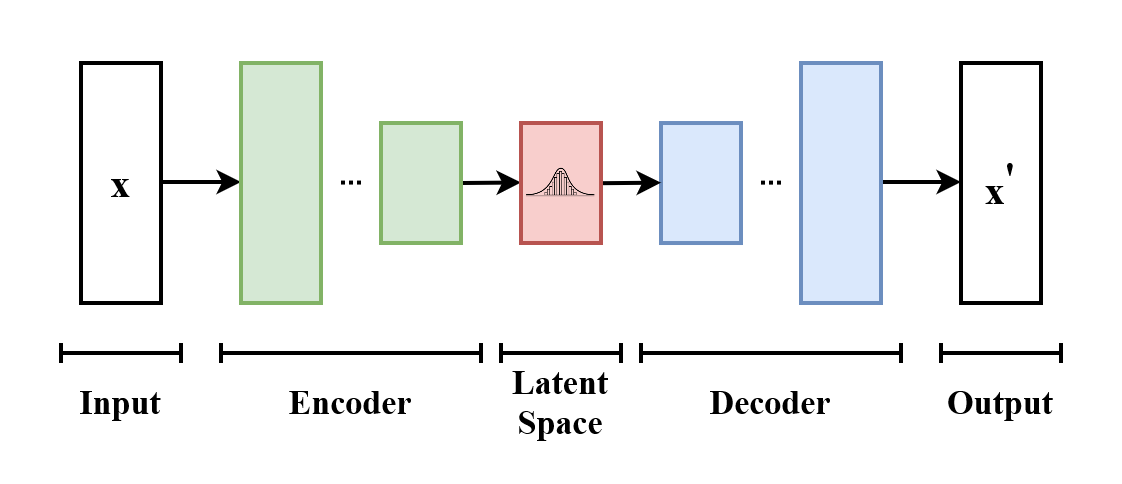
\includegraphics[scale=0.3]{VAE_Basic.png}}}
\caption{Schéma basique d'un VAE.}
\label{fig:vae_scheme}
\end{figure}
\FloatBarrier

\end{appendices}

\clearpage


\end{document}

